
%% bare_adv.tex
%% V1.4
%% 2012/12/27
%% by Michael Shell
%% See: 
%% http://www.michaelshell.org/
%% for current contact information.
%%
%% This is a skeleton file demonstrating the advanced use of IEEEtran.cls
%% (requires IEEEtran.cls version 1.8 or later) with an IEEE Computer
%% Society journal paper.
%%
%% Support sites:
%% http://www.michaelshell.org/tex/ieeetran/
%% http://www.ctan.org/tex-archive/macros/latex/contrib/IEEEtran/
%% and
%% http://www.ieee.org/

%%*************************************************************************
%% Legal Notice:
%% This code is offered as-is without any warranty either expressed or
%% implied; without even the implied warranty of MERCHANTABILITY or
%% FITNESS FOR A PARTICULAR PURPOSE! 
%% User assumes all risk.
%% In no event shall IEEE or any contributor to this code be liable for
%% any damages or losses, including, but not limited to, incidental,
%% consequential, or any other damages, resulting from the use or misuse
%% of any information contained here.
%%
%% All comments are the opinions of their respective authors and are not
%% necessarily endorsed by the IEEE.
%%
%% This work is distributed under the LaTeX Project Public License (LPPL)
%% ( http://www.latex-project.org/ ) version 1.3, and may be freely used,
%% distributed and modified. A copy of the LPPL, version 1.3, is included
%% in the base LaTeX documentation of all distributions of LaTeX released
%% 2003/12/01 or later.
%% Retain all contribution notices and credits.
%% ** Modified files should be clearly indicated as such, including  **
%% ** renaming them and changing author support contact information. **
%%
%% File list of work: IEEEtran.cls, IEEEtran_HOWTO.pdf, bare_adv.tex,
%%                    bare_conf.tex, bare_jrnl.tex, bare_jrnl_compsoc.tex,
%%                    bare_jrnl_transmag.tex
%%*************************************************************************

% *** Authors should verify (and, if needed, correct) their LaTeX system  ***
% *** with the testflow diagnostic prior to trusting their LaTeX platform ***
% *** with production work. IEEE's font choices can trigger bugs that do  ***
% *** not appear when using other class files.                            ***
% The testflow support page is at:
% http://www.michaelshell.org/tex/testflow/



% IEEEtran V1.7 and later provides for these CLASSINPUT macros to allow the
% user to reprogram some IEEEtran.cls defaults if needed. These settings
% override the internal defaults of IEEEtran.cls regardless of which class
% options are used. Do not use these unless you have good reason to do so as
% they can result in nonIEEE compliant documents. User beware. ;)
%
%\newcommand{\CLASSINPUTbaselinestretch}{1.0} % baselinestretch
%\newcommand{\CLASSINPUTinnersidemargin}{1in} % inner side margin
%\newcommand{\CLASSINPUToutersidemargin}{1in} % outer side margin
%\newcommand{\CLASSINPUTtoptextmargin}{1in}   % top text margin
%\newcommand{\CLASSINPUTbottomtextmargin}{1in}% bottom text margin



% Note that the a4paper option is mainly intended so that authors in
% countries using A4 can easily print to A4 and see how their papers will
% look in print - the typesetting of the document will not typically be
% affected with changes in paper size (but the bottom and side margins will).
% Use the testflow package mentioned above to verify correct handling of
% both paper sizes by the user's LaTeX system.
%
% Also note that the "draftcls" or "draftclsnofoot", not "draft", option
% should be used if it is desired that the figures are to be displayed in
% draft mode.
%
\documentclass[12pt,journal,compsoc]{IEEEtran}
% The Computer Society requires 12pt.
% If IEEEtran.cls has not been installed into the LaTeX system files,
% manually specify the path to it like:
% \documentclass[10pt,journal,compsoc]{../sty/IEEEtran}


% For Computer Society journals, IEEEtran defaults to the use of 
% Palatino/Palladio as is done in IEEE Computer Society journals.
% To go back to Times Roman, you can use this code:
%\renewcommand{\rmdefault}{ptm}\selectfont





% Some very useful LaTeX packages include:
% (uncomment the ones you want to load)



% *** MISC UTILITY PACKAGES ***
%
%\usepackage{ifpdf}
% Heiko Oberdiek's ifpdf.sty is very useful if you need conditional
% compilation based on whether the output is pdf or dvi.
% usage:
% \ifpdf
%   % pdf code
% \else
%   % dvi code
% \fi
% The latest version of ifpdf.sty can be obtained from:
% http://www.ctan.org/tex-archive/macros/latex/contrib/oberdiek/
% Also, note that IEEEtran.cls V1.7 and later provides a builtin
% \ifCLASSINFOpdf conditional that works the same way.
% When switching from latex to pdflatex and vice-versa, the compiler may
% have to be run twice to clear warning/error messages.






% *** CITATION PACKAGES ***
%
\ifCLASSOPTIONcompsoc
  % IEEE Computer Society needs nocompress option
  % requires cite.sty v4.0 or later (November 2003)
  % \usepackage[nocompress]{cite}
\else
  % normal IEEE
  % \usepackage{cite}
\fi
% cite.sty was written by Donald Arseneau
% V1.6 and later of IEEEtran pre-defines the format of the cite.sty package
% \cite{} output to follow that of IEEE. Loading the cite package will
% result in citation numbers being automatically sorted and properly
% "compressed/ranged". e.g., [1], [9], [2], [7], [5], [6] without using
% cite.sty will become [1], [2], [5]--[7], [9] using cite.sty. cite.sty's
% \cite will automatically add leading space, if needed. Use cite.sty's
% noadjust option (cite.sty V3.8 and later) if you want to turn this off
% such as if a citation ever needs to be enclosed in parenthesis.
% cite.sty is already installed on most LaTeX systems. Be sure and use
% version 4.0 (2003-05-27) and later if using hyperref.sty. cite.sty does
% not currently provide for hyperlinked citations.
% The latest version can be obtained at:
% http://www.ctan.org/tex-archive/macros/latex/contrib/cite/
% The documentation is contained in the cite.sty file itself.
%
% Note that some packages require special options to format as the Computer
% Society requires. In particular, Computer Society  papers do not use
% compressed citation ranges as is done in typical IEEE papers
% (e.g., [1]-[4]). Instead, they list every citation separately in order
% (e.g., [1], [2], [3], [4]). To get the latter we need to load the cite
% package with the nocompress option which is supported by cite.sty v4.0
% and later.
%
% Note also the use of a CLASSOPTION conditional provided by 
% IEEEtran.cls V1.7 and later.





% *** GRAPHICS RELATED PACKAGES ***
\usepackage{caption}
\ifCLASSINFOpdf
   \usepackage[pdftex]{graphicx}
  % declare the path(s) where your graphic files are
  % \graphicspath{{../pdf/}{../jpeg/}}
  % and their extensions so you won't have to specify these with
  % every instance of \includegraphics
  % \DeclareGraphicsExtensions{.pdf,.jpeg,.png}
\else
  % or other class option (dvipsone, dvipdf, if not using dvips). graphicx
  % will default to the driver specified in the system graphics.cfg if no
  % driver is specified.
  % \usepackage[dvips]{graphicx}
  % declare the path(s) where your graphic files are
  % \graphicspath{{../eps/}}
  % and their extensions so you won't have to specify these with
  % every instance of \includegraphics
  % \DeclareGraphicsExtensions{.eps}
\fi
% graphicx was written by David Carlisle and Sebastian Rahtz. It is
% required if you want graphics, photos, etc. graphicx.sty is already
% installed on most LaTeX systems. The latest version and documentation
% can be obtained at: 
% http://www.ctan.org/tex-archive/macros/latex/required/graphics/
% Another good source of documentation is "Using Imported Graphics in
% LaTeX2e" by Keith Reckdahl which can be found at:
% http://www.ctan.org/tex-archive/info/epslatex/
%
% latex, and pdflatex in dvi mode, support graphics in encapsulated
% postscript (.eps) format. pdflatex in pdf mode supports graphics
% in .pdf, .jpeg, .png and .mps (metapost) formats. Users should ensure
% that all non-photo figures use a vector format (.eps, .pdf, .mps) and
% not a bitmapped formats (.jpeg, .png). IEEE frowns on bitmapped formats
% which can result in "jaggedy"/blurry rendering of lines and letters as
% well as large increases in file sizes.
%
% You can find documentation about the pdfTeX application at:
% http://www.tug.org/applications/pdftex





% *** MATH PACKAGES ***
%
\usepackage[cmex10]{amsmath}
\usepackage{siunitx}
% A popular package from the American Mathematical Society that provides
% many useful and powerful commands for dealing with mathematics. If using
% it, be sure to load this package with the cmex10 option to ensure that
% only type 1 fonts will utilized at all point sizes. Without this option,
% it is possible that some math symbols, particularly those within
% footnotes, will be rendered in bitmap form which will result in a
% document that can not be IEEE Xplore compliant!
%
% Also, note that the amsmath package sets \interdisplaylinepenalty to 10000
% thus preventing page breaks from occurring within multiline equations. Use:
%\interdisplaylinepenalty=2500
% after loading amsmath to restore such page breaks as IEEEtran.cls normally
% does. amsmath.sty is already installed on most LaTeX systems. The latest
% version and documentation can be obtained at:
% http://www.ctan.org/tex-archive/macros/latex/required/amslatex/math/





% *** SPECIALIZED LIST PACKAGES ***
%\usepackage{acronym}
% acronym.sty was written by Tobias Oetiker. This package provides tools for
% managing documents with large numbers of acronyms. (You don't *have* to
% use this package - unless you have a lot of acronyms, you may feel that
% such package management of them is bit of an overkill.)
% Do note that the acronym environment (which lists acronyms) will have a
% problem when used under IEEEtran.cls because acronym.sty relies on the
% description list environment - which IEEEtran.cls has customized for
% producing IEEE style lists. A workaround is to declared the longest
% label width via the IEEEtran.cls \IEEEiedlistdecl global control:
%
% \renewcommand{\IEEEiedlistdecl}{\IEEEsetlabelwidth{SONET}}
% \begin{acronym}
%
% \end{acronym}
% \renewcommand{\IEEEiedlistdecl}{\relax}% remember to reset \IEEEiedlistdecl
%
% instead of using the acronym environment's optional argument.
% The latest version and documentation can be obtained at:
% http://www.ctan.org/tex-archive/macros/latex/contrib/acronym/


%\usepackage{algorithmic}
% algorithmic.sty was written by Peter Williams and Rogerio Brito.
% This package provides an algorithmic environment fo describing algorithms.
% You can use the algorithmic environment in-text or within a figure
% environment to provide for a floating algorithm. Do NOT use the algorithm
% floating environment provided by algorithm.sty (by the same authors) or
% algorithm2e.sty (by Christophe Fiorio) as IEEE does not use dedicated
% algorithm float types and packages that provide these will not provide
% correct IEEE style captions. The latest version and documentation of
% algorithmic.sty can be obtained at:
% http://www.ctan.org/tex-archive/macros/latex/contrib/algorithms/
% There is also a support site at:
% http://algorithms.berlios.de/index.html
% Also of interest may be the (relatively newer and more customizable)
% algorithmicx.sty package by Szasz Janos:
% http://www.ctan.org/tex-archive/macros/latex/contrib/algorithmicx/




% *** ALIGNMENT PACKAGES ***
%
\usepackage{array}
% Frank Mittelbach's and David Carlisle's array.sty patches and improves
% the standard LaTeX2e array and tabular environments to provide better
% appearance and additional user controls. As the default LaTeX2e table
% generation code is lacking to the point of almost being broken with
% respect to the quality of the end results, all users are strongly
% advised to use an enhanced (at the very least that provided by array.sty)
% set of table tools. array.sty is already installed on most systems. The
% latest version and documentation can be obtained at:
% http://www.ctan.org/tex-archive/macros/latex/required/tools/


%\usepackage{mdwmath}
%\usepackage{mdwtab}
% Also highly recommended is Mark Wooding's extremely powerful MDW tools,
% especially mdwmath.sty and mdwtab.sty which are used to format equations
% and tables, respectively. The MDWtools set is already installed on most
% LaTeX systems. The lastest version and documentation is available at:
% http://www.ctan.org/tex-archive/macros/latex/contrib/mdwtools/


% IEEEtran contains the IEEEeqnarray family of commands that can be used to
% generate multiline equations as well as matrices, tables, etc., of high
% quality.


%\usepackage{eqparbox}
% Also of notable interest is Scott Pakin's eqparbox package for creating
% (automatically sized) equal width boxes - aka "natural width parboxes".
% Available at:
% http://www.ctan.org/tex-archive/macros/latex/contrib/eqparbox/




% *** SUBFIGURE PACKAGES ***
%\ifCLASSOPTIONcompsoc
%  \usepackage[caption=false,font=normalsize,labelfont=sf,textfont=sf]{subfig}
%\else
%  \usepackage[caption=false,font=footnotesize]{subfig}
%\fi
% subfig.sty, written by Steven Douglas Cochran, is the modern replacement
% for subfigure.sty, the latter of which is no longer maintained and is
% incompatible with some LaTeX packages including fixltx2e. However,
% subfig.sty requires and automatically loads Axel Sommerfeldt's caption.sty
% which will override IEEEtran.cls' handling of captions and this will result
% in non-IEEE style figure/table captions. To prevent this problem, be sure
% and invoke subfig.sty's "caption=false" package option (available since
% subfig.sty version 1.3, 2005/06/28) as this is will preserve IEEEtran.cls
% handling of captions.
% Note that the Computer Society format requires a larger sans serif font
% than the serif footnote size font used in traditional IEEE formatting
% and thus the need to invoke different subfig.sty package options depending
% on whether compsoc mode has been enabled.
%
% The latest version and documentation of subfig.sty can be obtained at:
% http://www.ctan.org/tex-archive/macros/latex/contrib/subfig/




% *** FLOAT PACKAGES ***
%
%\usepackage{fixltx2e}
% fixltx2e, the successor to the earlier fix2col.sty, was written by
% Frank Mittelbach and David Carlisle. This package corrects a few problems
% in the LaTeX2e kernel, the most notable of which is that in current
% LaTeX2e releases, the ordering of single and double column floats is not
% guaranteed to be preserved. Thus, an unpatched LaTeX2e can allow a
% single column figure to be placed prior to an earlier double column
% figure. The latest version and documentation can be found at:
% http://www.ctan.org/tex-archive/macros/latex/base/

\usepackage[section]{placeins}
\usepackage{stfloats}
% stfloats.sty was written by Sigitas Tolusis. This package gives LaTeX2e
% the ability to do double column floats at the bottom of the page as well
% as the top. (e.g., "\begin{figure*}[!b]" is not normally possible in
% LaTeX2e). It also provides a command:
%\fnbelowfloat
% to enable the placement of footnotes below bottom floats (the standard
% LaTeX2e kernel puts them above bottom floats). This is an invasive package
% which rewrites many portions of the LaTeX2e float routines. It may not work
% with other packages that modify the LaTeX2e float routines. The latest
% version and documentation can be obtained at:
% http://www.ctan.org/tex-archive/macros/latex/contrib/sttools/
% Do not use the stfloats baselinefloat ability as IEEE does not allow
% \baselineskip to stretch. Authors submitting work to the IEEE should note
% that IEEE rarely uses double column equations and that authors should try
% to avoid such use. Do not be tempted to use the cuted.sty or midfloat.sty
% packages (also by Sigitas Tolusis) as IEEE does not format its papers in
% such ways.
% Do not attempt to use stfloats with fixltx2e as they are incompatible.
% Instead, use Morten Hogholm'a dblfloatfix which combines the features
% of both fixltx2e and stfloats:
%
% \usepackage{dblfloatfix}
% The latest version can be found at:
% http://www.ctan.org/tex-archive/macros/latex/contrib/dblfloatfix/


%\ifCLASSOPTIONcaptionsoff
%  \usepackage[nomarkers]{endfloat}
% \let\MYoriglatexcaption\caption
% \renewcommand{\caption}[2][\relax]{\MYoriglatexcaption[#2]{#2}}
%\fi
% endfloat.sty was written by James Darrell McCauley, Jeff Goldberg and 
% Axel Sommerfeldt. This package may be useful when used in conjunction with 
% IEEEtran.cls'  captionsoff option. Some IEEE journals/societies require that
% submissions have lists of figures/tables at the end of the paper and that
% figures/tables without any captions are placed on a page by themselves at
% the end of the document. If needed, the draftcls IEEEtran class option or
% \CLASSINPUTbaselinestretch interface can be used to increase the line
% spacing as well. Be sure and use the nomarkers option of endfloat to
% prevent endfloat from "marking" where the figures would have been placed
% in the text. The two hack lines of code above are a slight modification of
% that suggested by in the endfloat docs (section 8.4.1) to ensure that
% the full captions always appear in the list of figures/tables - even if
% the user used the short optional argument of \caption[]{}.
% IEEE papers do not typically make use of \caption[]'s optional argument,
% so this should not be an issue. A similar trick can be used to disable
% captions of packages such as subfig.sty that lack options to turn off
% the subcaptions:
% For subfig.sty:
% \let\MYorigsubfloat\subfloat
% \renewcommand{\subfloat}[2][\relax]{\MYorigsubfloat[]{#2}}
% However, the above trick will not work if both optional arguments of
% the \subfloat command are used. Furthermore, there needs to be a
% description of each subfigure *somewhere* and endfloat does not add
% subfigure captions to its list of figures. Thus, the best approach is to
% avoid the use of subfigure captions (many IEEE journals avoid them anyway)
% and instead reference/explain all the subfigures within the main caption.
% The latest version of endfloat.sty and its documentation can obtained at:
% http://www.ctan.org/tex-archive/macros/latex/contrib/endfloat/
%
% The IEEEtran \ifCLASSOPTIONcaptionsoff conditional can also be used
% later in the document, say, to conditionally put the References on a 
% page by themselves.





% *** PDF, URL AND HYPERLINK PACKAGES ***
%
%\usepackage{url}
% url.sty was written by Donald Arseneau. It provides better support for
% handling and breaking URLs. url.sty is already installed on most LaTeX
% systems. The latest version and documentation can be obtained at:
% http://www.ctan.org/tex-archive/macros/latex/contrib/url/
% Basically, \url{my_url_here}.


% NOTE: PDF thumbnail features are not required in IEEE papers
%       and their use requires extra complexity and work.
%\ifCLASSINFOpdf
%  \usepackage[pdftex]{thumbpdf}
%\else
%  \usepackage[dvips]{thumbpdf}
%\fi
% thumbpdf.sty and its companion Perl utility were written by Heiko Oberdiek.
% It allows the user a way to produce PDF documents that contain fancy
% thumbnail images of each of the pages (which tools like acrobat reader can
% utilize). This is possible even when using dvi->ps->pdf workflow if the
% correct thumbpdf driver options are used. thumbpdf.sty incorporates the
% file containing the PDF thumbnail information (filename.tpm is used with
% dvips, filename.tpt is used with pdftex, where filename is the base name of
% your tex document) into the final ps or pdf output document. An external
% utility, the thumbpdf *Perl script* is needed to make these .tpm or .tpt
% thumbnail files from a .ps or .pdf version of the document (which obviously
% does not yet contain pdf thumbnails). Thus, one does a:
% 
% thumbpdf filename.pdf 
%
% to make a filename.tpt, and:
%
% thumbpdf --mode dvips filename.ps
%
% to make a filename.tpm which will then be loaded into the document by
% thumbpdf.sty the NEXT time the document is compiled (by pdflatex or
% latex->dvips->ps2pdf). Users must be careful to regenerate the .tpt and/or
% .tpm files if the main document changes and then to recompile the
% document to incorporate the revised thumbnails to ensure that thumbnails
% match the actual pages. It is easy to forget to do this!
% 
% Unix systems come with a Perl interpreter. However, MS Windows users
% will usually have to install a Perl interpreter so that the thumbpdf
% script can be run. The Ghostscript PS/PDF interpreter is also required.
% See the thumbpdf docs for details. The latest version and documentation
% can be obtained at.
% http://www.ctan.org/tex-archive/support/thumbpdf/


% NOTE: PDF hyperlink and bookmark features are not required in IEEE
%       papers and their use requires extra complexity and work.
% *** IF USING HYPERREF BE SURE AND CHANGE THE EXAMPLE PDF ***
% *** TITLE/SUBJECT/AUTHOR/KEYWORDS INFO BELOW!!           ***
\newcommand\MYhyperrefoptions{bookmarks=true,bookmarksnumbered=true,
pdfpagemode={UseOutlines},plainpages=false,pdfpagelabels=true,
colorlinks=true,linkcolor={black},citecolor={black},urlcolor={black},
pdftitle={Bare Demo of IEEEtran.cls for Computer Society Journals},%<!CHANGE!
pdfsubject={Typesetting},%<!CHANGE!
pdfauthor={Michael D. Shell},%<!CHANGE!
pdfkeywords={Computer Society, IEEEtran, journal, LaTeX, paper,
             template}}%<^!CHANGE!
%\ifCLASSINFOpdf
%\usepackage[\MYhyperrefoptions,pdftex]{hyperref}
%\else
%\usepackage[\MYhyperrefoptions,breaklinks=true,dvips]{hyperref}
%\usepackage{breakurl}
%\fi
% One significant drawback of using hyperref under DVI output is that the
% LaTeX compiler cannot break URLs across lines or pages as can be done
% under pdfLaTeX's PDF output via the hyperref pdftex driver. This is
% probably the single most important capability distinction between the
% DVI and PDF output. Perhaps surprisingly, all the other PDF features
% (PDF bookmarks, thumbnails, etc.) can be preserved in
% .tex->.dvi->.ps->.pdf workflow if the respective packages/scripts are
% loaded/invoked with the correct driver options (dvips, etc.). 
% As most IEEE papers use URLs sparingly (mainly in the references), this
% may not be as big an issue as with other publications.
%
% That said, Vilar Camara Neto created his breakurl.sty package which
% permits hyperref to easily break URLs even in dvi mode.
% Note that breakurl, unlike most other packages, must be loaded
% AFTER hyperref. The latest version of breakurl and its documentation can
% be obtained at:
% http://www.ctan.org/tex-archive/macros/latex/contrib/breakurl/
% breakurl.sty is not for use under pdflatex pdf mode.
%
% The advanced features offer by hyperref.sty are not required for IEEE
% submission, so users should weigh these features against the added
% complexity of use.
% The package options above demonstrate how to enable PDF bookmarks
% (a type of table of contents viewable in Acrobat Reader) as well as
% PDF document information (title, subject, author and keywords) that is
% viewable in Acrobat reader's Document_Properties menu. PDF document
% information is also used extensively to automate the cataloging of PDF
% documents. The above set of options ensures that hyperlinks will not be
% colored in the text and thus will not be visible in the printed page,
% but will be active on "mouse over". USING COLORS OR OTHER HIGHLIGHTING
% OF HYPERLINKS CAN RESULT IN DOCUMENT REJECTION BY THE IEEE, especially if
% these appear on the "printed" page. IF IN DOUBT, ASK THE RELEVANT
% SUBMISSION EDITOR. You may need to add the option hypertexnames=false if
% you used duplicate equation numbers, etc., but this should not be needed
% in normal IEEE work.
% The latest version of hyperref and its documentation can be obtained at:
% http://www.ctan.org/tex-archive/macros/latex/contrib/hyperref/





% *** Do not adjust lengths that control margins, column widths, etc. ***
% *** Do not use packages that alter fonts (such as pslatex).         ***
% There should be no need to do such things with IEEEtran.cls V1.6 and later.
% (Unless specifically asked to do so by the journal or conference you plan
% to submit to, of course. )


% correct bad hyphenation here
\hyphenation{op-tical net-works semi-conduc-tor}


\begin{document}
%
% paper title
% can use linebreaks \\ within to get better formatting as desired
% Do not put math or special symbols in the title.
\title{Two Wheel Drive Electronic Differential\\ \large{NC State Engineering at UNC Asheville\\Senior Design 2014}}
%
%
% author names and IEEE memberships
% note positions of commas and nonbreaking spaces ( ~ ) LaTeX will not break
% a structure at a ~ so this keeps an author's name from being broken across
% two lines.
% use \thanks{} to gain access to the first footnote area
% a separate \thanks must be used for each paragraph as LaTeX2e's \thanks
% was not built to handle multiple paragraphs
%
%
%\IEEEcompsocitemizethanks is a special \thanks that produces the bulleted
% lists the Computer Society journals use for "first footnote" author
% affiliations. Use \IEEEcompsocthanksitem which works much like \item
% for each affiliation group. When not in compsoc mode,
% \IEEEcompsocitemizethanks becomes like \thanks and
% \IEEEcompsocthanksitem becomes a line break with idention. This
% facilitates dual compilation, although admittedly the differences in the
% desired content of \author between the different types of papers makes a
% one-size-fits-all approach a daunting prospect. For instance, compsoc 
% journal papers have the author affiliations above the "Manuscript
% received ..."  text while in non-compsoc journals this is reversed. Sigh.

\author{

\centering
\begin{tabular}{c c c} 
\small{Jennifer~Cory}    &    \small{ Nathan~Lewis}        &  \small{Jason~Shores}        \\
\small{Nick~Faught }        &  \small{  Jason~McCrary}     &  \small{ Bryan~Short  }          \\ 
\small{Robert~Fussell}    &   \small{ Cullen~Reed   }      &   \small{Rachael~Stanfield}  \\
\small{Jason~Hopper  }   &   \small{Hallie~Sheaffer }    &  \small{ Gus~Tabaileh   }       \\
\small{Dakota~Lazenby} &                                                  &  \small{ Brandon~Zschokke} \\
\end{tabular} 



%\IEEEcompsocitemizethanks{\IEEEcompsocthanksitem M. Shell is with the Department
%of Electrical and Computer Engineering, Georgia Institute of Technology, Atlanta,
%GA, 30332.\protect\\
%% note need leading \protect in front of \\ to get a newline within \thanks as
%% \\ is fragile and will error, could use \hfil\break instead.
%E-mail: see http://www.michaelshell.org/contact.html
%\IEEEcompsocthanksitem J. Doe and J. Doe are with Anonymous University.}% <-this % stops a space
\thanks{EGM 485-602 Two Wheel Drive Electronic Differential}

}

% note the % following the last \IEEEmembership and also \thanks - 
% these prevent an unwanted space from occurring between the last author name
% and the end of the author line. i.e., if you had this:
% 
% \author{....lastname \thanks{...} \thanks{...} }
%                     ^------------^------------^----Do not want these spaces!
%
% a space would be appended to the last name and could cause every name on that
% line to be shifted left slightly. This is one of those "LaTeX things". For
% instance, "\textbf{A} \textbf{B}" will typeset as "A B" not "AB". To get
% "AB" then you have to do: "\textbf{A}\textbf{B}"
% \thanks is no different in this regard, so shield the last } of each \thanks
% that ends a line with a % and do not let a space in before the next \thanks.
% Spaces after \IEEEmembership other than the last one are OK (and needed) as
% you are supposed to have spaces between the names. For what it is worth,
% this is a minor point as most people would not even notice if the said evil
% space somehow managed to creep in.



% The paper headers
\markboth{University of North Carolina at Asheville Undergraduate Research}%
{Shell \MakeLowercase{\textit{et al.}}: Bare Advanced Demo of IEEEtran.cls for Journals}
% The only time the second header will appear is for the odd numbered pages
% after the title page when using the twoside option.
% 
% *** Note that you probably will NOT want to include the author's ***
% *** name in the headers of peer review papers.                   ***
% You can use \ifCLASSOPTIONpeerreview for conditional compilation here if
% you desire.



% The publisher's ID mark at the bottom of the page is less important with
% Computer Society journal papers as those publications place the marks
% outside of the main text columns and, therefore, unlike regular IEEE
% journals, the available text space is not reduced by their presence.
% If you want to put a publisher's ID mark on the page you can do it like
% this:
%\IEEEpubid{0000--0000/00\$00.00~\copyright~2012 IEEE}
% or like this to get the Computer Society new two part style.
%\IEEEpubid{\makebox[\columnwidth]{\hfill 0000--0000/00/\$00.00~\copyright~2012 IEEE}%
%\hspace{\columnsep}\makebox[\columnwidth]{Published by the IEEE Computer Society\hfill}}
% Remember, if you use this you must call \IEEEpubidadjcol in the second
% column for its text to clear the IEEEpubid mark (Computer Society journal
% papers don't need this extra clearance.)



% use for special paper notices
%\IEEEspecialpapernotice{(Invited Paper)}



% for Computer Society papers, we must declare the abstract and index terms
% PRIOR to the title within the \IEEEtitleabstractindextext IEEEtran
% command as these need to go into the title area created by \maketitle.
% As a general rule, do not put math, special symbols or citations
% in the abstract or keywords.
\IEEEtitleabstractindextext{
\begin{abstract}
The 2013-14 UNC Asheville / NC State Mechatronics Senior Project team designed and built an electronically controlled, differentially driven, two wheel drive vehicle.  The vehicle employs a student-designed and constructed drive system; integrating two electric motors, two controllers, and necessary sensors under the supervisory control of a microprocessor.
The vehicle hardware allows for comparison of two rear axle configurations:  1) a single, solid axle, with both wheels rotating in unison; and 2) a pair of independent axles, each with its own motor, controlled to provide differential operation.  Appropriate control schemes were implemented via a feedback loop through the microprocessor.  Standard automotive industry tests were adapted to gauge the change in performance between the modes.
One primary motivation for the project is to provide a ``proof of concept'' demonstrator.  With further refinement beyond the work presented here, future student teams will be able to use the vehicle to showcase the UNC Asheville / NC State Mechatronics Program's capabilities to potential academic collaborators.


\end{abstract}

% Note that keywords are not normally used for peerreview papers.
%\begin{IEEEkeywords}
%Computer Society, IEEEtran, journal, \LaTeX, paper, template.
%\end{IEEEkeywords}
}


% make the title area
\maketitle


% To allow for easy dual compilation without having to reenter the
% abstract/keywords data, the \IEEEtitleabstractindextext text will
% not be used in maketitle, but will appear (i.e., to be "transported")
% here as \IEEEdisplaynontitleabstractindextext when compsoc mode
% is not selected <OR> if conference mode is selected - because compsoc
% conference papers position the abstract like regular (non-compsoc)
% papers do!
\IEEEdisplaynontitleabstractindextext
% \IEEEdisplaynontitleabstractindextext has no effect when using
% compsoc under a non-conference mode.


% For peer review papers, you can put extra information on the cover
% page as needed:
% \ifCLASSOPTIONpeerreview
% \begin{center} \bfseries EDICS Category: 3-BBND \end{center}
% \fi
%
% For peerreview papers, this IEEEtran command inserts a page break and
% creates the second title. It will be ignored for other modes.
\IEEEpeerreviewmaketitle



%////////////////////////////////////////////////////////////////////////////////////////////////////////////////////////////////////////////////////////////////////////////////////////////////////////////////////////////////////////
% INTRODUCTION
%////////////////////////////////////////////////////////////////////////////////////////////////////////////////////////////////////////////////////////////////////////////////////////////////////////////////////////////////////////


% Computer Society journal papers do something a tad strange with the very
% first section heading (almost always called "Introduction"). They place it
% ABOVE the main text! IEEEtran.cls currently does not do this for you.
% However, You can achieve this effect by making LaTeX jump through some
% hoops via something like:
%
%\ifCLASSOPTIONcompsoc
%  \noindent\raisebox{2\baselineskip}[0pt][0pt]%
%  {\parbox{\columnwidth}{\section{Introduction}\label{sec:introduction}%
%  \global\everypar=\everypar}}%
%  \vspace{-1\baselineskip}\vspace{-\parskip}\par
%\else
%  \section{Introduction}\label{sec:introduction}\par
%\fi
%
% Admittedly, this is a hack and may well be fragile, but seems to do the
% trick for me. Note the need to keep any \label that may be used right
% after \section in the above as the hack puts \section within a raised box.



% The very first letter is a 2 line initial drop letter followed
% by the rest of the first word in caps (small caps for compsoc).
% 
% form to use if the first word consists of a single letter:
% \IEEEPARstart{A}{demo} file is ....
% 
% form to use if you need the single drop letter followed by
% normal text (unknown if ever used by IEEE):
% \IEEEPARstart{A}{}demo file is ....
% 
% Some journals put the first two words in caps:
% \IEEEPARstart{T}{his demo} file is ....
% 
% Here we have the typical use of a "T" for an initial drop letter
% and "HIS" in caps to complete the first word.

% You must have at least 2 lines in the paragraph with the drop letter
% (should never be an issue)
\section{Introduction}
\subsection{Institutional Background}
\IEEEPARstart{T}{he} Mechatronics Engineering program at UNC Asheville is a hybrid of the electrical, mechanical and computer engineering disciplines. EGM 484 and 485, the classes which constitute the senior design project, are designed to allow the students creative license on a project that uses all of the skills learned in the first three years of the program. The project also introduces project management techniques such as budgeting, goal setting and task management. 
	
	Formula SAE (FSAE), sanctioned by the Society of Automotive Engineers, offers a highly attractive venue for learning, applying, and demonstrating automotive engineering skills in a relevant, fun, hands-on competition. Unfortunately, successful FSAE efforts demand a level of resources beyond the present capabilities and budget of the NC State / UNC Asheville Mechatronics program; however, because Mechatronics specializes in the computer control of electromechanical systems, it is reasonable to think that UNC Asheville could serve as an electric drivetrain ``subcontractor'' to an existing FSAE team on another campus. Such a joint venture would provide a staged entry into FSAE for UNC Asheville, with the possibility of building toward a completely in-house effort over time. 
	
	The goal of this year's senior project is to design and build a vehicle employing an electronic differential.  The underlying goal of the project, in demonstrating an improvement in performance via this differential control, is the pursuit of increasing the likelihood of a larger team adopting the UNC Asheville/NCSU program as a subcontractor for its expertise in control of integrated electronic and mechanical systems.  Since the drive system's control is the most technologically challenging aspect of the project, the successful implementation of a low power, two-wheel drive system on a simple vehicle should serve as an adequate advertisement for the Mechatronics Program's capabilities.  As a result, success in this collaboration allows for a more competitive electric vehicle in teams that have previously been traditionally divided between strictly mechanical and electrical engineers. This initial step taken by the current senior design group also allows future undergraduate students to continue improving upon the existing control systems, as well formulating and developing partnerships with other universities. In addition, setting this framework increases general awareness of the Mechatronics program at UNC Asheville in attempts to create potential to attract new students.   

\subsection{Technical Background}
	
	In addition to increased energy efficiency and a reduction in harmful emissions, powering a vehicle electrically offers opportunities for significant improvements in stability and handling.  This increased stability and traction is particularly useful in conditions where traction is inconsistent or compromised by conditions such as rain, snow, and off-road situations.  Differential control of the driven wheels facilitates an improvement in cornering precision and reduces the net power demand from the drivetrain.  Independently driven wheels also have a place in motorsports, allowing for increases in cornering speeds and increased handling.  This increase in performance is due to better controlling the vehicle dynamics.  When cornering, the wheel on the outside of the turn rotates faster than the one on the inside. Most mechanical differentials compensate for this through a system of gears that allows one wheel to spin slower than the other when the vehicle is in a turn.  In a mechanical differential, the average of the angular speeds of the the drive wheels is equal to the rotational speed of the input shaft to the differential.  The senior design team's experimental system mimics these mechanical systems on our split axle, electric system.  
	
	The design of the electronic differential keeps both wheels under power and is tuned to differ the throttle to each motor to allow variable wheel speeds while still providing the requested vehicle velocity around a turn. The difference in speeds depends upon the turning angle, measured from the steering shaft, and the throttle input.  These user inputs are then used in calculations inside the microcontroller to decide the theoretical difference in wheel speeds and then to vary the throttle out of the controller accordingly.  This is the functionality of the open loop control scheme.  The closed loop control then takes the wheel speed, referenced from the encoders attached to the motors, and verifies the effect of differing the throttle to the two motors.  If the difference is not enough, then our control law then increases the difference in throttle to increase the difference in wheel speed.  Equivalently, should the wheel speeds be too far apart, then the control law reduces the difference in throttle applied to the motors to bring the wheel speeds closer together.        

%\hfill mds
% 
%\hfill December 27, 2012

%\subsection{Subsection Heading Here}
%Subsection text here.
%
%% needed in second column of first page if using \IEEEpubid
%%\IEEEpubidadjcol
%
%\subsubsection{Subsubsection Heading Here}
%Subsubsection text here.

%////////////////////////////////////////////////////////////////////////////////////////////////////////////////////////////////////////////////////////////////////////////////////////////////////////////////////////////////////////
% OVERVIEW
%////////////////////////////////////////////////////////////////////////////////////////////////////////////////////////////////////////////////////////////////////////////////////////////////////////////////////////////////////////
\section{Project Overview}

	The project team chose the electronic differential project and defined its success as the demonstration of improved performance when utilizing the differentially controlled rear wheels in comparison with the solid axle.  In pursuit of this success, the team had to decide what parts to acquire and how to assemble the parts into a coherent and effective design that would demonstrate the performance increase sought after.  
	
	The initial decision made was that the vehicle must be capable of at least two modes of operation:

	1) The first mode must allow the separate drive axles to be coupled mechanically into a single solid axle. The control system would then allow the motors to exert the same total force available in the second mode by applying equal amounts of throttle, and thus equal amounts of drive force to the live axle. 

	2) The second mode must involve two independently driven axles, each with its own motor. This type of control would then allow the two sides to turn independently at speeds determined by the control system. The control system must include the necessary components and code to discern the driver's intentions and provide the correct response.

	The team, after having made the specifications listed above, then commenced to do research as to what motors and controllers could be acquired, what chassis to install the system on, and what sensors and controller to employ in creating the completed system.  The major factor that guided decisions concerning parts acquisition was budgetary restrictions.  After having obtained most key parts from donations, the team then purchased, from the budgeted fund, parts to complement the donations.  
	
	After acquiring most of the parts, construction ensued.  This construction many problems.  Fighting the bent chassis, installing a full electric system on a chassis meant for a small gasoline motor, and many other problems presented themselves as the team furiously attempted to construct the system.  Construction, as a result of these problems, took far longer than expected and left little time for controller design and fine tuning.  Nearing the end of the project deadlines, the team found that there was just insufficient time to devise a complicated and well oiled controller and thus resolved to implement a rudimentary controller and then provide sufficient notes to allow for improvement by later teams.

%////////////////////////////////////////////////////////////////////////////////////////////////////////////////////////////////////////////////////////////////////////////////////////////////////////////////////////////////////////
% PRELIMINARY DESIGN
%////////////////////////////////////////////////////////////////////////////////////////////////////////////////////////////////////////////////////////////////////////////////////////////////////////////////////////////////////////


\section{Preliminary Design}
\subsection{Objectives}
The primary objectives of the team were as follows:
	
	1) Acquire parts to construct a fully electric vehicle and implement a control system on the vehicle all within budgetary limitations of two-thousand dollars of expenditure.
	
	2) Construct the electric vehicle to hold at least one person (driver).

	3) Construct a drivetrain that allows for two independent motors driving two independent axles and wheels, while allowing the axles to be coupled for ``live axle'' driving.

	4) Implement a control system to provide variant throttle to the motors, thus controlling the wheels speeds in a differential manner.

	5) Retain a sufficient level of safety for the driver to prevent severe bodily harm in the event of system mayhem, and potential loss of user control.

\subsection{Team Management}

	The project team was initially split into three main divisions with groups of team members assigned to sub-teams.  Each team reported to a designated overseer.  The three sections were:

	1) Fabrication/Mechanical: The team working on this section was responsible for carrying out all of the mechanical operations necessary to create a working vehicle.  The donated chassis required significant mechanical modification to satisfy the project requirements.  These modifications mainly consisted of converting the vehicle from a single axle gas powered setup to an electronic two axle system.

	2) Electrical:  The vehicle drive system consists of several electrical components, including sensors,  a microcontroller, motors, and programmable motor controllers.  It was the responsibility of the electrical team to research, procure, and implement these items.

	3) Programming/Controls:  The team working on this section was responsible for implementing the algorithms necessary to achieve differential control.  This requires programming code to take sensor input and produce a controlled output.
	
	In addition to their specific responsibilities, each team was also responsible for documenting the processes used to achieve their goals.  Operating in this manner assured that future teams could refer to the notes set forth by this team in attempts to continue and progress with this project, or to use parts of it to aid with other future projects.  By the end of this project, the teams dissolved and formed a smaller group.  The smaller group consisted of the most knowledgeable members of the prior group, these leaders then collaborated as one ``interdisciplinary'' team. 

\subsection{Models}
\subsubsection{Chassis}
One of the first models created was a \emph{SolidWorks} model of the donated chassis. The 3D model allowed the team to visually inspect and determine proper locations of various components before permanently mounting them to the chassis. The chassis model can be seen in Figure~\ref{solidworks_model}.

\begin{figure}[!h]
\centering
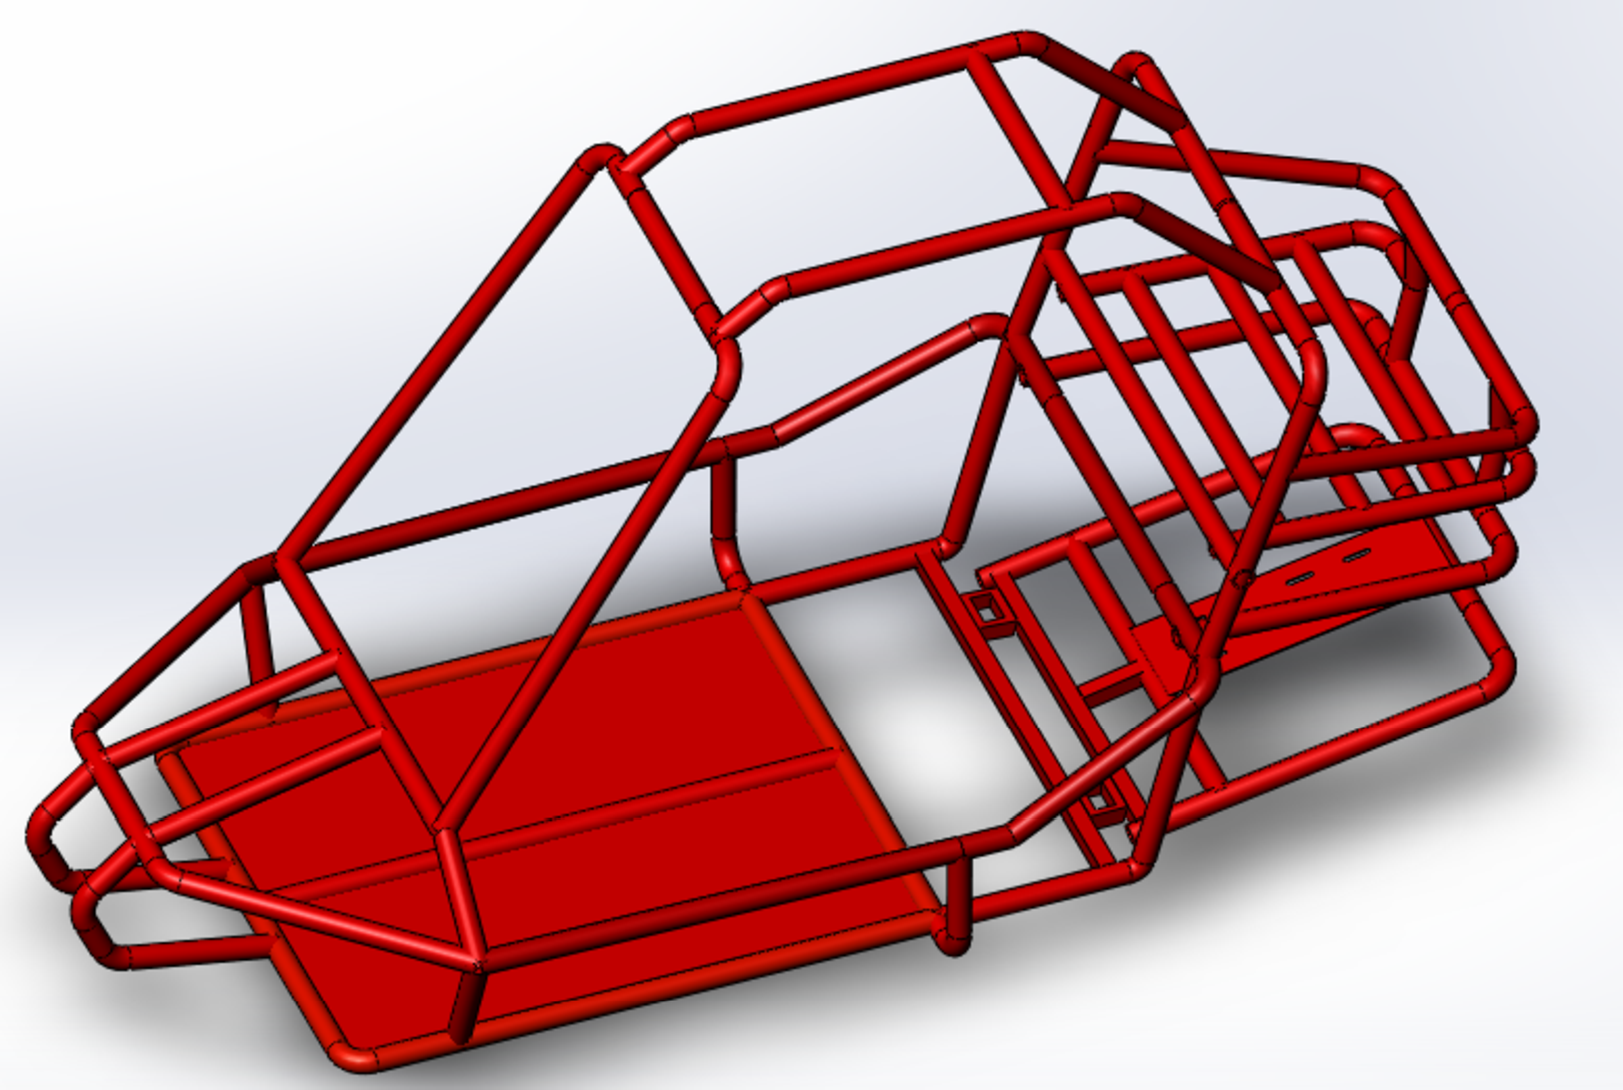
\includegraphics[width=3.5in]{solidwork_model.pdf}
\caption{Initial SolidWorks Model}
\label{solidworks_model}
\end{figure} 

\subsubsection{Controls}
In order to implement the control system necessary for this project, an initial top level block diagram was created.  This block diagram would provide an outline that would guide the design of the control system.  In order to properly control two separate electric motors, it was determined that inputs from a variety of sensors were needed.  These sensors included various potentiometers to measure the input of the throttle and steering angle, as well as multiple encoders to measure the individual rear wheel speeds.  The initial model was designed in \emph{Simulink} and built on a pre-existing model provided by \emph{MathWorks, Inc.}  The source location for the initial model can be seen in the references section.  The original model was adapted to incorporate the sensors needed as well as conform to a particular control scheme that would meet the needs of the project.  The design of the initial top level block diagram can be seen in Figure~\ref{controlblockdiagram}.

\begin{figure}[!h]
\centering
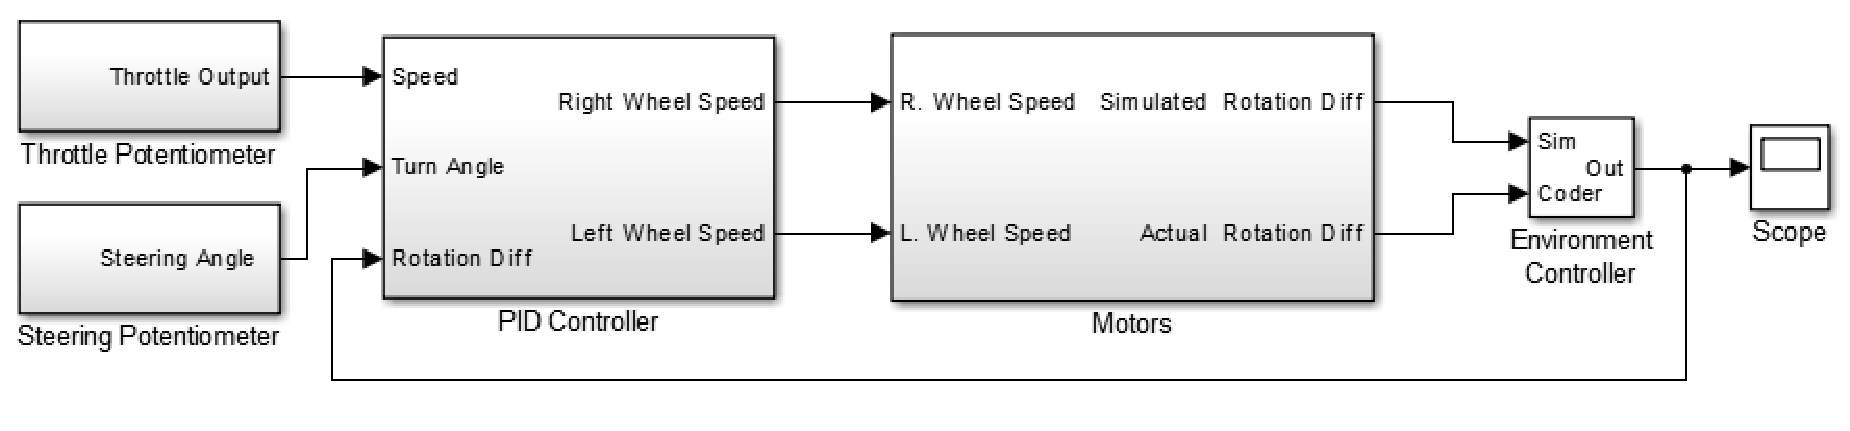
\includegraphics[width=3.7in]{controlblockdiagram.pdf}
\caption{top level block diagram}
\label{controlblockdiagram}
\end{figure}


\subsection{Power Calculations}
One of the first tasks was the calculation of required power to drive the kart. The first step in this process was to decide upon a satisfactory speed for testing the split versus solid axle configuration. After some rudimentary research into standard vehicle performance tests, It was agreed that a maximum speed of twenty miles per hour would be adequate for testing.

	The second step was to gather data about the kart�s rolling resistance. Simulating a fully loaded chassis was done by loading the cart with three people. A linear force gauge was attached to the front of the kart and used to measure the amount of force required to accelerate it to a constant speed. Throughout this process, readings of the force gauge were recorded by video. Several runs were performed to ensure consistent data. A graph from this set of data can be seen in Appendix \ref{initial_horse}.
	
	The rolling resistance data gathered were then used to calculate minimum power requirements. Several estimations were made including frontal area of the kart, final vehicle mass, and a drag coefficient. Calculations showed that a minimum of $1.25$ horsepower was required to maintain a 20 mile per hour speed on flat ground, under the ideal assumptions made. For the same assumptions and a $10\%$ grade, $3.35$ horsepower was required. These calculations were utilized in finding a pair of motors that suited the project requirements. 

	 A spreadsheet containing calculations for power requirements on both a $0\%$ and a $10\%$ grade can be seen in Appendix \ref{power_req}.

\subsection{Budget}	
	In order to successfully complete the project, a variety of parts were needed.  The parts needed by the senior design group consisted of parts to build or repair a chassis, items for safety implementation, the core drive-train equipment, various sensors and microcontrollers needed for the control system. The senior project was allocated a budget of two thousand dollars. 
	
During the first phases of the project, it was decided that the budget would be partitioned into sections including the motors, motor controllers, sensors, and chassis construction or repair. After some preliminary research and projections of total cost based on similar projects, it was apparent that the parts required to build the proposed system would not be easily obtained under the budget cap.  This meant that many parts would have to be acquired through donations and discounts.  After the successful acquisition of a chassis, motors, controllers, and a couple of batteries from donations, many of the remaining required components were obtainable given the budget constraints.  
%////////////////////////////////////////////////////////////////////////////////////////////////////////////////////////////////////////////////////////////////////////////////////////////////////////////////////////////////////////
% DESIGN IMPLEMENTATION
%////////////////////////////////////////////////////////////////////////////////////////////////////////////////////////////////////////////////////////////////////////////////////////////////////////////////////////////////////////
\section{Design Implementation}
\subsection{Overview}

	First, the design had to undergo a significant amount of mechanical modification.  The chassis that the team had donated was in a state of disrepair from the beginning.  The frame was bent, and to retrofit the electric parts onto the kart was no small task.  
	
	The electrical systems had to be configured to include the three twelve-volt batteries in series and then use them to power the motors and controllers.  A schematic provided with the motor controllers was used to aid in this process.
	
	Lastly, the differential motor control scheme was implemented with an Arduino microcontroller.  Using the \emph{Arduino Integrated Development Environment}, code was written that takes inputs from the various sensors and sends outputs to the motor controllers.  The control scheme uses potentiometer readings and encoder values to feed algorithms that were designed to differentiate the wheel speeds.  The controller uses the computed values to send throttle input back to the motor controllers to control the wheel speeds. 

\subsection{Mechanical}
\subsubsection{Chassis}

	The steel chassis used for the electric vehicle was modified from a gasoline powered go-kart originally designed for children.  A drawing of the frame is depicted in Figure~\ref{chassis_model}. When it was donated, it was discovered that some of the components had been damaged and needed to be repaired or replaced.  These components included the shocks, steering column, rear axle and much of the front suspension. In addition to these repairs, chassis modifications were required to accommodate an electrical control system.

\begin{figure}[!h]
\centering
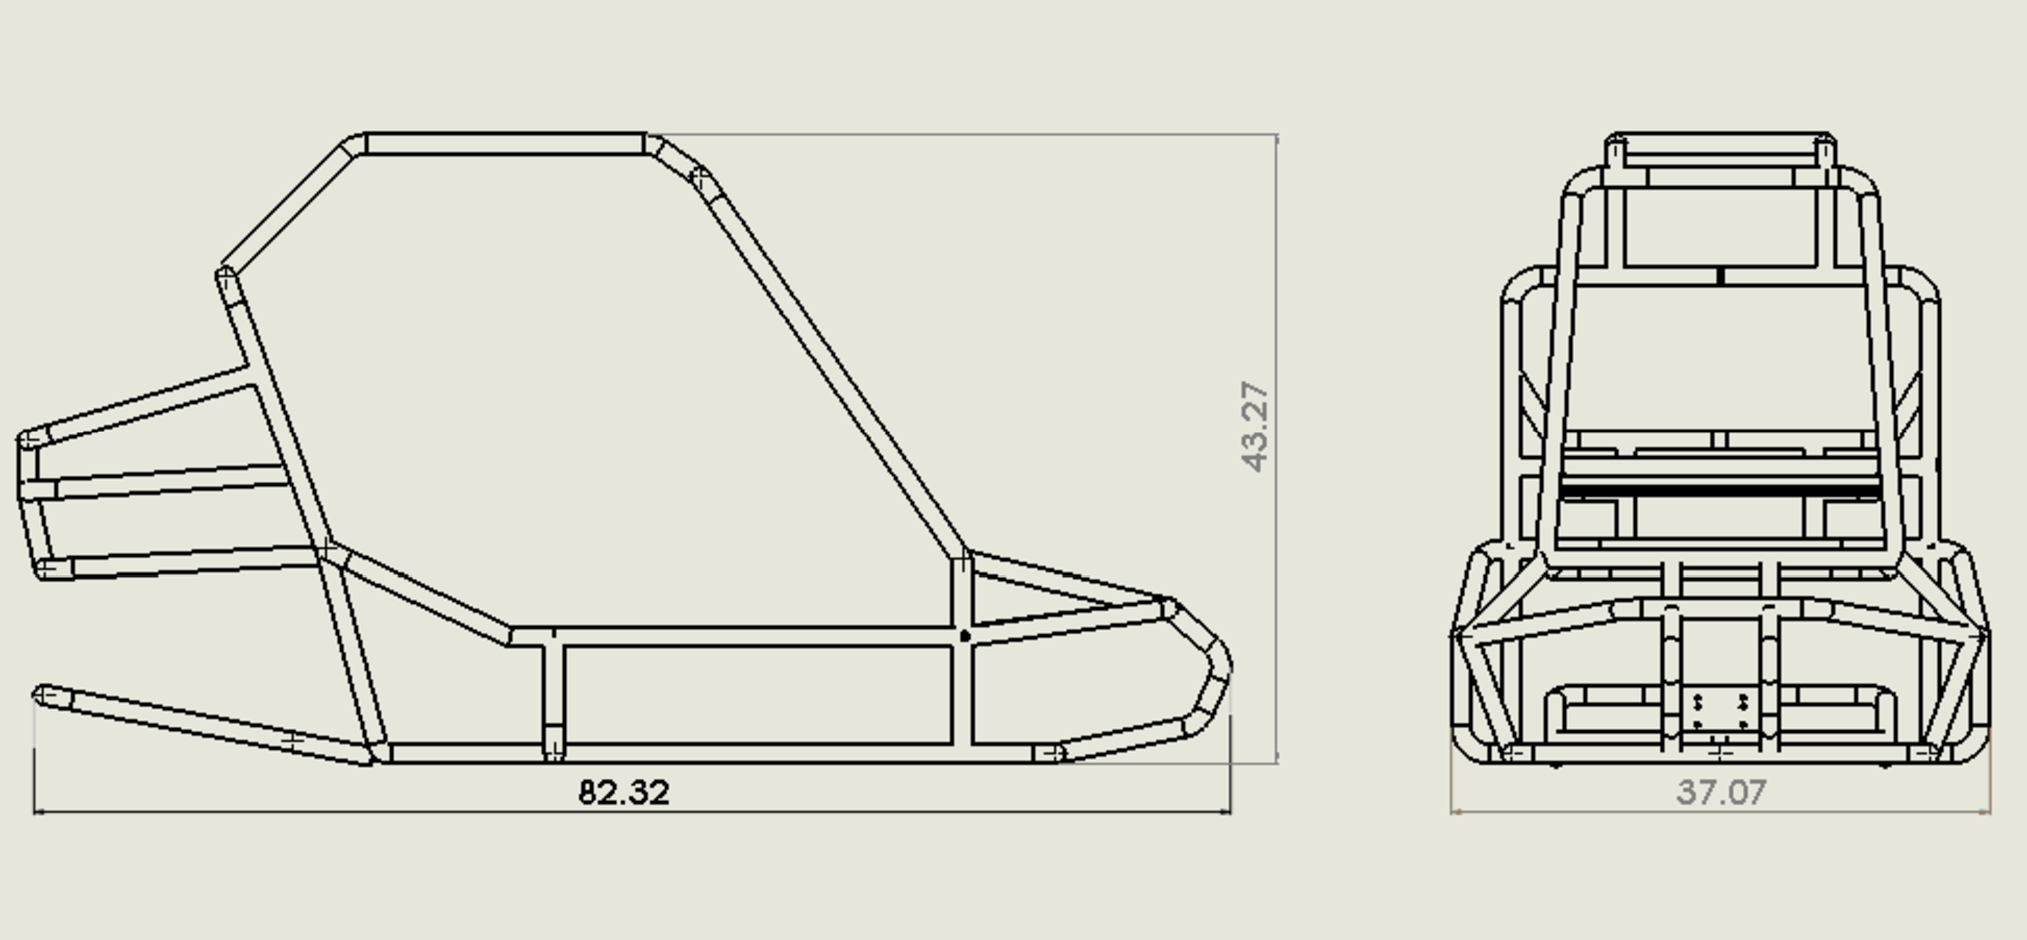
\includegraphics[width=3.5in]{chassis_model.pdf}
\caption{Side and Front View of Chassis}
\label{chassis_model}
\end{figure} 

	The chassis' main modifications were driven by the need to repair broken parts and to provide places to retrofit parts.  The first major repair that was made was altering the rear axle.  The rear of the kart was bent and had to be straightened before splitting the solid rear axle and reattaching it with new bearings to support the cut ends.  Also, the kart was subjected to the tightening of the suspension and steering.  The damaged steering links were replaced and the column eyelets were tightened to eliminate wheel play. This resulted in increased physical control and maneuverability of the kart, as well as a better platform for the steering angle sensor.  These steering modifications also worked to provide better accuracy in test repetitions, as it had less play and could hold more consistent turns.

	After repairing and improving the suspension and steering, the kart was fitted with mounts for a battery box and for the controllers.  The bench seat was removed and replaced with a single seat to make space for the additional hardware components, especially the battery box.  Batteries were secured in the space to the right of the driver's seat.  Structural members were welded to the floor to support the additional weight of the batteries.  In addition, stronger shocks were installed to replace the broken ones and to support the extra weight associated with an electronic control system.
        	
        	Lastly, a shield of Plexiglas was installed between the driver's back and the high voltage components to increase the safety for the driver. Later, a wooden shield was fabricated to cover the top of the high voltage components to protect them from debris and to provide a platform on which laptops could be rested whilst programming and testing in the lab.  Details on the modifications made can be found in their respective sections below.
	
\subsubsection{Rear Axle}
	
	To prepare for the differential control of the wheels, the solid rear axle that came with the kart was split into two pieces.  The method of securing wheels and sprockets on the axle employed a key-way and notches in the items being mounted on the axle.  The existing key-way was extended across the entire length of both sections of the axle to prepare for mounting more items on it.  Extending the key-way made it much easier to position and attach the drive train components.  These components included two sprockets for a dual-motor chain drive system, pillow bearings and a coupling that allowed for a solid or split axle configuration.  One of the sides had to be straightened with a press to repair pre-existing damage from bending of the axle. The chassis also required modification to support the newly split axle. To account for this, the frame was extended downward along the center platform above the axle by means of two plates spaced out by steel rod standoffs and then welded together.   Bearings were then attached to the newly added plates and the cut ends of the axle were inserted into the new bearings. 

	Despite the initial attempts to fully support the split axle halves, they experienced shifting when subjected to hard cornering forces.  The shifting was eliminated by adding screws that passed through bearing collar set screw holes and directly into the axle shafts.  These screws acted as a shear pin to resist the axial loading that is applied to each axle while turning, thereby preventing lateral axle shifting inside the bearings.  
	
\subsubsection{Front Wheels \& Suspension}

	The front of the kart came configured with an A-arm style suspension system.  The system employed two arms pinned to the frame that could rotate in the x-z plane (assuming that the ground is the x-y plane with the y axis running from front to back of the kart).  The front wheels were then mounted to these arms by way of a kingpin (oriented along the z-axis).  Originally, the wheels sagged inward due to the mount holes being worn out by the kingpin that results from strenuous use.  This was fixed by welding on machine bushings to both ends of the mounting tube and replacing the kingpins with steel carriage bolts.  
	
	The shocks that came with the kart needed to be replaced as well.  One of them was bent and disallowed movement in any direction, rotational or compression.  In addition to the one shock being broken, all of them were underrated for the projected weight of the modified vehicle.  They were also repositioned in the front of the vehicle to help with the camber and toe angles caused by the A-arm suspension.  The new shocks were chosen because they are rated to support $730$ pounds of load compression each, and three inches of compression length.  

\subsubsection{Steering Column}
	The steering column needed repairs due to being sloppy and bored out at the mounting holes.  The original tie rod was bent and had to be completely replaced, and the holes were tightened to clean up the some of the play.  Machine bushings were welded to the mount holes here as well, to tighten them up. 

	After tightening up the steering as much as possible, the steering column was chosen as the most reliable place to take a reading of the steering angle.  Because of this, a potentiometer shaft was inserted into the steering shaft and the body of the potentiometer was secured to the chassis.  The potentiometer acts as the sensor and was chosen for its simplicity, ease of coding, and modest expense.  Originally the column was a flat-ended, solid steel rod.  Using a lathe, a hole was drilled into the end to accommodate the adjustable shaft of a potentiometer.  A mounting bracket was fabricated to hold the potentiometer in place as the steering column rotates, and to reduce the axial and shearing stresses acting on it.  The potentiometer shaft was then centered and tied into the steering shaft with a set screw such that it rotated in response to the steering column.   

\subsubsection{Seat}
	
	The original seat in the kart was designed for two passengers.  However, it was decided early in the design process that the second seat needed to be removed to create space for other components.  In addition, with the original seat, drivers who were taller than about $5$ feet and $7$ inches could not operate the vehicle.  Both of these issues were resolved by installing an alternative seat.  The new seat was made from a plastic, cloth, and foam portion of a standard school chair without the stainless steel legs.  The new design used the runners from the old seat to adjust the height so that taller people could operate the kart.  Using the original runners also allowed the vehicle to still make use of the original seat belt. 

\subsubsection{Battery Box}

	The most significant addition to the kart, in terms of size and weight, are the three 80 lb batteries required to power the motors and controllers.  Several accommodations had to be made to safely accommodate the batteries when installing them on the kart.  A steel battery tray and wooden box were fabricated to secure the batteries from sliding around and to protect the driver from any potential malfunctions, meltdowns, etc.  First the passenger side of the kart was modified to support the extra weight of the batteries by welding cross members to the tube steel which ran lengthwise down the kart.  The battery tray was then constructed of L-channel steel and welded to the chassis on the cross bar supports.  The box was constructed of plywood and had a hinged door on the top for battery access.  The location of the battery box was chosen such that it would minimally affect the center of mass (the calculations for the center of mass are in Appendix \ref{B4}).
	
The weight of the batteries and battery box essentially replace, and possibly double, the weight of the second passenger in the old seating arrangement and places the center of mass three inches to the right of the true center.  Placing the box beside the driver also allowed it to serve as a mounting platform for the control panel and arduino housing.
	
	
\subsubsection{Motor Mounts}

	The motors obtained for this project were electric DC motors meant for a golf-cart.  They were designed to bolt directly into a mechanical differential in the rear of the golf-cart.  Because of this configuration, they required motor mounts to be designed and built that would eventually accommodate a sprocket mounted near the face of the motor. The size of the motors, position on the kart, and a mechanism for tightening the chain were all considered in the mount design. Because the motors were designed to bolt directly into a mechanical differential, the  housing was used to provide support for the front of the motor and to cover the armature windings. Taking this into consideration, the motor mount design included a front motor plate which could both secure the motor, cover the windings and provide support for the output shaft on which the sprocket was mounted.  The drawing depicting the design of the motor and its mount can be seen below in Figure ~\ref{motor_solidworks}.


\begin{figure}[!h]
\centering
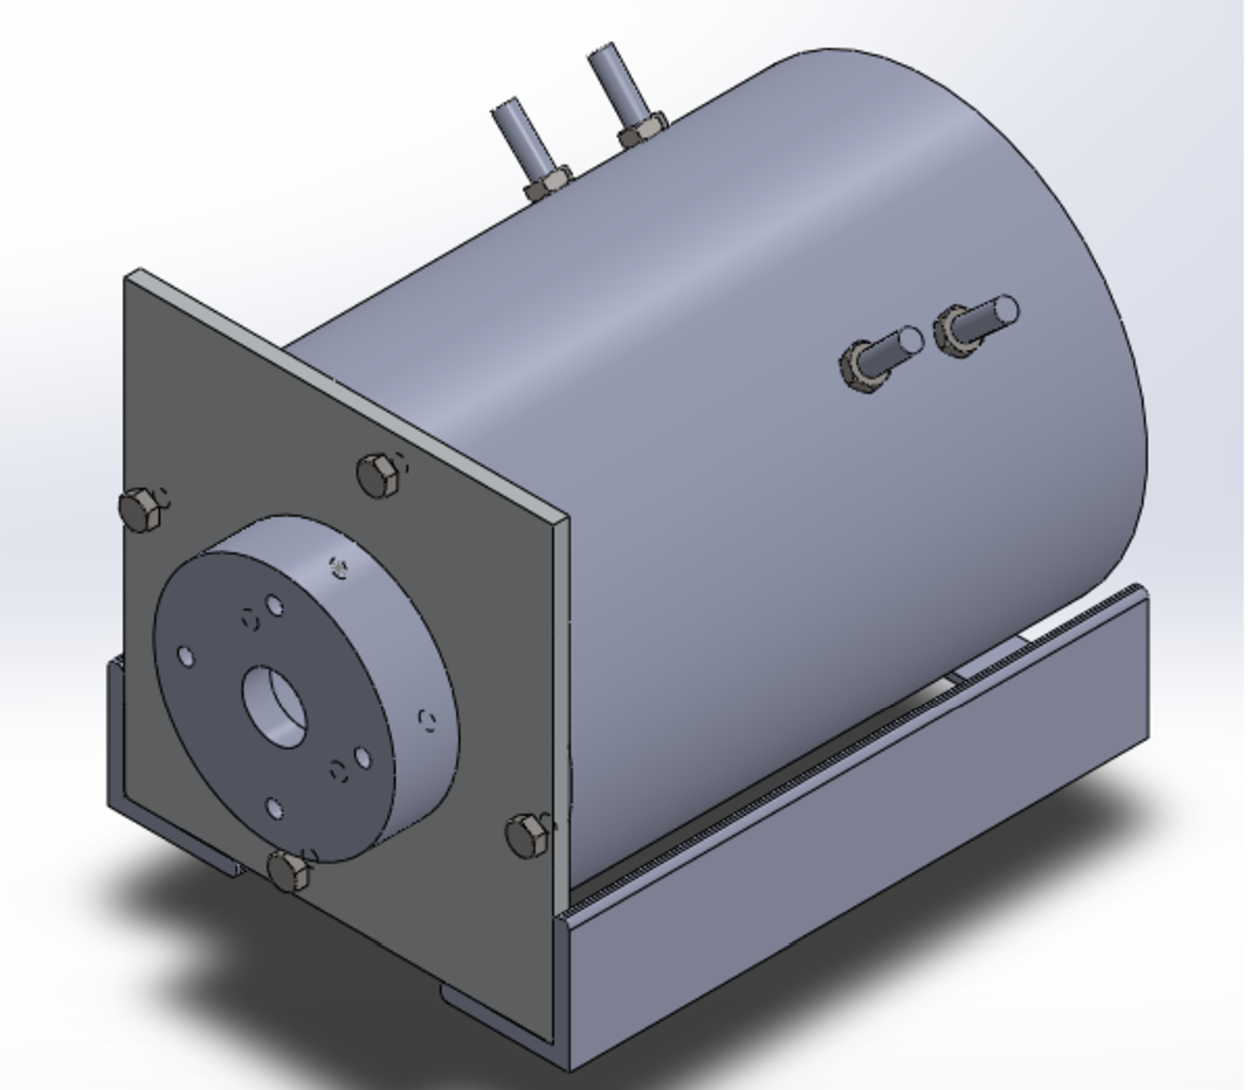
\includegraphics[width=3.5in]{motor_solidwork.pdf}
\caption{SolidWorks Design of the Motors}
\label{motor_solidworks}
\end{figure} 

	The motor mounts were constructed from four separate pieces.  A front motor plate was cut from 1/4 inch steel and drilled to accept the motor and bearing cap mounting bolts.  The second and third pieces were a pair of 3/16 steel angle iron that were welded to the front plate and ran along the length of the motor.  These pieces of angle iron served as the medium for the oblong mounting slots that allowed the whole bracket to slide, thus solving the chain tensioning problem.  The final piece of the bracket was a small iron cross member welded across the back of the angle iron to provide more support to the whole setup.  Once welded together, the motor was mounted to the faceplate using allen head bolts.  In addition to the holes for the motor mount bolts, the face plate was also drilled and tapped to accept bolts that held an aluminum bearing cap.  The bearing cap is described in more detail in the next section.
	
\subsubsection{Output Shaft \& Bearing Caps}
	Because the motors used in this project were designed to be attached directly to a mechanical differential it was necessary to find an alternative means to distribute the power.  Normally, bolting directly to the differential meant plugging the motor onto a shaft built into the device; however, in this design?s particular condition, the motor needed to be fitted with a free standing shaft that could be made to accept a sprocket for a chain.  The necessary component for this process was a nineteen tooth output shaft that normally connected the motor to the gear train of the differential unit. The original shaft had a toothed section that interfaced with those gears.  The shaft also had a stepped end that fit into the motor socket and had bearings at both ends. 

	The bearing on the free end of the shaft and the toothed section that normally interfaced with the differential weren?t needed for this design.  The teeth of the gear were turned down using a lathe and a keyway was milled into the turned down section to accommodate the sprocket necessary for a chain drive configuration.  This solved most of the problems associated with the output shaft, but there was still the problem of how to keep the shaft held into the motor.  This issue was addressed by designing and machining caps to fit over the bearing at the motor end of the shaft and hold the shaft into the motor.  The bearing caps were also designed to prevent any driveshaft movement from axial forces (pushing or pulling on the shaft).  The bearing caps were machined out of aluminum and were drilled to bolt to the faceplate of the motor mount. 

	Issues arose when the central openings in the bearing caps caused binding on the shaft because they were turned down with too low of a tolerance for non-rotational movements in the shaft.  The restriction of deflection at the free end of the shaft, caused by low machining tolerances, in turn caused the shaft to severely rub against the aluminum caps when loaded with the moment caused by the chain tension.  The resultant binding was relieved by boring out the bearing cap openings to higher tolerances.  Also, it was found that the bearing area of the caps was bored out too deeply and with too large of a diameter.  Bushings were added to the caps, taking up the excess depth and allowing the bearings to be pressed into the caps harder and preventing the bearing from moving along the shaft within the cap.  In addition to the bushings, small shims were added between the outer shell of the bearing and the inner circumference of the cap to tighten up the bearings against the cap.

\subsubsection{Chain Drive}
	
	In order to transfer torque from the motors to the wheels, a chain drive system was used.   Number forty roller chain with a single strand working load of $810$ lbs was chosen due to the relatively large amount of torque ($30$ ft-lbs each) output from each of the motors.  To reduce the overall stress on the system and to allow for the differential control of the wheels, one chain was used for each motor.  A pair of sprockets keyed to the motor output shaft and axle shaft, respectively, were implemented to engage the chain system.  As mentioned previously, chain tensioning was implemented through the use of sliding motor brackets.  Once moved to create the desired tension, they were secured to the frame with a set of bolts.
	
	Choosing a gear ratio was a process that required some experimentation.  It was first decided that a ratio of $10:1$ would be adequate for testing.  This ratio was chosen because it would allow to the motors to turn at maximum speed when the kart was traveling twenty miles per hour.  After searching for parts, it was discovered that the sprockets needed to create this ratio were not available for the axle.  There was also concern that this high of a ratio might create too much torque.  It was then decided that a $2.66$ ratio would be easier to implement due to the smaller sizes of the sprockets, and the availability of the parts.  This setup; however, caused the motors to draw too much amperage at startup, failed to provide enough torque to provide adequate acceleration or hill climbing ability and allowed the kart to achieve borderline dangerous speeds.  Finally, a $5:1$ ratio was settled upon. This ratio gave the best balance between top speed and acceleration that was feasibly implemented with available parts. 


\subsubsection{New Pedal (Throttle)} 
	
	The original throttle system for the kart was not suitable for the project.  Its original purpose was to pull a rod that ran from the pedal to the rear of the kart where the throttle cord was attached to the motor.  In addition to being an unsuitable configuration to accept a throttle sensor, the amount of freedom concerning side to side motion of the pedal was unacceptable for the potentiometer sensor that was going to be installed.  In response to these problems, the rod running to the rear of the kart was scrapped, the pedal was removed from the kart and a new configuration was designed to clean up the side to side motion while also accepting easily a potentiometer as a sensor.  A drawing of the proposed configuration is shown below in Figure ~\ref{throttle_pedal}.

\begin{figure}[!h]
\centering
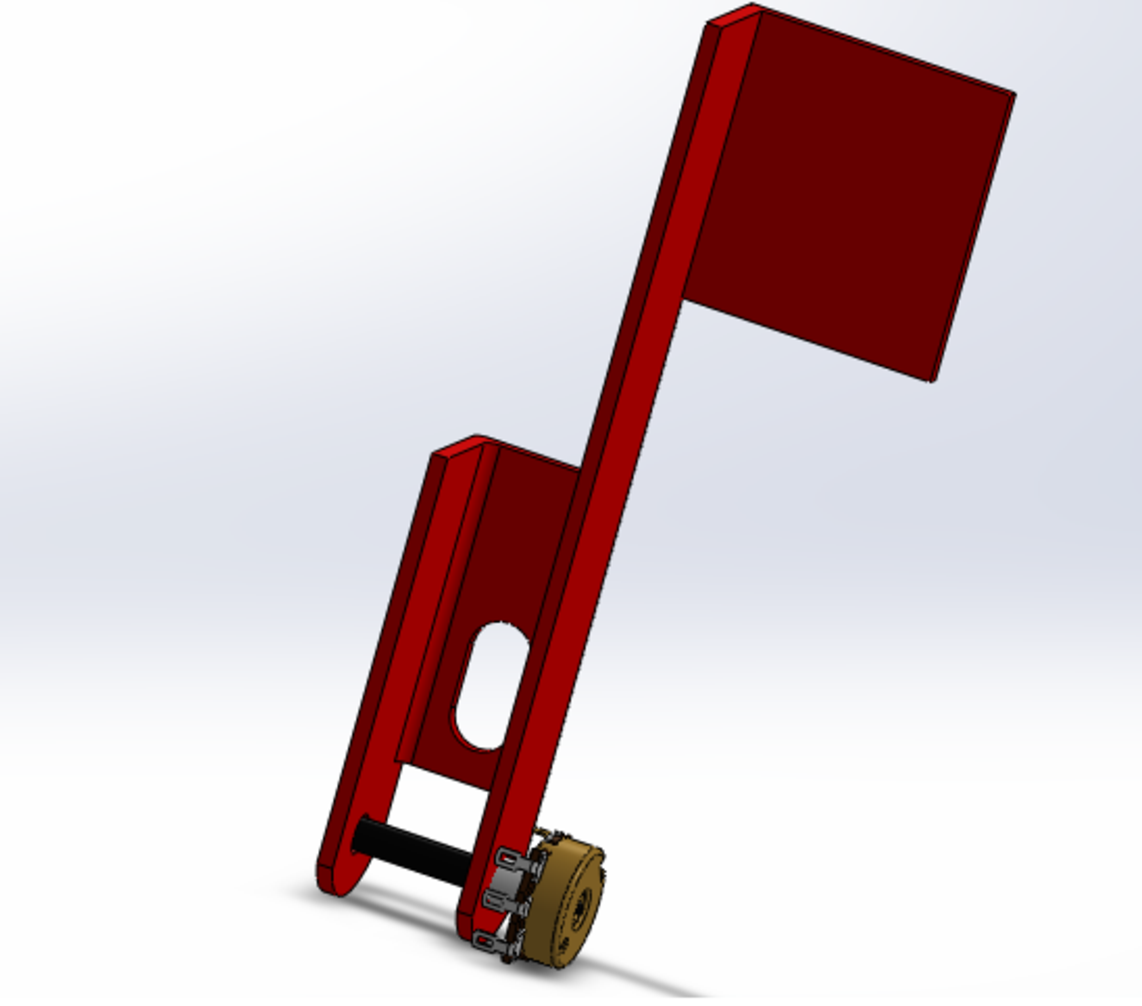
\includegraphics[width=3.5in]{throttle_pedal.pdf}
\caption{Throttle Pedal}
\label{throttle_pedal}
\end{figure} 

	The new configuration consisted of a pedal mount that was fabricated from a piece of steel square bar and angle iron.  The pedal was detached from the old setup and then secured to the square bar with a copper pin, acting as the axis of rotation, was secured into the slot that the pedal rotated about.  Finally, the copper pin was coupled to a potentiometer shaft.  When the pedal was pressed, it rotated the copper pin, which in turn rotated the potentiometer.  This acted as a throttle sensor.  Also included in the new configuration was a more powerful tension spring as opposed to the compression spring originally on the kart.  The new spring provided more force to return the pedal to its original position.  The new configuration was mounted on the floor pan next to where the original setup was mounted.
	
\subsubsection{Brakes} 
	
	Originally, a single brake drum with a cable actuated band was installed on the kart.  Due to the splitting of the live axle, this setup only provided braking on one side of the kart.  To solve this, another brake drum and band were purchased and installed on the opposite side of the kart for additional safety and stability whilst braking.  Immediately after installing the complimentary setup, when comparing the two brakes, it was noted that the original brake drum wasn?t as effective as the new one. The original brake drum was replaced to create uniformity.

	A couple of issues arose during the implementation of the new braking system.  The issues needed to be addressed to let the brakes act in unison.  While the original brake cable worked fine for the old brake, there were no parts available from the manufacturer to actuate the new one. In place of the OEM brake actuation cable, a motorcycle brake cable was used.  It had the sufficient length and strength required for the system, and was relatively easily obtainable.  A custom bracket was fabricated to connect both brake cables to the rod attached to the brake pedal, allowing both brakes to be actuated simultaneously.  The original rod was replaced because it was not long enough to allow sufficient movement to fully release the brakes. 
 

\subsubsection{Control Panel}

	A control panel was designed that featured switches and connections according to the motor controller schematic.  The panel was required to route wiring to its necessary locations and to house the prescribed operations such as the emergency stop, vehicle on/off key switch, rotary forward/neutral/reverse switch, pedal interlock, and mode selection.  Most of the controls were put in place as per the schematic provided in the motor controller manual; however, the interlock switch was left out and an emergency stop was added.  The emergency stop button enabled the driver to quickly break the connection of the control power to the motor controller, thus disengaging the solenoid and killing power to the motors.  The pedal interlock switch was fed into the appropriate pins of the motor controllers to shut the field current to the motors off when the switch was disengaged, thus adding a secondary layer of safety to the system.  The mode selection was a combination of two switches that allowed for four modes of programmed motor controller operation.  A drawing of the control panel can be seen in Figure ~\ref{control_panel}, and its specific dimensions have been provided in Figure ~\ref{control_diagram}. 

\begin{figure}[!h]
\centering
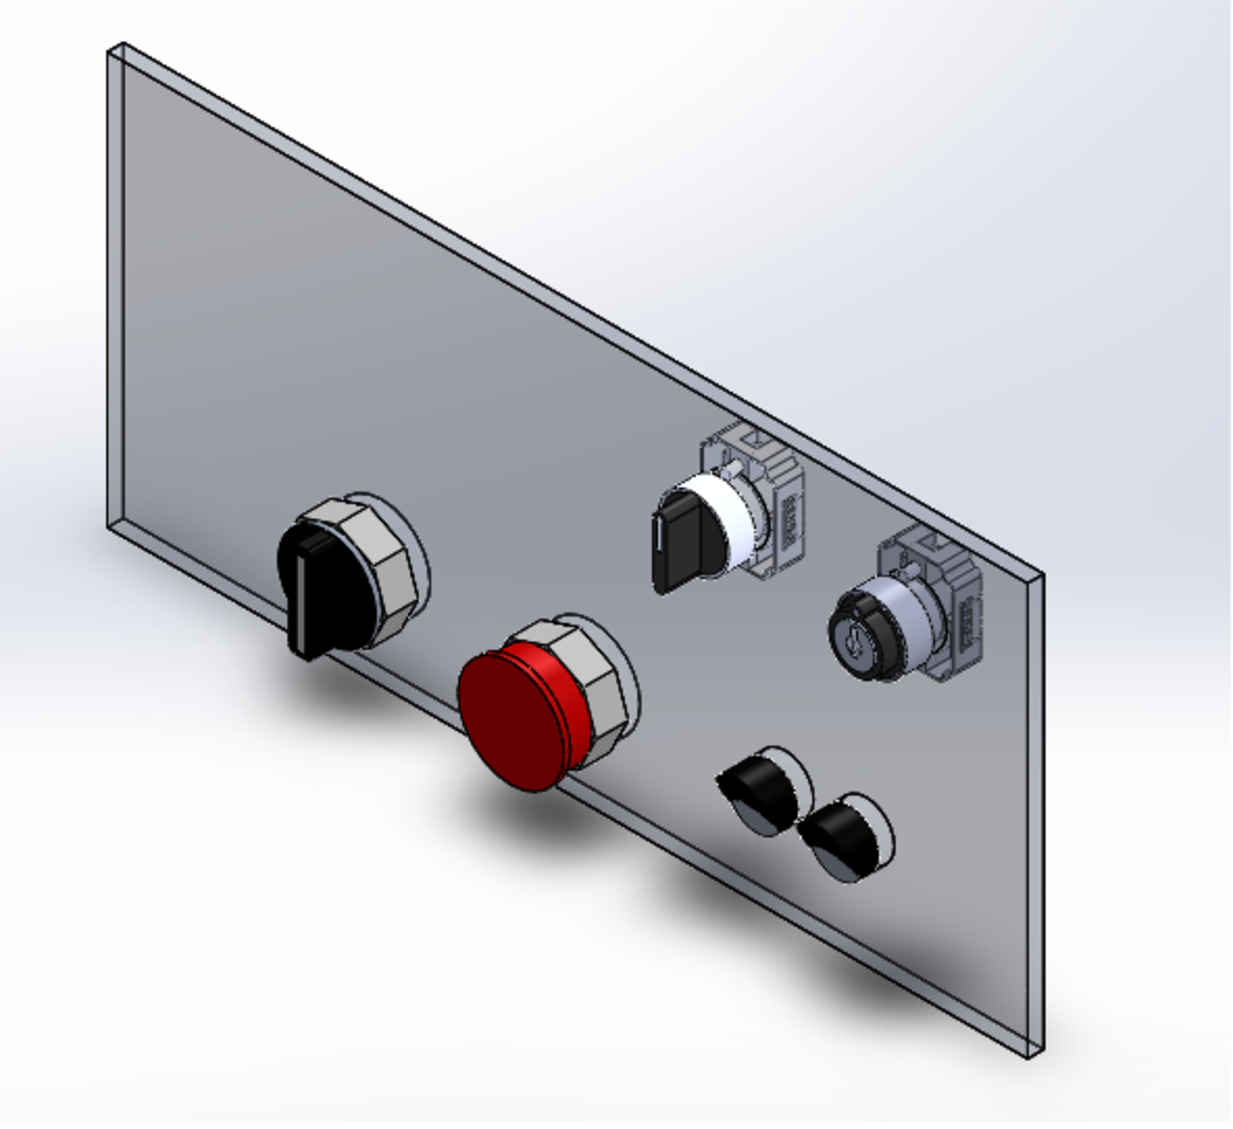
\includegraphics[width=3.5in]{control_panel.pdf}
\caption{Control Panel}
\label{control_panel}
\end{figure} 

\begin{figure}[!h]
\centering
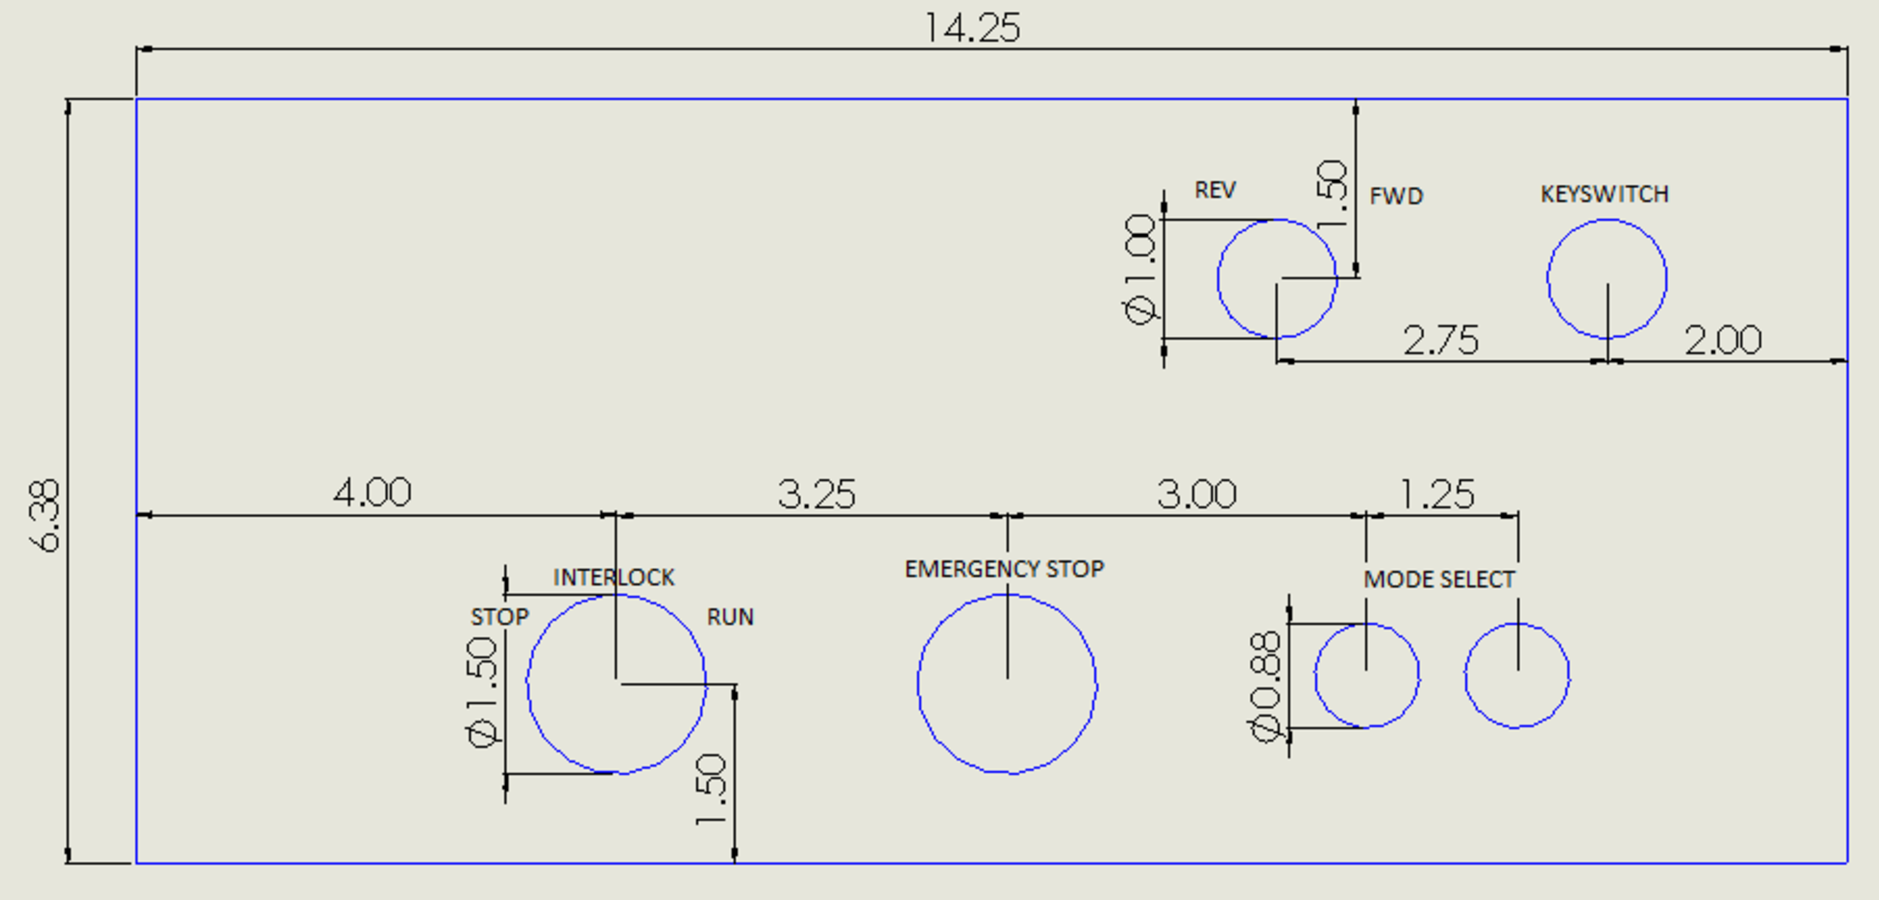
\includegraphics[width=3.5in]{control_diagram.pdf}
\caption{Control Panel Diagram}
\label{control_diagram}
\end{figure} 
	
	The panel was made from plexiglass and was supported with medium sized angle brackets.  It was positioned on top of the battery box at an angle that is efficient for the driver to press the emergency stop button with little effort.  The panel is powered by the 36 Volt battery pack and is hardwired to each controller.  While all main control signals run through this panel, all of the actual signal processing and throttle control is left to the microprocessor.  


%////////////////////////////////////////////////////////////////////////////////////////////////////////////////////////////////////////////////////////////////////////////////////////////////////////////////////////////////////////
% ELECTRICAL
%////////////////////////////////////////////////////////////////////////////////////////////////////////////////////////////////////////////////////////////////////////////////////////////////////////////////////////////////////////
\subsection{Electrical}
\subsubsection{Motors}

	Two $36$ Volt EZ-Go golf cart motors were donated and then taken into Carolina Cars and Clubs to be tested very early in the design process.  Once confirmed that they were both in working condition, attention was turned to finding appropriate motor controllers and batteries to operate them.  A picture of one of the motors is provided in Figure ~\ref{motor_actual}.

\begin{figure}[!b]
\centering
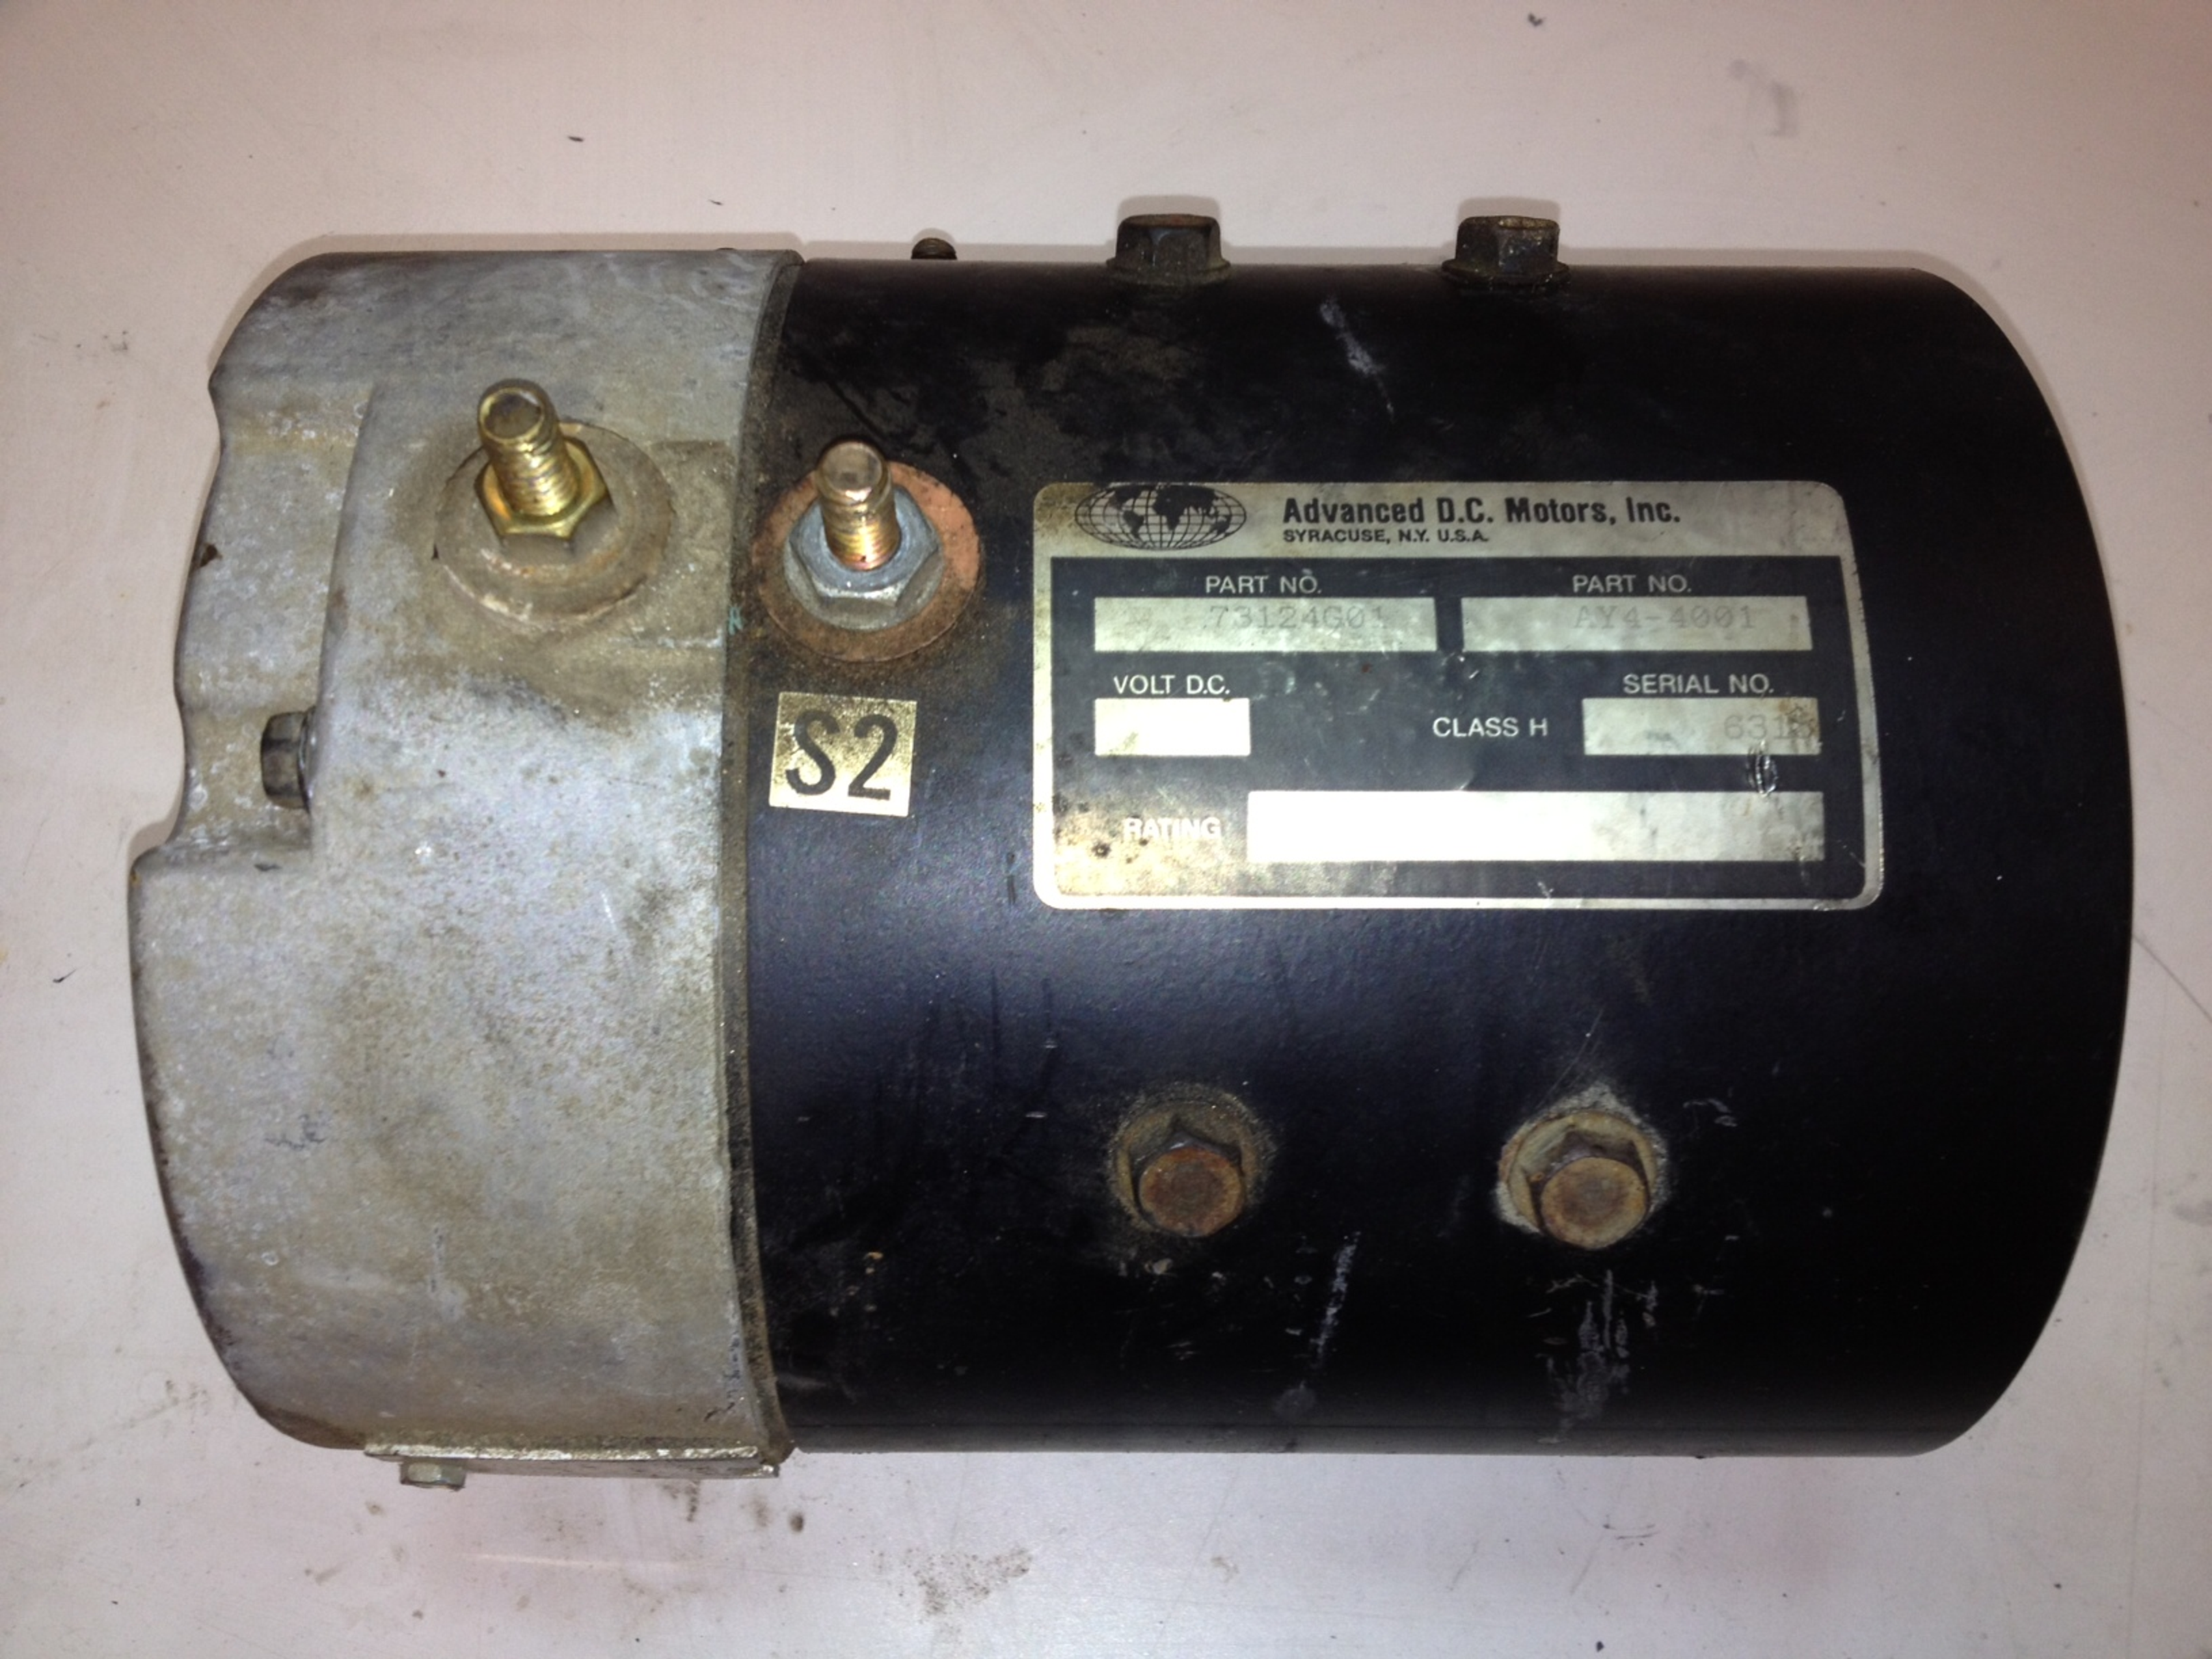
\includegraphics[width=3.5in]{motor_actual.pdf}
\caption{Motor used in Drivetrain}
\label{motor_actual}
\end{figure} 

	The motors produce a fairly flat torque curve with a peak of $30$ foot pounds at startup.  Each motor is capable of drawing nearly $400$ amps. Because they are very powerful relative to what was calculated as sufficient horsepower to propel the kart, safeguards were imposed to limit their maximum output.  The controllers obtained for the motors allow current limiting.  

A torque curve for these motors can be seen in Appendix \ref{motor_torque}.
	
	Other than the mechanical caveats stated above, one motor proved to be quite problematic.  When picking up the motors at the beginning of the project, it was noted that one of the armature windings seemed to be bent slightly out of place, but the team was assured that this would not cause problems.  Late into the project timeline, the motor was acting poorly and the motor controller complained of ``field winding faults.''  Eventually it was discovered that the bent armature windings had rubbed against the field windings during rotation sufficiently enough to tear through the fiber tape holding the field windings and break the winding.  In response to this problem in conjunction with the closing deadline and lack of budget, the team decided to perform surgery on the motor.  The motor was dismounted from the kart and dismantled.  The armature windings that were bent and uncoated were pushed back into place, and an epoxy coating was applied to them to prevent shorting.  The broken field winding was pulled from beneath the tape, ran to the bottom of the windings and soldered back together.  Any exposed field windings were also covered with epoxy and the motor was reassembled.  The motor, upon being reinstalled onto the kart, proceeded to perform appropriately.

Pictures of the deformed and broken windings can be seen in Appendix \ref{broken_windings}.


\subsubsection{Motor Controllers}
	
	The Curtis motor controllers used on the kart were donated from E-Z-GO golf carts based out of Atlanta, GA.  The controllers were donated from a shelf of parts that were no longer getting used at E-Z-GO, and thus were easily repurposed for academic use.  E-Z-GO also donated a manual that included a wiring diagram for the controllers and some general guidelines for programming them.  In addition to the manual, the controllers came with a programming unit that was used to display an impressive amount of data about the controller and motor including throttle percentage, motor currents, voltages, faults in the system and much more.  
	
	The Curtis motor controllers have a wide range of functionality. They can output information such as the voltage and current being supplied to the motors in real time. This was immensely useful when testing some of the control code.  They can also be programmed to set parameters such as a limit on the throttle response or top speed and much more.  The programmable parameters were carefully gone through and values were established to make the motors perform optimally for our proposed system.  The throttle type was changed to accept a ``sensor'' input, which was provided by the Arduino microcontroller.  The acceleration, speed and other performance variables were chosen to run the motors in an acceptable range of current while attempting to get the performance characteristics desired for the differential control.  Additional safeguards were set via the programming unit to account for potential malfunctions, and several system issues were caught using the fault output of the programmer that would have been nearly impossible to diagnose otherwise.
	
	The motor controllers were mounted in the rear of the kart on the rack behind the driver's head.  The mount was fabricated from a large piece of aluminum. Aluminum was chosen due to its light weight and ability to dissipate heat quickly.  The location was chosen such that the controllers would be close to the motors, yet somewhat separated from the driver. In addition to being optimally placed in relation to the motors, the controllers were installed on the top, left rear section of the kart for ease of access for programming.  Being set on the rack provided a great platform to make the controllers accessible, but it also allowed air to move over and under the controllers to increase heat dissipation through convection.  A final perk to the choice of mounting the controllers behind the driver was that their placement helped to offset the right to left influence of the battery weight on the passenger side of the kart.

\subsubsection{Solenoids}

	Two Trombetta Bear P/N 114-3611-010 solenoids were obtained to act as relays that open and close the high current motor circuitry using a low current input.  The low current input is engaged by rotating the key switch into the on position.  This provides control power, low current 36V power, to the motor controllers.  The motor controllers then drop a programmed amount of voltage across the low current side of the solenoids, thus activating the coils.  These bring the metal contacts into place with a magnetic field to close the loop of the high power circuit.  The circuit connecting the batteries to the motor controllers and the motors is initiated by the keyswitch via the solenoids as shown in Figure~\ref{solenoid}.  These particular solenoids are capable of sustaining a resistive or inductive load carry or interrupt of $225$ amps with a maximum inductive inrush capacity of $600$ amps.

\begin{figure}[!h]
\centering
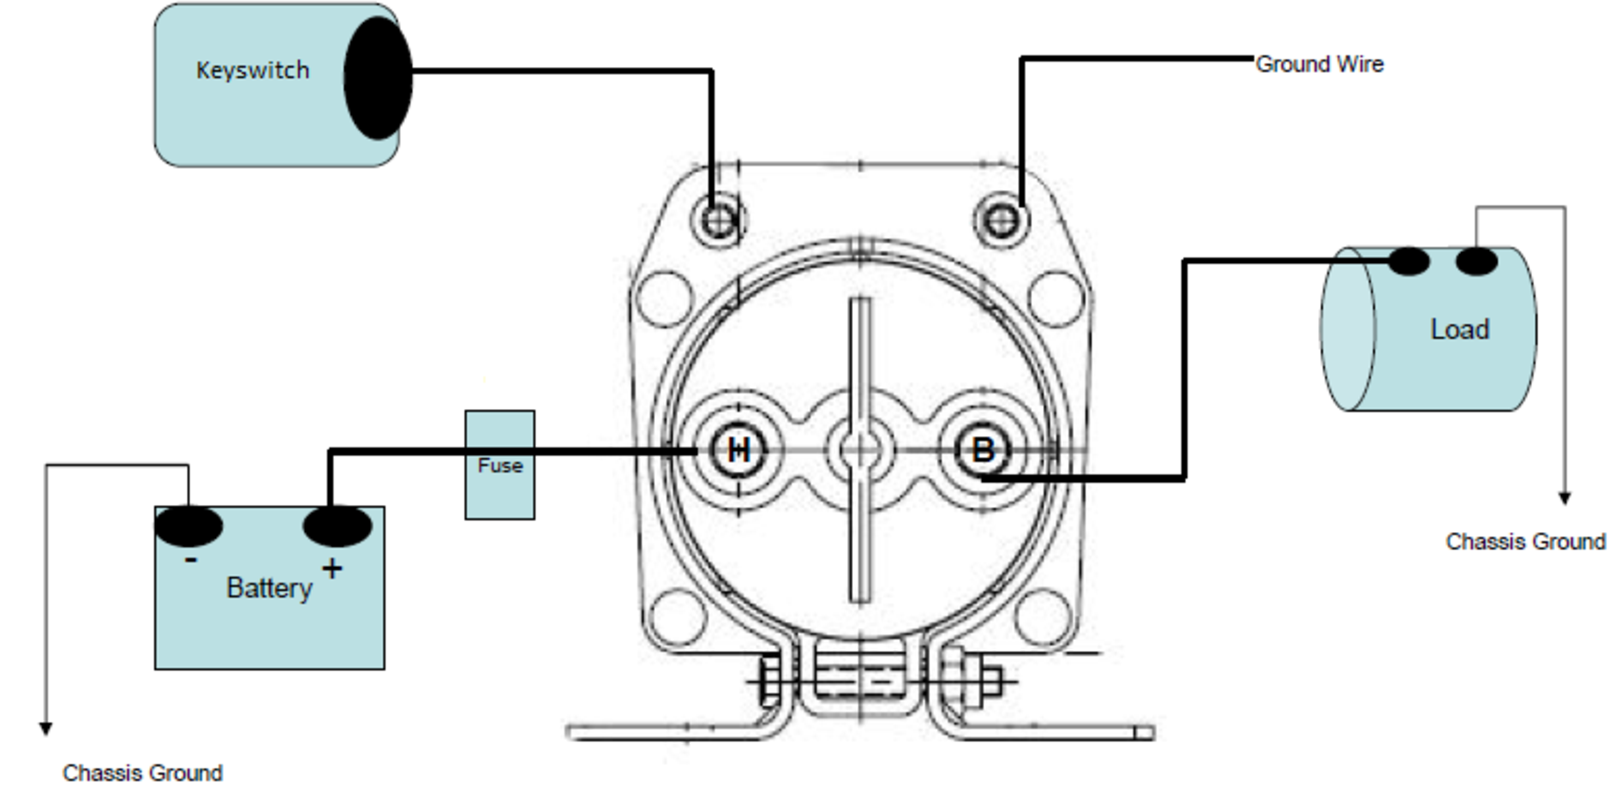
\includegraphics[width=3.5in]{solenoid.pdf}
\caption{Schematic showing connections with the solenoids}
\label{solenoid}
\end{figure} 

\subsubsection{Chassis Ground}
A chassis ground was used in an attempt to reduce the amount of high amperage wiring required in the vehicle.  To implement the chassis ground, studs were welded to various points on the chassis to serve as grounding points.  This allows the ground side connections from each speed controller to be terminated at the closest chassis point, rather than running wire back to the ground battery post.  This also allows the ground side of the battery pack to require only a single point of connection (a short distance from the battery) to complete the circuit.

Initially, both the high amperage and signal circuits were connected using the common chassis ground.  After suffering several issues with noise and interference, it was decided to isolate the signal circuits from high amperage circuits by using  separate grounds. This was accomplished by using a separate power source and ground for the microcontroller and control circuitry which completely isolated the low voltage systems now from the high capacity lead-acid batteries.  The issue of noisy and randomized control circuit outputs was mostly solved by separating the grounds.  It was later discovered that because the motor controllers can accept multiple inputs for a ``type 2 throttle,'' they had a feature to feed voltage on the line that we had connected to ``sensor ground'' between the motor controller and the control circuitry.  This back-feed of voltage into our system was causing throttle issues when the control circuitry was either turned off completely, or turned on after the motor controllers were powered up.  This was solved by turning the control power on before engaging the motor controller power.  This ensured that a ``sensor input'' was provided to the motor controllers on startup to prevent confusion as to the intended input for ``type 2 throttle.''


\subsubsection{Arduino}

Of the many microprocessors considered for this project, the Arduino Du\'e was chosen as the best fit.  Arduino was chosen as the brand of microcontroller because of its high level of support in the engineering and hobbyist community and also due to the availability of pre-developed code and ease of obtaining the hardware.  The Du\'e board specifically was chosen over other Arduino products based on the extensive research and comparisons made between similar products.

There were two major advantages that the Du\'e has over many of the other Arduino microprocessors.  First, the clock speed is set at $83$ MHz which provided one of the highest processing speeds of the initially proposed microprocessors.  Secondly, the Du\'e contains two integrated digital-to-analog output pins, which eliminated the need for an extra component to make the transition between the digital signals of the microprocessor and the analog input that motor controllers require.

There are also two significant disadvantages to using the Du\'e that had to be overcome. The first is that this particular board was still in the ``beta'' phase.  This meant that Arduino had yet to work out all of the bugs in this current model and its IDE.  The second caveat was that the Du\'e's maximum allowable I/O pin voltage is $3.3$ Volts.  This I/O restriction was problematic because many of the commercially available sensors operate with $5$ Volt I/O, which could potentially damage the processor on the Du\'e.  In order to accommodate this problem,  the team put extra care into choosing as many configurations as possible that were easily adapted to $3.3$ Volts.  The throttle and steering sensors were simple potentiometers that could be fed by the Arduino and thus restricting them to $3.3$ Volts maximum.  The encoders posed a challenge, however.  To adapt the encoders to the Du\'e's limitations, the team hooked the encoder input line to the $5$ Volt output pin on the Arduino Du\'e and then employed two-channel voltage level converters to step down the output voltage of the encoder sensors to $3.3$ Volts.
	
Several more problems presented themselves during testing.  One Arduino failed during initial bench testing of some op-amp circuitry designed to modify the output range of the digital-to-analog outputs.  Although an exact cause was never explicitly proven for the failure, it was presumed that a high voltage was encountered while testing the output from the op-amp circuit.  The circuit was later reconfigured to prevent high voltage from being applied directly to the I/O pins of the Du\'e.  In order to prevent damage to other components, a system was then implemented to ensure that circuitry and code were double checked by peers before any serious and potentially dangerous testing was performed.
	
Another issue was encountered during turn radius testing.  A spiking voltage response was received at the Curtis controllers without any user input.  It was determined that this spiking was caused by noise in the system and from varying resistances in the physical potentiometers which fed a mapping function in the throttle-response code.  Due to these causes, the throttle input was falling below zero and negative values were assumed by the microcontroller to represent 100\% throttle.    

Lastly, it was assumed that because of the placement of the Arduino and its housing, that the high current wires running under it could have been causing electromagnetic interference with the sensors and microcontroller.  Originally, the housing for the Arduino Due was milled out of a piece of wood and enclosed with a clear acrylic top so that the inside components were visible.  During testing of the accelerator and steering inputs, it was determined that excessive noise from the potential electromagnetic fields were likely causing the Arduino to send errant outputs to the motor controllers.  Shielded cat-5 cable was utilized to protect the inputs to the Arduino from interference.  In addition, a new box was fabricated out of aluminum to shield the Arduino, $8$ Volt-voltage regulator, and op-amp circuitry from other possible electromagnetic fields.  The box was reattached on top of the battery box next to  the control panel for ease of access and to keep the majority of the wires running along the right side of the vehicle.  For an additional level of protection, the ground node for the Arduino circuit was separated from the ground node of the high-current circuit, as stated before.

When finally implemented, the Arduino Due was powered by a $11.3$ Volt LiPo battery that was run through an 8 Volt regulator.  The 8 Volt regulator supplied the Arduino directly with 7.88 Volts at less than $800$ milliAmps.  The Arduino was wired to accept two analog inputs, one for each potentiometer.  It was wired to also accept six encoder signals, three per encoder and per encoder, two for quadrature rotational pulses and one for a single �absolute� pulse per revolution.  The outputs, DAC pins 0 and 1 were fed to the op-amp circuit, and the $3.3$ Volt and $5$ Volt pins were wired to busses to provide power to the sensors.  Other devices were also connected to the Arduino including two LEDs, and SD card breakout board and a pull-down switch .  A table of pin connections can be seen below.

\begin{table}[ht] 
\caption{Arduino Pin Connections} % title of Table 
\centering
\resizebox{9cm}{!}{
\begin{tabular}{l l l} % centered columns (3 columns) 
\hline\hline \\%inserts double horizontal lines 
Pin & Use \\ [0.5ex] % inserts table %heading 
\hline \\ % inserts single horizontal line 
A10		& 	Steering Potentiometer\\
A11		& 	Throttle Potentiometer\\
DAC0	& 	Throttle output to op-amp for left motor\\
DAC1	& 	Throttle output to op-amp for right motor\\
GND		& 	To ground bus for various applications\\
Vin		& 	Power from the voltage regulator\\
3.3V		& 	To 3.3V power bus to power sensors and the SD card\\
5V		& 	To 5V power bus to power encoders\\
8		& 	LED for general purpose use\\
9 		&	Pulldown Switch\\
10 		&	SD Card signal\\
11		& 	LED for power indication\\
23		& 	Encoder 1 Pin A\\
25		& 	Encoder 0 Pin A\\
27		& 	Encoder 1 Pin B\\
29		& 	Encoder 0 Pin B\\
31		& 	Encoder 1 Pin Z\\
33		& 	Encoder 0 Pin Z\\[1ex]
\hline 
\end{tabular} 
}
\label{arduino_pin_connections} % is used to refer this table in the text 
\end{table}
	
A schematic of the Arduino Du\'e�s pin layout can be seen in Appendix \ref{arduino_pin}.


\subsubsection{Op Amp Circuitry}
	
	During preliminary research into the Curtis motor controllers, it was noted that the required input for a ``type 2'' sensor throttle did not match the stock output for the Arduino Du\'e.  While testing for throttle response, it was noted that the digital-to-analog output voltage range from the Arduino Du\'e was between $0.55$ Volts and $2.75$ Volts, not the $0$ Volts to $3.3$ Volts that the team had anticipated.  This voltage range needed modification before communicating with the Curtis motor controllers.  The voltage range recommended for the motor controllers to perceive a usable input was discovered to be between $0$ Volts to $5$ Volts,  with a possible deadband of nearly $0.2$ Volts and max input of as little as $3.5$ Volts based on the programmed parameters.  This meant that without adjusting the output from the Arduino, the motor controllers would receive throttle input with no actual input from the throttle sensor.  This was due to the minimum output of the Du\'e being higher than the minimum input allowed for the controllers.  In addition, expanding the upper value of the DAC pins gave better resolution to more appropriately operate the vehicle and provide greater control of the wheel speeds given sensor inputs. To remedy this communication error and regulate the voltage range for maximum resolution, a circuit using an op-amp was designed and implemented.  
	
	The following equations and diagrams were obtained from the NCSU ECE-455 class notes and were used to calculate the new resistance values discussed above:
	
\begin{figure}[!h]
\centering
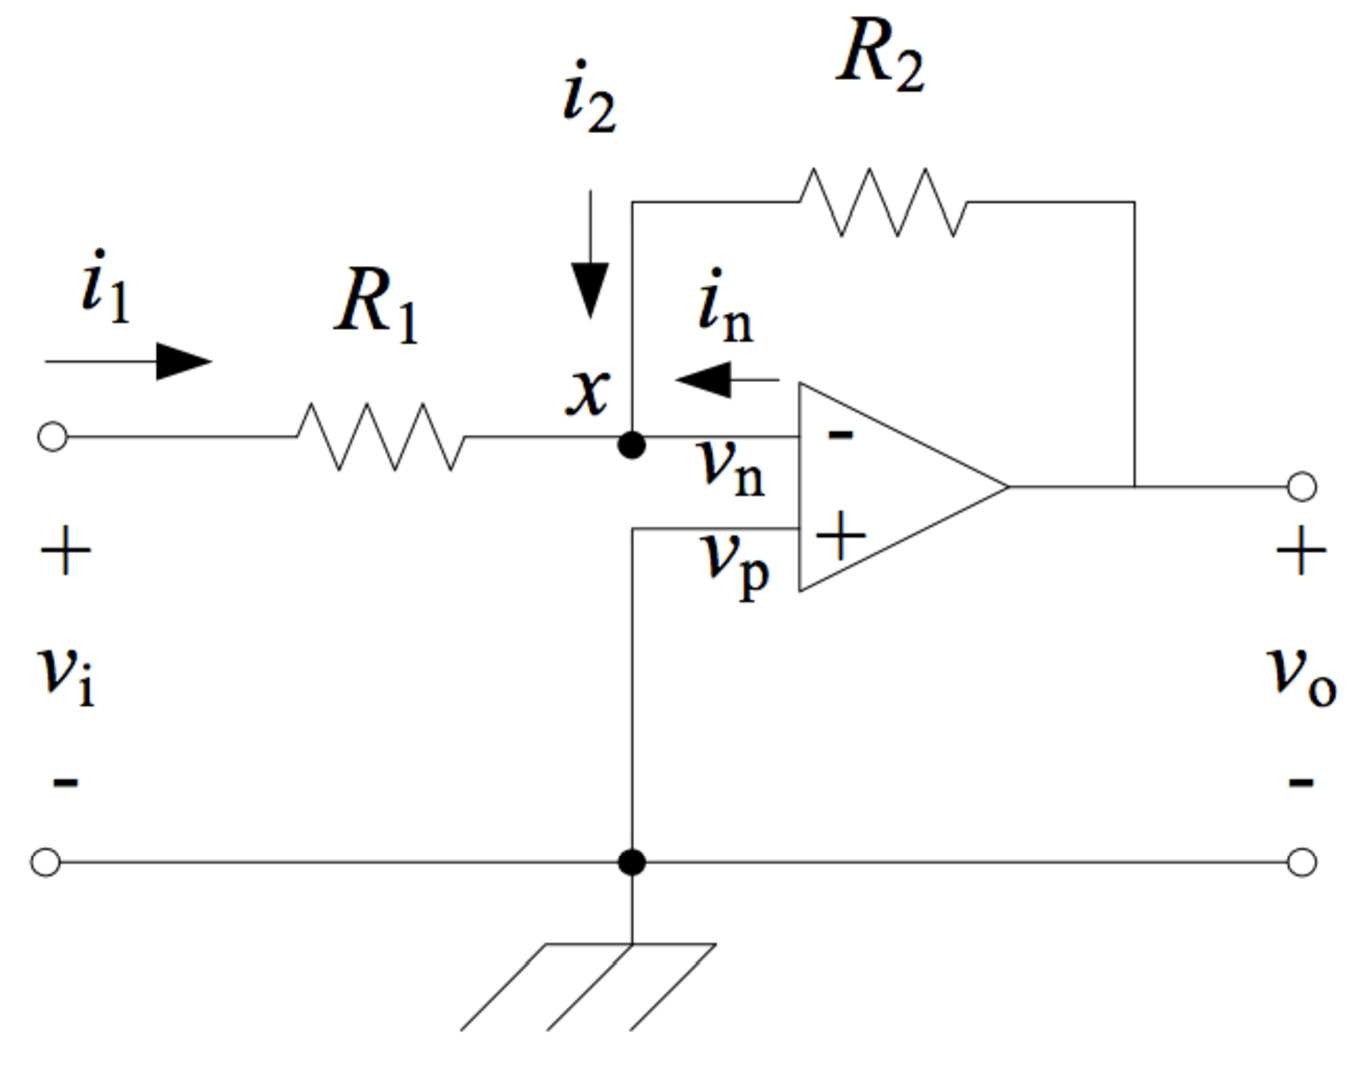
\includegraphics[width=3.7in]{opamp_circuit_1.pdf}
\caption{Inverting Amplifier}
\label{inverting}
\end{figure}

\begin{figure}[!h]
\centering
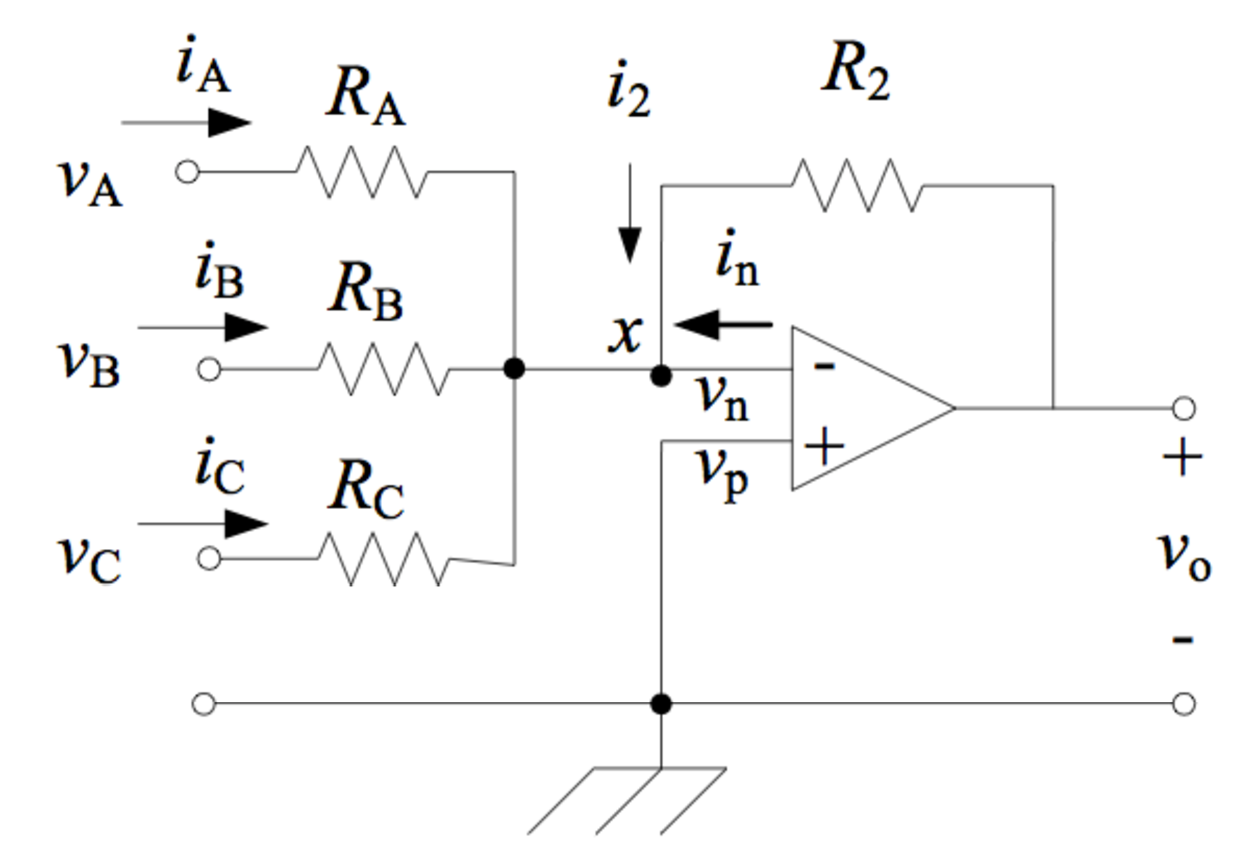
\includegraphics[width=3.7in]{opamp_circuit_2.pdf}
\caption{Summing Amplifier}
\label{summing}
\end{figure}


\begin{equation}\label{vo_vl}
\frac{v_{o}}{v_{i}} = -\frac{R_{2}}{R_{1}}
\end{equation}


\begin{equation}\label{Vo}
V_{o} = -(  \frac{R_{2}}{R_{A}}V_{A} + \frac{R_{2}}{R_{B}}V_{B} + \frac{R_{2}}{R_{C}}V_{C})
\end{equation}

\begin{figure}[!h]
\centering
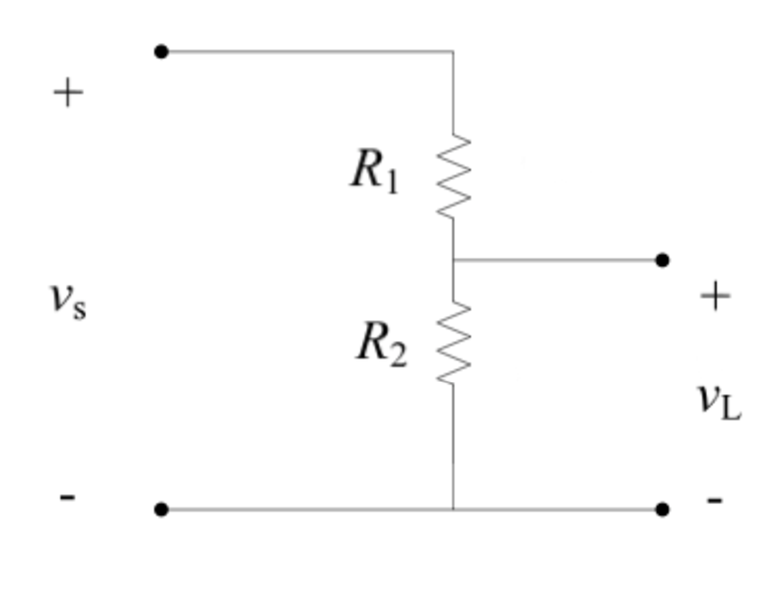
\includegraphics[width=3.7in]{resistor_circuit.pdf}
\caption{Voltage Divider}
\label{resistor_circuit}
\end{figure}

\begin{equation}\label{vL}
v_{L} = \frac{R_{2}}{R_{1}+R+{2}}v_{s}
\end{equation}

	
The op-amp circuit shown in Figure~\ref{opamp_circuit} utilizes two sub-circuits in series to attain the appropriate expansion of the range while also offsetting the minimum voltage outputted.  Shown on the left of the diagram is an inverting amplifier circuit (Figure~\ref{inverting}) utilizing resistors $R1$ and $R2$.  Its purpose is to amplify the maximum output voltage range and, based on this particular configuration, change its polarity.  Shown on the right of the diagram is a summing amplifier circuit (Figure~\ref{summing}), utilizing resistors $R1$ and $R3$.  Its purpose is to subtract a constant voltage from the previously expanded range in order to decrease the minimum output down to the required low end of the range.  The voltage being subtracted was obtained from the voltage divider circuit utilizing resistors $R3$ and $R4$.  Note that the source value for the voltage divider is negative, this was done because the summing amplifier circuit can only add voltages, thus it was necessary to obtain and add a negative value to simulate subtraction.  Together, the pieces of this circuit create a wider voltage range with a closer-to-desired minimum and maximum output voltages.
			
The original values for this were calculated to be:
	
\begin{center}
\begin{tabular}{c c}
$R1 = 510 \Omega$    &    $R2 = 1.15 k\Omega$ \\
$R3 = 2.67 k\Omega$  &  $R4 = 8.2 k\Omega$ \\
\end{tabular}
\end{center}
\begin{centering}
$V_{cc} = 5V$\\[2ex]
\end{centering}

The $5$ volt input was supplied from the Arduino's $5$ Volt output pin. $V_{sig}$ was the Digital to Analog output from the Arduino.  After testing this circuit however, it was found that this particular setup was passing too much current and not providing adequate amplification of range.  To address this, the resistance values were re-calculated to keep roughly the same ratios, but to include higher values in order to limit current more.  The calculations, the slight changes to circuit layout, and the updated values are addressed below.

\begin{figure}[!h]
\centering
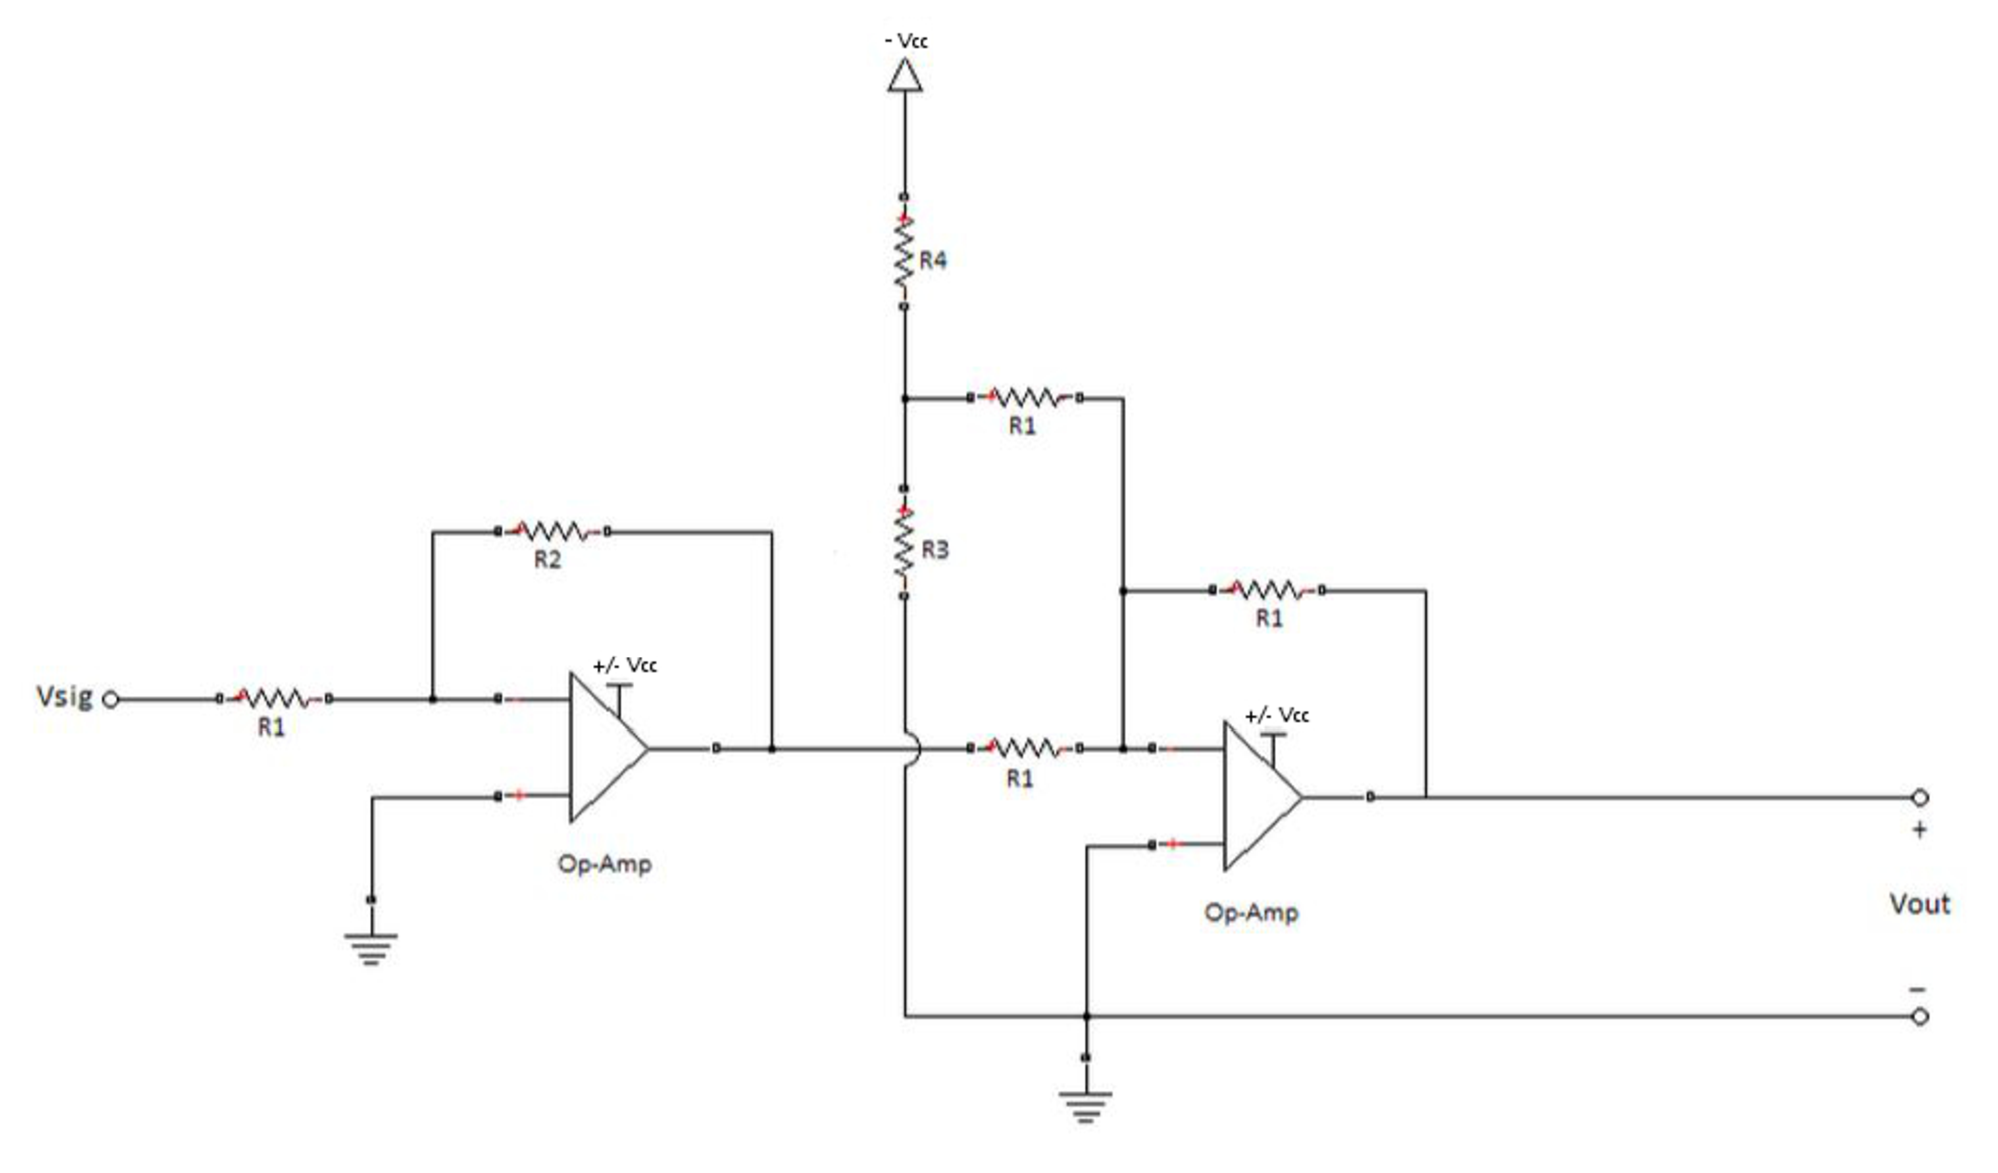
\includegraphics[width=3.7in]{opamp_circuit.pdf}
\caption{Op-amp Circuit}
\label{opamp_circuit}
\end{figure}


Equations~\eqref{vo_vl}, ~\eqref{Vo}, and ~\eqref{vL} from above were manipulated to arrive at the ending values for the resistors.   These equations were combined and simplified to obtain the following:

\small
\begin{subequations}
\begin{align}
V_{out} &= -\frac{R_{2}}{R_{1}} \left( - \left( \frac{R_{1}}{R_{1}} \left(-V_{cc}\left( \frac{R_{3}}{R_{3}+R_{4}}\right) \right)+\frac{R_{1}}{R_{1}}\left(V_{in}\right) \right) \right) \label{4a}\\[1ex]
V_{out} &= \frac{R_{2}}{R_{1}} \left( \left( -V_{cc}\left( \frac{R_{3}}{R_{3}+R_{4}}\right) +V_{in} \right) \right) \label{4b}\\[1ex]
0V &= \frac{R_{2}}{R_{1}} \left( -8V\left( \frac{R_{3}}{R_{3}+R_{1}}\right) +0.55V \right) \label{4c}\\[1ex]
0V &= -8V\left( \frac{R_{3}}{R_{3}+R_{1}}\right) +0.55V \label{4d}\\[1ex]
5V &=\frac{R_{2}}{R_{1}} \left( -8V\left( \frac{R_{3}}{R_{3}+R_{1}}\right) +2.75V\right) \label{4e}\\[1ex]
V_{out} &=\frac{22k\Omega}{10k\Omega} \left( -V_{cc}\left( \frac{820\Omega}{820\Omega+10k\Omega}\right) +V_{in}\right) \label{4f}\\[1ex]
V_{out} &=2.2 \left( - 0.0759V_{cc} +V_{in}\right) \label{4g}\\[1ex]
V_{out} &=2.2 \left(V_{in}\right) - 1.334V \label{4h}
\end{align}
\end{subequations}
\normalsize

Equation~\ref{4a} represents the entire circuit performance from input to output.  To solve for the variables and the resistances, the equation was simplified again.  The simplification of equation~\ref{4a}  yielded equation~\ref{4b}. 

This equation was then given a few boundary conditions including the lower range bounds of the input and output, the upper bounds of input and output, and the projected $V_{cc}$ voltage to be applied to the circuit.  Previously, the $V_{cc}$ value was chosen to be $5$V and resistances were found in a similar manner, however, the values chosen previously did not yield optimal results. Thus a new $V_{cc}$ value of $8$V was chosen here to power the op-amps, feed the voltage divider, and power the Arduino.  This $8$ Volt source was used as a condition in solving equation~\ref{4b} for the resistances.  Lastly, to eliminate a variable, the values of $R4$ and $R1$ were chosen to be the same.  The system of equations below was then solved for $R1$, $R2$, and $R3$.

This equation used the lower output of the Arduino and the desired low output of the circuit along with the chosen $V_{cc}$ value to get equation~\ref{vo_vl}.  Because the left side of the equation was zero, the gain obtained by $R2/R1$ could be divided over to the left side and gotten rid of.  This left what can be seen in equation~\ref{4c}.

This equation could then be solved if a semi-arbitrary value for $R1$ was chosen.  $R1$ was chosen to be $10k\Omega$ because of two reasons.  Firstly, a $10k\Omega$ resistor is extremely common and secondly, $10k\Omega$ puts the amperage flowing through the circuit in the mA range.  If all values revolved around a $10k\Omega$ base resistance, then the circuit was almost assured to have acceptable amperage ratings so as to not damage any components in the Arduino or sensors.  After choosing a value for $R1$, equation~\ref{4d} was solved for $R3$ to produce a value of $820\Omega$.  This completed the voltage divider circuit.  After $R3$ had been solved for, the values for $R1$, $R3$ and the boundary conditions were placed back into equation~\ref{4c} and $R2$ was determined to be $22k\Omega$.  This gave a amplifying gain of $2.2$.  Finally, the upper bounds were placed into equation~\ref{4b} and the resistance values were verified to work for the upper bound as well.  The the derivation of the final equation can be seen below in sequence.

After verifying that the resistance values worked theoretically, the theoretical outputs of the system were found to be $-0.124$ Volts on the low end and $4.716$ on the upper end using equation~\ref{4h}.  These were acceptable theoretical values knowing that actual components would have variation.  From here, an op-amp chip and resistors were acquired and placed on a breadboard for testing.  Testing of the actual circuit proved to have a range between $0.13$ Volts on the low end and $5.01$ Volts on the high end.  This difference in theoretical to actual values was attributed to the variance in components' real values (within their respective tolerance ranges).  Once fully tested, the circuit was transferred to a prototyping board and soldered together.

 The physical circuit was implemented with two small IC chips.  A LM324 quad op-amp IC chip was chosen to create the summing circuit and the inverting circuit.  Two op-amps on each end of the chip were wired to configure the right and left amplification channels.  The two channels worked in unison to achieve the desired result of dual outputs from the control circuitry to the motor controllers, one output to each controller.  This particular chip was chosen because it was readily available and was suitable for the requirements.  The circuit diagram for the LM324 chip is shown in Figure~\ref{LM324}.

	The circuit is implemented with two smaller circuits. Using a LM324 quad op-amp IC chip to create the summing circuit and the inverting circuit; the two worked in unison to achieve the desired result. This particular chip was chosen because it was readily available and was suitable for the requirements. The circuit diagram for the LM324 chip is shown in Figure~\ref{LM324}.

	One issue that was encountered in addition to the initial resistance values not providing appropriate outputs was the issue of obtaining the negative Vcc value.  It was discovered in the initial batch of testing that the low voltage pin of the op amp chip needed an inverted voltage equivalent to that of the power supply as opposed to ground as was originally planned.  After some rudimentary research, an IC chip LMC7660 DC/DC voltage converter was found and implemented to correct this issue.  It was chosen for its ability to take a positive voltage input and invert it with minimal error.  The circuit diagram utilizing the LMC7660 is shown in Figure~\ref{LM7660}.


\begin{figure}[!h]
\centering
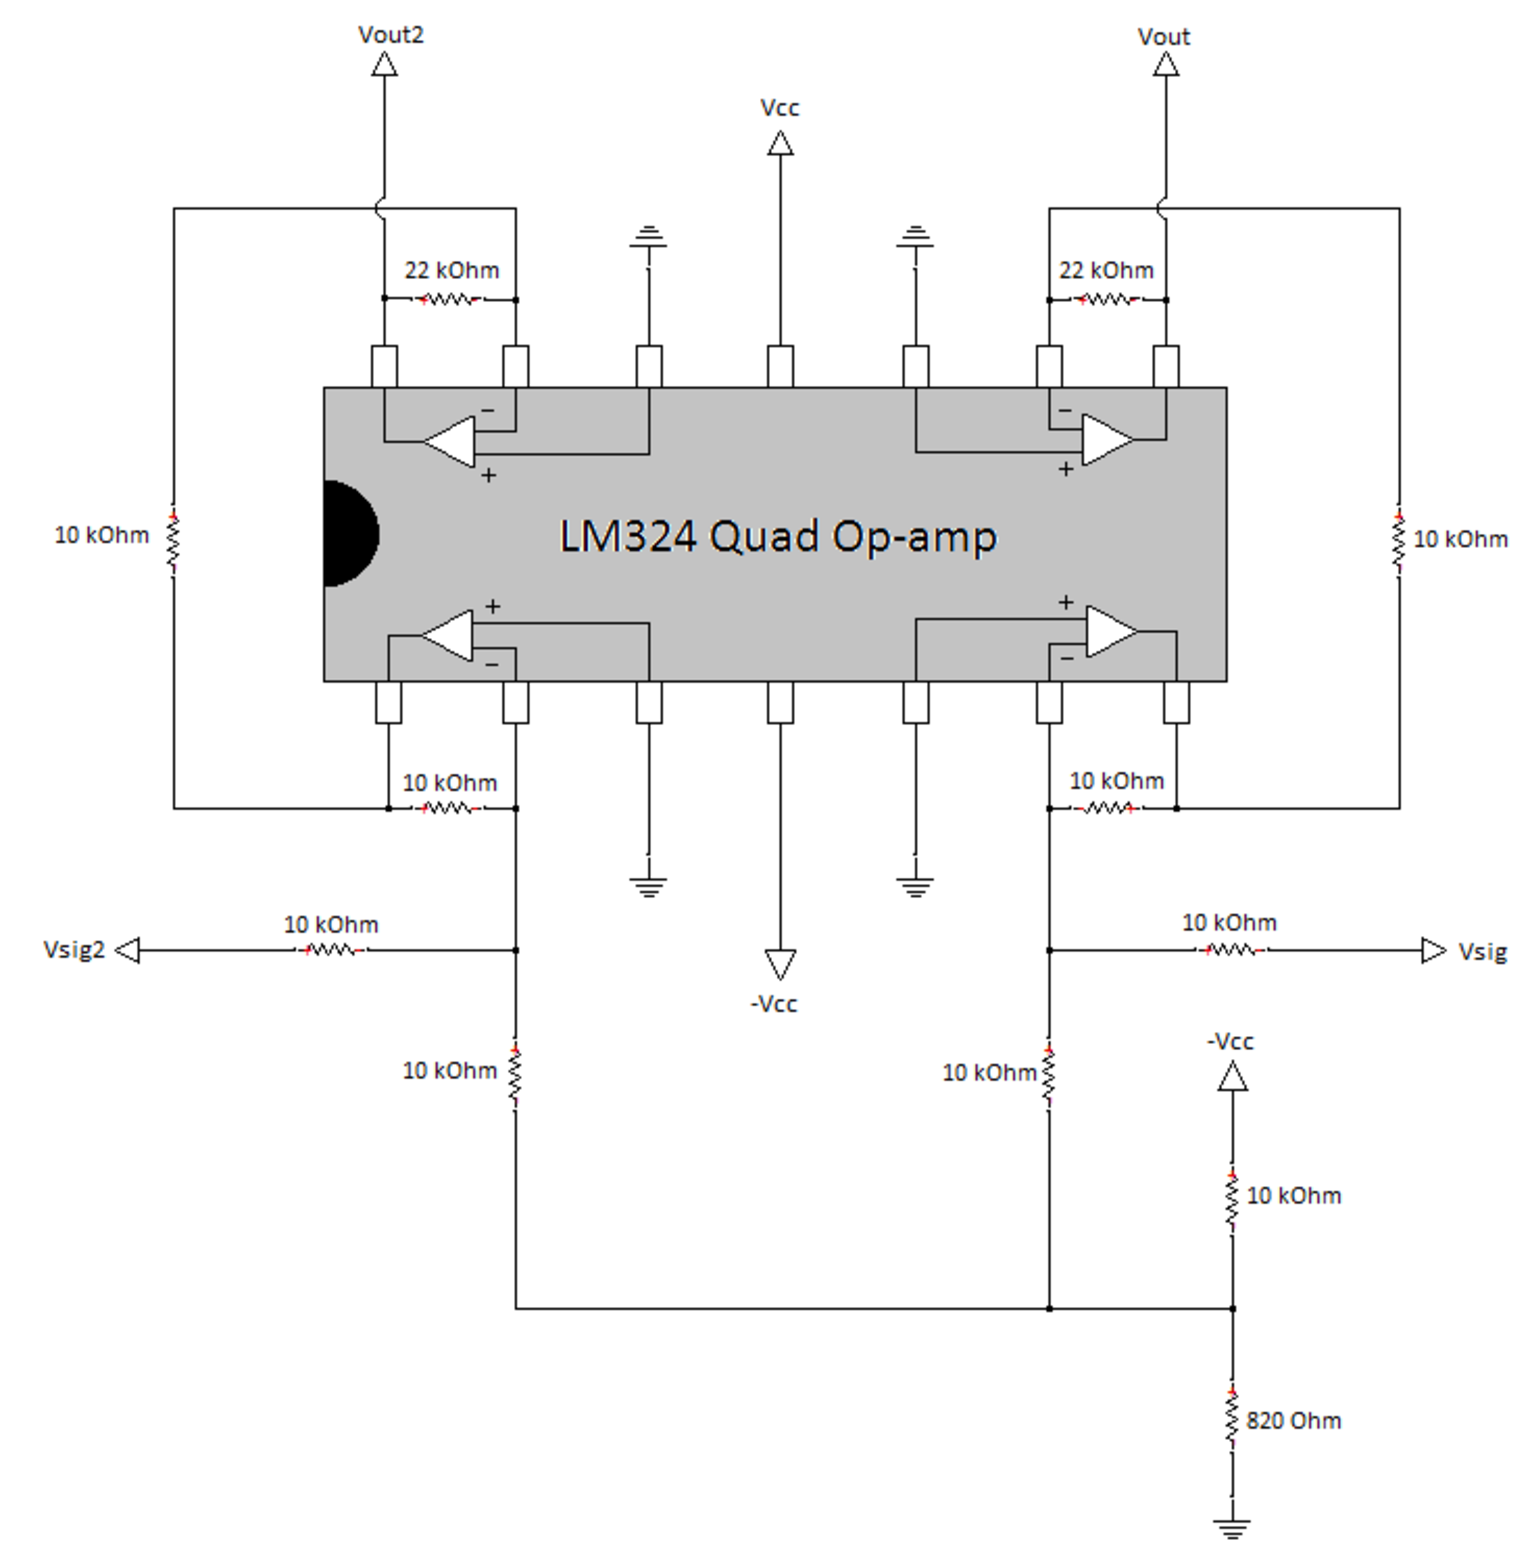
\includegraphics[width=3.5in]{LM324.pdf}
\caption{Circuit diagram for the LM324}
\label{LM324}
\end{figure}

\begin{figure}[!h]
\centering
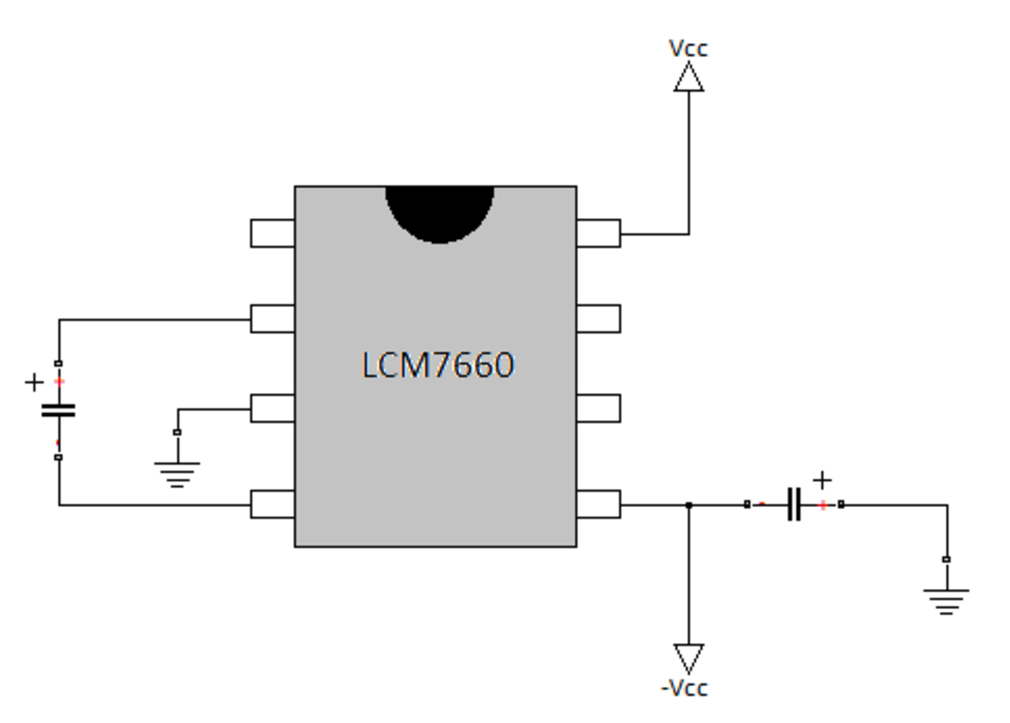
\includegraphics[width=3.5in]{LM7660.pdf}
\caption{Circuit diagram for the LM7660}
\label{LM7660}
\end{figure}

\subsection{Control}
	An electronic differential requires two separate motors being controlled by an algorithm that takes into account throttle position, turning radius, and wheel speed. The first control system flowchart was created October 2013 (Figure ~\ref{flow}). It gave the team an overall direction to plan.  First, the Arduino checks the angle reading from the steering potentiometer and determines whether the vehicle should be turning right, left, or going straight.  The angular velocity of the wheels is compared to the turning radius to determine if one of the wheels has broken contact with the ground or is slipping.
	


\begin{figure}[!h]
\centering
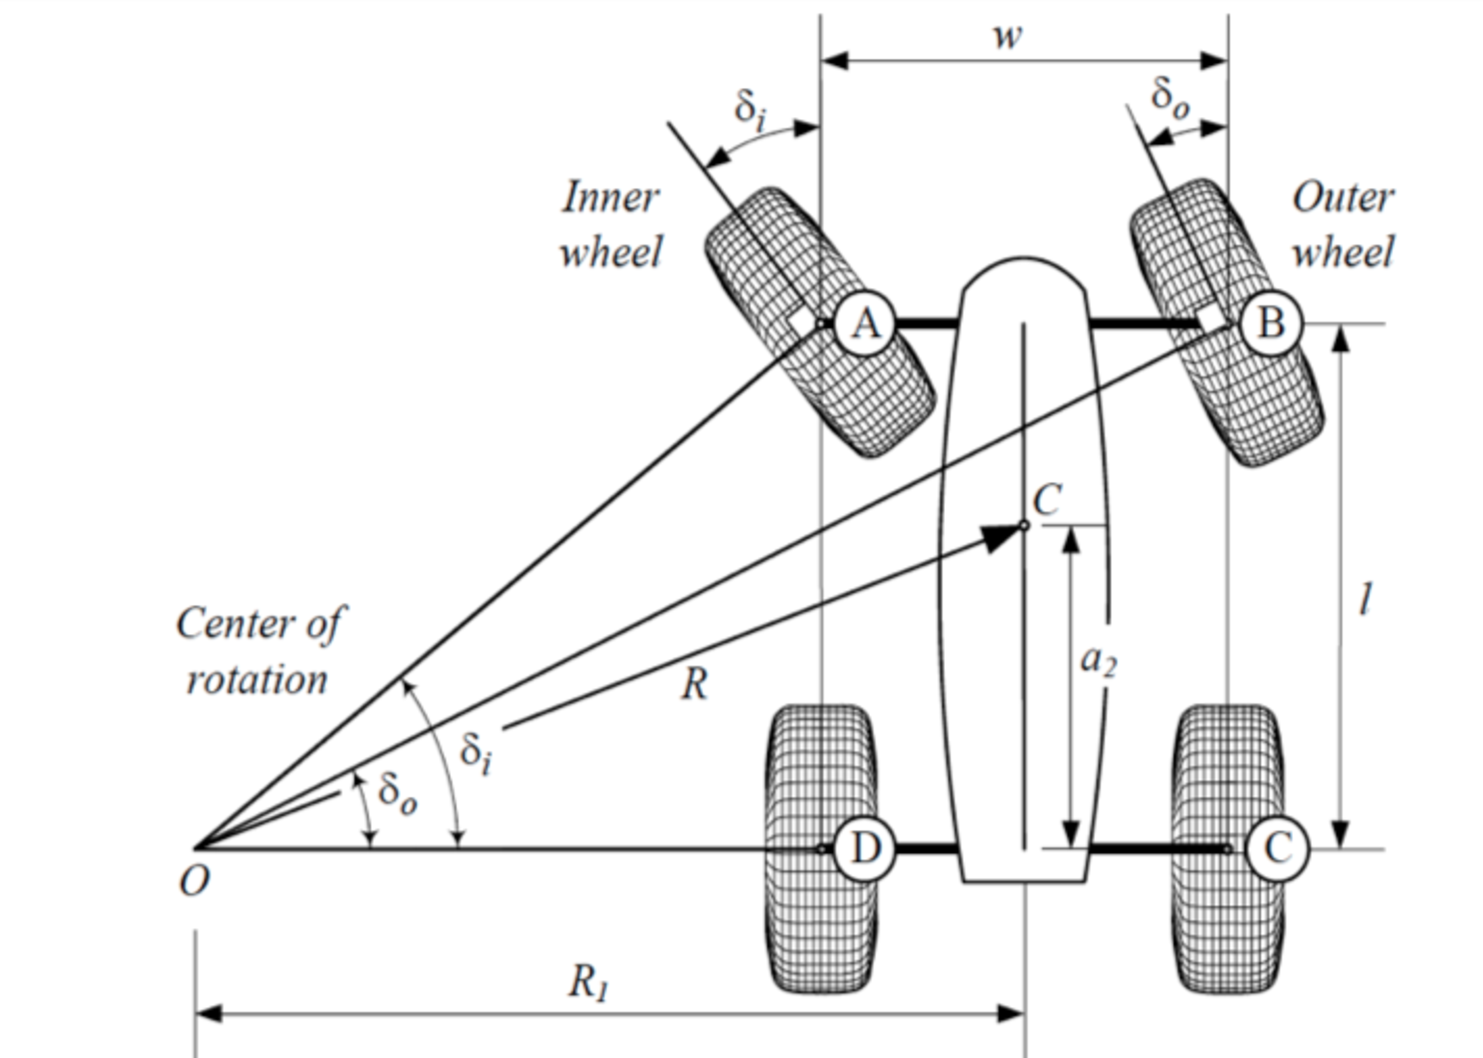
\includegraphics[width=3.5in]{ackerman.pdf}
\caption{Ackerman Steering Geometry}
\label{ackerman}
\end{figure}

	The kart's steering is in an Ackerman configuration (also referred to as Ackerman steering, Ackerman mechanism, or Ackerman geometry). Ackerman steering is a geometric arrangement of the linkages that accommodates the inner and outer wheels needing to travel tangent to circles of different radii. Figure~\ref{ackerman} is a diagram from page 387 of \emph{Vehicle Dynamics - Theory and Application} that shows Ackerman steering. 
	
	
	
	
	This configuration gives us the following equations:
	\begin{equation}
	\cot(\delta_{out}) - \cot(\delta_{in}) = \frac{w}{l}
	\end{equation}
	
	where
	$w$ is the width between the centers of the front wheels,
	$l$ is the length of the vehicle between the front and back axle, and
	$\delta_{in}$ and $\delta_{out}$ are the angles between the straight direction and the inner and outer wheel direction respectively.
	
	\begin{equation}
	R = \sqrt{a^{2} + l^{2}\cot{\delta}^{2}}
	\end{equation}
	
	\begin{equation}
	\cot{\theta} = \frac{\cot(\delta_{in}) + \cot(\delta_{out})}{2}
	\end{equation}

where
$R$ is the turning radius and
$a$ is the distance between the kart's center of gravity and the rear axle
	
	
\subsection{Sensors}

Four sensors were chosen to provide feedback to the microcontroller.  First, a potentiometer was incorporated into the accelerator pedal assembly.  The angle of the pedal is directly related to the rotation of the potentiometer shaft.  The analog voltage output from the potentiometer is directly related to the rotation of the shaft and thus was used to create an electronic throttle system.  The variable resistance changed the voltage which was then relayed to the controller and in turn, related throttle response to driver input.  

A second potentiometer was also used for detecting the steering wheel angle.  It was mounted at the end of the steering column and turned with the shaft in unison.  Using the same principles mentioned above, this device was used to provide a voltage to the controller for steering and to keep track of the rotary position of the steering shaft.  

The information concerning steering angle and throttle percent was a factor in how the controller determined which wheel required less throttle and how much overall throttle to apply.  Both the steering and throttle potentiometers were 5k� devices.  One notable difference between the steering angle potentiometer and the accelerator potentiometer was that the steering potentiometer receives its voltage from the $3.3$ Volt power out of the Arduino, rather than the $7.88$ Volts provided by the voltage regulator.  The reason for putting the steering potentiometer on the 3.3 Volt pin was to make sure the voltage didn�t fluctuate as the batteries for the kart became depleted.  The reason for powering the throttle potentiometer with the $7.88$ Volts was to increase the maximum voltage out of the potentiometer.  It was reduced due to the limitation in rotational capability caused by restricting the throttle pedal to about seventy degrees of rotation (to keep the pedal in a comfortable range of motion for the driver).  Potentiometers with resistance values above $1k\Omega$ were chosen to prevent the Arduino from getting too much current into the analog pins.  Resistance values below $15k\Omega$ were chosen in order to provide sufficient current to reduce the time needed to charge capacitors built into the Arduino�s analog input circuitry.  

Upon thoroughly researching optical encoders and affiliated mounting hardware, a pair of Koyo medium-duty optical encoders were purchased, along with mounting brackets and special couplings that minimize radial and axial loading to the encoders via their input shaft.  These encoders were mounted to the drive shafts of each motor.  They utilized 3 channels of digital signals: A, B, and Z.  Channels A and B came offset by one-half of a pulse cycle and each channel pulsed $400$ times per revolution.  Channel Z changed value once per revolution, for a pulse $\frac{1}{400}$ revolution(s) in length.  Having three channels allowed for exceptional variance in motor speed calculation.  At low speeds, the quadrature pulses on channels A and B could be used to determine rotation direction and speed and at high speeds, where direction is less important, the Z channel could be counted to get the exact number of rotations over a sample of time.  

The data sheets for these encoders can be seen in Appendix~\ref{koyo_encoders} and ~\ref{vex_encoders}.


\subsection{Software} 
\subsubsection{Overview}

To maintain consistency and keep everyone working on the same version of the code, the team formed a \emph{Github} repository. The advantage of using a repository was that everyone would have access and the ability to edit current code, as well as revert back to older versions if necessary. 

The code is divided into two main sections. 

The first section is Control Algorithm code. It contains code necessary for driving the wheels and implementing the differential control. This includes feedback processing, steering and throttle angle sensing, and calculating the proper outputs to send to the Curtis motor controllers depending on the mode (differential or solid axle).

The second section consists of data acquisition code. It is used to to test hardware and software against their design specifications. The crux of this method is to use a Secure Digital Memory (SD) card accompanied by a breakout board. It is used with the corresponding SD card library to save data into comma separated value (CSV) files.

The code described in the project can be found via the weblink provided in the ``references section''.

\subsubsection{Throttle Code}
Due to the physical location of the accelerator pedal, the available range of the throttle potentiometer is about $60\,^{\circ}$. The Arduino uses the AnalogRead function to determine the input voltage associated with the throttle position.  At the lowest position, the Arduino reads $.14$ Volts. At the highest  position, the input voltage is $4.93 V$.   Data acquisition testing showed that the voltage input to the Du\'e increases almost linearly with respect to the accelerator pedal position. This relationship can be seen in Appendix \ref{throttle}.

The range of the input voltage was programmed into the Du\'e and mapped to a $10$-bit resolution, resulting in a value between $0$ and $1023$.  If the kart is going straight or the operator selects the solid axle configuration, the same output is sent to each motor controller. In a similar way to the input mapping, the Arduino DAC output was calculated to fall between $0$ and $1023$.   

\subsubsection{Steering Code}
The steering potentiometer works in a similar way to the accelerator pedal.  It feeds a voltage to an analog input pin and is then mapped to a $10$-bit integer, which is fused to calculate the turning radius that the operator desired.  The steering potentiometer is attached to the steering column and displays about $50\,^{\circ}$ of range from hard left to hard right.  

While turning, the vehicle travels two circles of different radii simultaneously and thus with no differential action, the outer tire will drag or the inner tire will break traction with the ground. This is due to the excessive force created by traveling a smaller radius circle at the same speed as the larger circle. Taking this into consideration, the steering code needed to be as accurate as possible to increase the effectiveness of the differential simulation. As a result, this greatly reduces the force acting on the drive wheels. 

   Furthermore, because of human error and a small amount of play in the column, the steering position associated with ``straight'' fluctuates by about $15\,^{\circ}$. Because the turn radius is rather large in this range and approaches infinity at perfectly straight, the difference in output between the two motors can be minimized inside of this region.

\subsubsection{Encoder Code}
When the motors are rotating under $500$ revolutions per minute (RPM), the Arduino reads channels A and B. Channels A and B change from digital HIGH to digital LOW every time the shaft rotates $\frac{1}{400}$ of a revolution, or every $0.9\,^{\circ}$.  After one channel changes logic value, the other channel changes and the position of the encoder is recorded.  Based on the order in which this happens, the position goes up or down.  Below zero indicates counter-clockwise and above zero indicates clockwise.  After $\frac{1}{8}$ of a second, the angular velocity in RPM is calculated by the following equation:

\begin{equation}
 \omega = \frac{position\cdot fractionsOfOneSecond\cdot}{400} 
 \end{equation}
 
 One of the flaws with this code is that it takes $\frac{1}{8}$ of a second to complete. This is necessary however, as the data wouldn�t be accurate enough to be of any use if it were sped up. In order to speed up the process of computing angular velocity, a second method is used if the motors are rotating above $500$ RPM.  The Arduino ignores channels A and B and reads channel Z. The Arduino takes a timestamp and then checks channel Z to see if it is logical TRUE. Assuming it is, it then increments the value $Z_{rev}$ for $10$ total revolutions. Assuming Z has remained TRUE for $10$ revolutions, the Arduino takes a second timestamp to determine $\Delta{t} = t_{2} - t_{1}$.  Angular velocity is then computed with the following equation:
 
 \begin{equation}
 \omega =  \frac{pulseCounts}{time}
 \end{equation}
    
Encoder validation and calibration tests were performed using a stopwatch and a ramp-up function.  The Curtis controllers were fed a gradual increase in voltage to approximately $13\%$ of of the maximum.  For one minute, the wheel rotations were counted manually and the calculated angular velocity was displayed on a monitor. The total number of visible rotations was multiplied by $5$ (from the gear ratio) and compared to the calculated velocity. Velocities over $1000$ RPM are difficult to count manually, and therefore it is hard to conclude that the computed angular velocity is the actual velocity.  

\subsubsection{Differential Code}
The differential code is currently functional, however, it could still be improved upon.  To read the inputs provided by the various sensors and drive the wheels in a similar manner.  As of right now the Curtis controllers are set to Type 0 which institutes amp based Torque control.  If it detects a difference in the amperage in one of the wheels, it will compensate, which can provide a very basic form of limited slip differential control.

In order to better refine this process and provide a platform for future design teams to continue the work the 2014 senior design team has started, an algorithm has been developed that will refine the differential control, and allow for future teams to implement various extra controls (traction control, electronic stability control, 4 wheel torque vectoring, etc.).

The algorithm that is currently being employed measures the angle provided by the steering potentiometer and verifies the rate of turn that the vehicle is trying to accomplish with the wheel encoders.  Factoring out the noise by taking several samples and averaging, the code then adjusts the outputted signal, according to our control equations, and outputs a signal to allow for differential control of the motors.


\subsubsection{Data Logging}
As mentioned previously, a SD card with a breakout board was purchased to assist with testing and data acquisition. A mini-SD card fits into the slot on the breakout board. The breakout board connects to the Arduino via Serial Peripheral Interface (SPI) communication header pins. When in use, the data logging code requires the interaction of the tester via either the Arduino IDE or a pull-down switch. Typically, a tester uses the computer to enter data via the serial connection to the Arduino to specify what is being tested.

 To test the steering position, the user enters the steering position angle in degrees. The Arduino then takes ten analog input samples and saves them in a CSV file. This process is repeated as many times as specified by the user.  The user tells the Arduino to quit when they no longer want to run the test and the file is closed. For throttle position, additional data is acquired and saved to the CSV file. After the tester enters the position of the throttle pedal (in degrees), the DAC output is enabled allowing the tester to measure the voltage at the DAC output.  Then the tester enters the voltage reading and it is saved, along with the 10 samples of analog input data. 
 
The purpose of acquiring this data is threefold. The first reason was to find out how linear was the relationship between throttle position, analog input, and DAC output.  Furthermore, the saved steering position and input data could be used to compute turn radius.  Lastly, it was used to verify that the hardware was set up correctly by testing input/output before testing the system as a whole.

The data logging code was adapted to allow data acquisition of turn radius and analog steering input readings simultaneously. This process involves the user inputting the steering angle while people pushed the unpowered cart around a circle. The center of the the circled that the vehicle traveled around was marked with chalk.  Then the radius of the circle was calculated and saved to the SD card along with $25$ analog reads. Figure~\ref{steering_left} and~\ref{steering_right} show the steering input with respect to the turn radius. There are $6$ samples of left turns and $4$ samples of right turns.  It is worth noting the exponential nature of the curves.  As the vehicle has a slighter turn , the radius of curvature approaches infinity. This is evident in the increasingly upward trend as the analog input is in the middle of its range, from approximately $400$ to $600$.  In this range, the vehicle will not require a differential input to each motor.

\begin{figure}[!t]
\centering
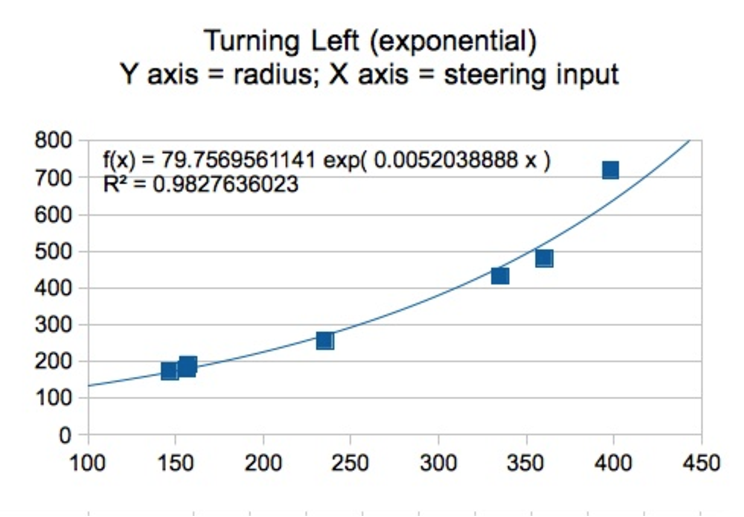
\includegraphics[width=3.5in]{steering_left.pdf}
\caption{}
\label{steering_left}
\end{figure}

\begin{figure}[!t]
\centering
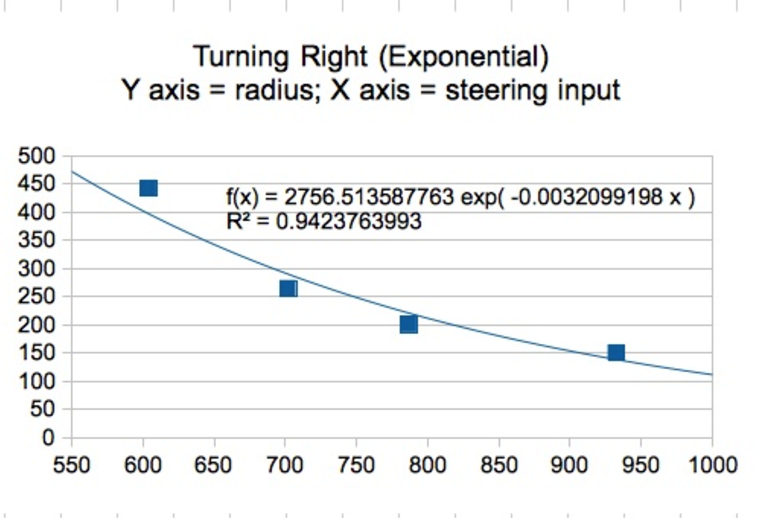
\includegraphics[width=3.5in]{steering_right.pdf}
\caption{}
\label{steering_right}
\end{figure}

\subsubsection{Curtis Parameters}

\begin{figure}[!h]
\centering
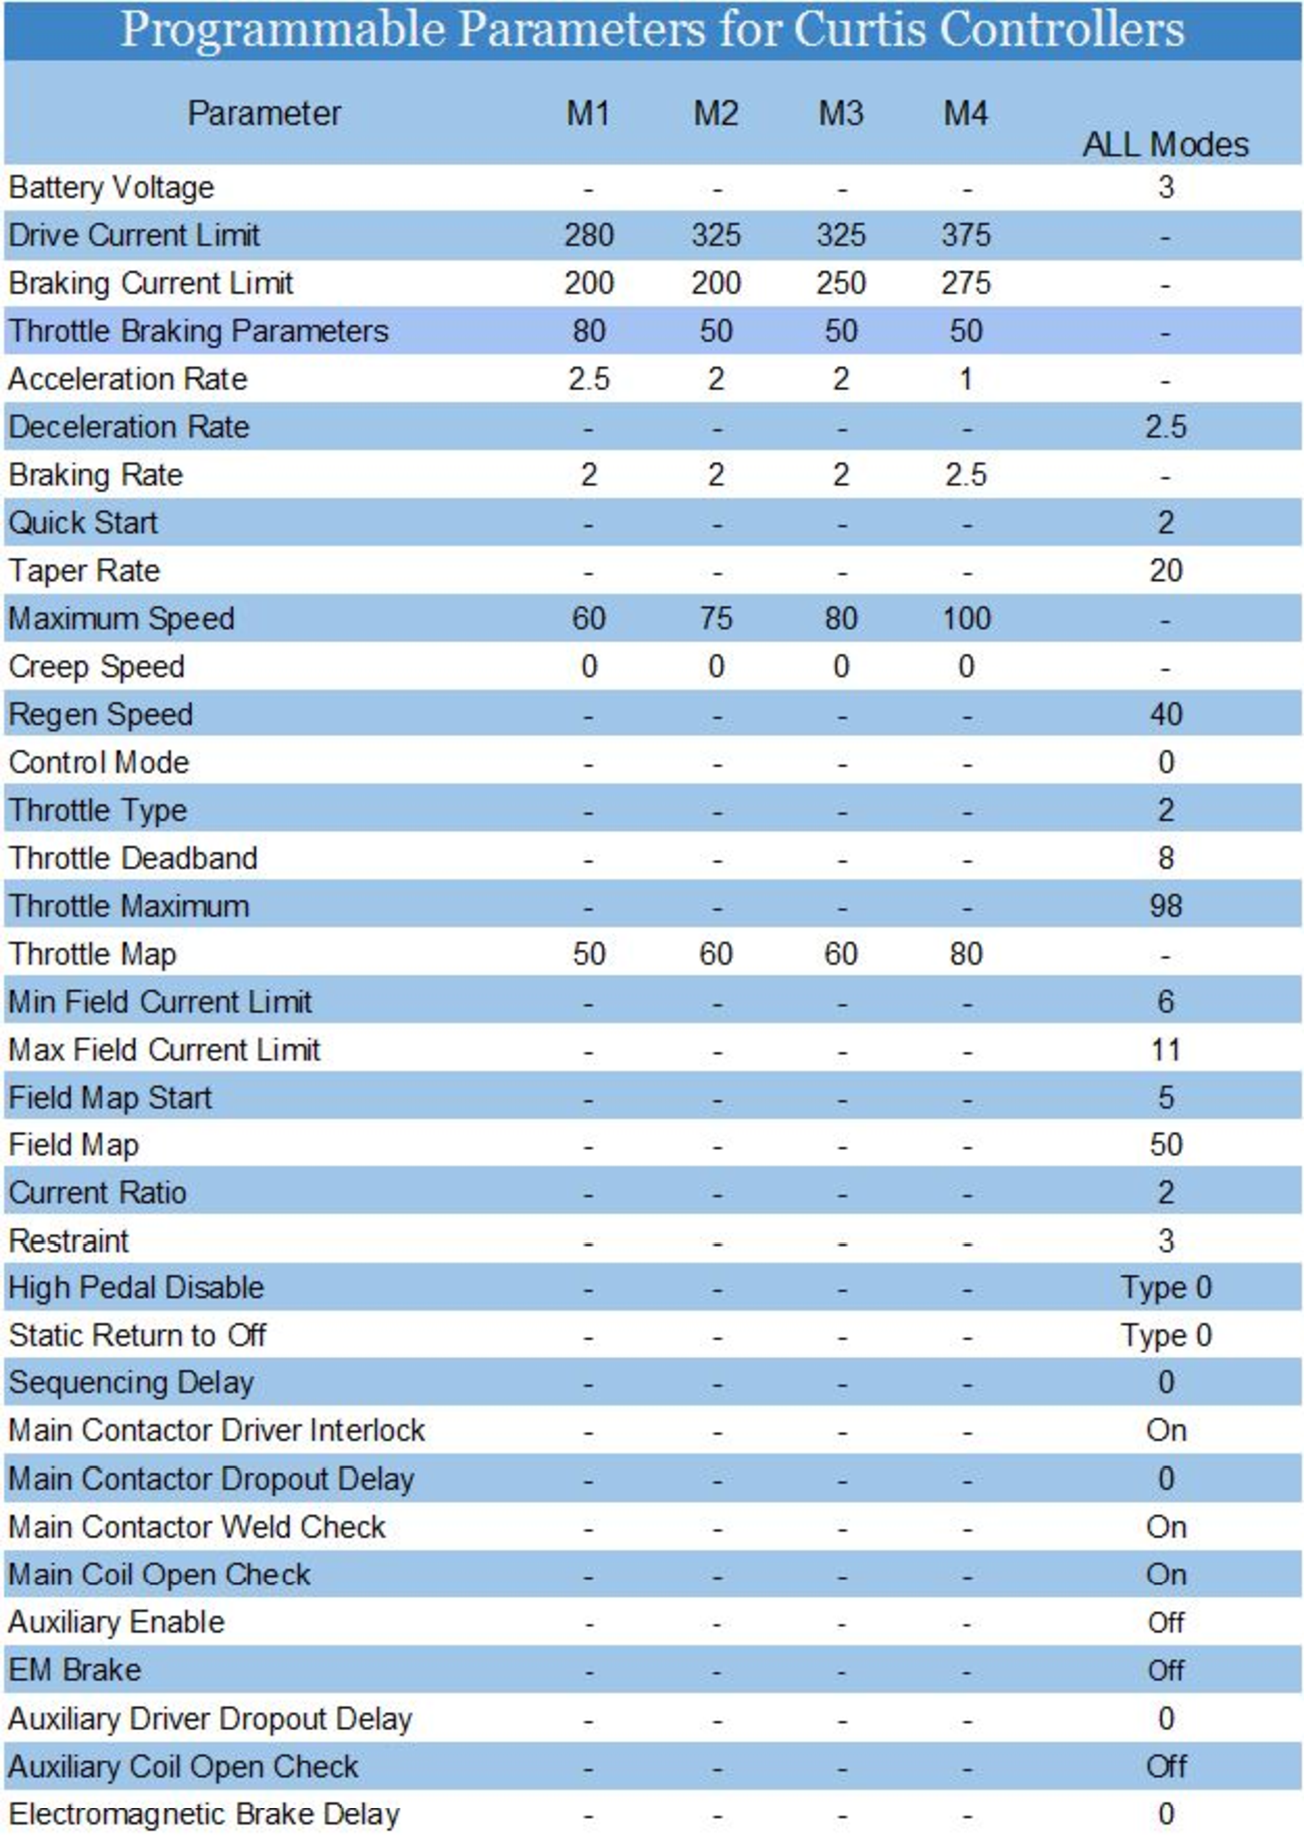
\includegraphics[width=3.5in]{curtis_param_1.pdf}
\caption*{}
\label{curtis_1}
\end{figure}

\begin{figure}[!h]
\centering
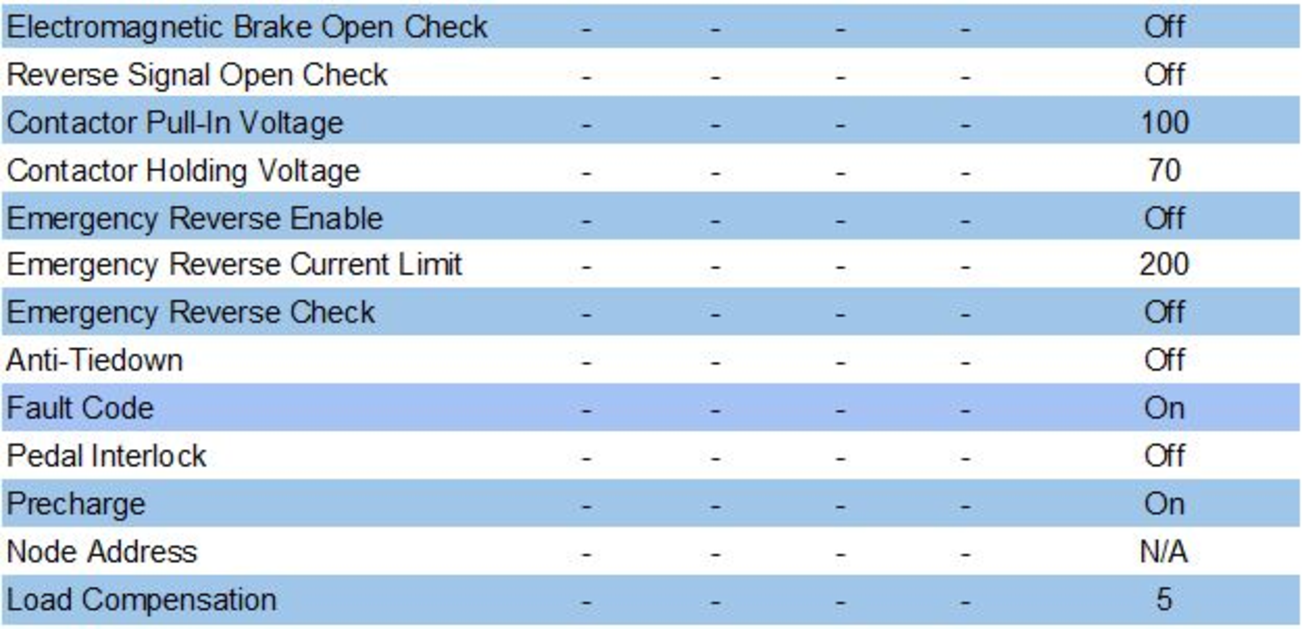
\includegraphics[width=3.5in]{curtis_param_2.pdf}
\caption{}
\label{curtis_2}
\end{figure}

%???????QUESTION????????? 

\subsection{Debugging \& Troubleshooting}
The first choice for measuring wheel speed was \emph{VEX} encoders. They were picked because they were relatively inexpensive and readily available.  These encoders, however, failed during testing because of their non-robust, plastic construction and lack of shaft bearings.  Once the motors spooled up to over $1000$ RPM, the plastic on plastic rotating parts melted due to friction and fused together, thus completely ruining the encoders.  To resolve this issue, new TRD-N(H) incremental encoders were installed that were rated to withstand both radial and axial forces of $50$ Newtons, far surpassing the ratings of the \emph{VEX} encoders.  The new encoders were also rated to 3000 continuous rpm, whereas the VEX encoders did not have a posted rpm rating because of their purpose being mainly in small robotics running low torque, low speed motors.

During the testing of the kart it was discovered that the two motors were not performing similarly.  It was noted during several tests that one motor was getting much warmer that the other and it was postulated that the warmer motor was having to work harder to compensate for some fault of the other motor.  When the underpowered motor was disassembled, it was discovered that windings inside the motor had been rubbing quite a bit, to the point that one of the wires in the field winding had been broken.  Portions of the armature windings were bent in a manner that they were outside of their specified circumference and came into contact with the field windings, thus scraping, and eventually, severing them.  To fix this, a small section of wire was pulled out of the coil and re-routed so it could be soldered back together. The armature pieces were  also repositioned to their proper positions, and all of the exposed wire was recoated with an epoxy covering.
          
Another issue that arose during the kart�s debut drive when the brakes were quick to lock up and difficult to manage. The cables were adjusted in the bracket for increased travel and a spring was added behind the pedal for improved feel. 


%////////////////////////////////////////////////////////////////////////////////////////////////////////////////////////////////////////////////////////////////////////////////////////////////////////////////////////////////////////
% TESTING
%////////////////////////////////////////////////////////////////////////////////////////////////////////////////////////////////////////////////////////////////////////////////////////////////////////////////////////////////////////

\section{Testing}
\subsection{Methods}
To quantify performance, budget-feasible tests were conducted in accordance with scaled versions of industry standard vehicular performance tests.  These tests included a simple turn radius test, a skid-pad test and a slalom test which are all are dependent on wheel and axle performance.  These are also standard performance tests for auto manufacturers and journalists.  The measure of success for these tests are shortest diameter, speed/g's, and speed/time respectively.  Out of the different tests considered, this selection displayed the greatest potential to expose the most significant differences between solid axle and controlled differential vehicle dynamics.
 

\subsection{Objectives} 
The vehicle must be tested in appropriate, documented, replicable operating conditions.  The system must show measurable improvement over a solid axle system and an forced couple (an independently driven split axle without differential control) system in the skidpad and slalom tests. 


%////////////////////////////////////////////////////////////////////////////////////////////////////////////////////////////////////////////////////////////////////////////////////////////////////////////////////////////////////////
% RESULTS
%////////////////////////////////////////////////////////////////////////////////////////////////////////////////////////////////////////////////////////////////////////////////////////////////////////////////////////////////////////
\section{Results}
When testing the kart in the solid axle configuration, it was concluded that testing could only be conducted while traveling straight. As expected, the tires skipped if the kart was turned. Testing was halted after 20 feet because the strain to the drivetrain was very large and would have resulted in damage.

Initial results have turning radii of the control system as equal to the tests of an uncoupled system.  While the results versus the solid axle system are and will remain undetermined, the control system is superior simply based on hardware considerations.



% An example of a floating figure using the graphicx package.
% Note that \label must occur AFTER (or within) \caption.
% For figures, \caption should occur after the \includegraphics.
% Note that IEEEtran v1.7 and later has special internal code that
% is designed to preserve the operation of \label within \caption
% even when the captionsoff option is in effect. However, because
% of issues like this, it may be the safest practice to put all your
% \label just after \caption rather than within \caption{}.
%
% Reminder: the "draftcls" or "draftclsnofoot", not "draft", class
% option should be used if it is desired that the figures are to be
% displayed while in draft mode.
%
%\begin{figure}[!t]
%\centering
%\includegraphics[width=2.5in]{myfigure}
% where an .eps filename suffix will be assumed under latex, 
% and a .pdf suffix will be assumed for pdflatex; or what has been declared
% via \DeclareGraphicsExtensions.
%\caption{Simulation Results.}
%\label{fig_sim}
%\end{figure}

% Note that IEEE typically puts floats only at the top, even when this
% results in a large percentage of a column being occupied by floats.
% However, the Computer Society has been known to put floats at the bottom.


% An example of a double column floating figure using two subfigures.
% (The subfig.sty package must be loaded for this to work.)
% The subfigure \label commands are set within each subfloat command,
% and the \label for the overall figure must come after \caption.
% \hfil is used as a separator to get equal spacing.
% Watch out that the combined width of all the subfigures on a 
% line do not exceed the text width or a line break will occur.
%
%\begin{figure*}[!t]
%\centering
%\subfloat[Case I]{\includegraphics[width=2.5in]{box}%
%\label{fig_first_case}}
%\hfil
%\subfloat[Case II]{\includegraphics[width=2.5in]{box}%
%\label{fig_second_case}}
%\caption{Simulation results.}
%\label{fig_sim}
%\end{figure*}
%
% Note that often IEEE papers with subfigures do not employ subfigure
% captions (using the optional argument to \subfloat[]), but instead will
% reference/describe all of them (a), (b), etc., within the main caption.


% An example of a floating table. Note that, for IEEE style tables, the 
% \caption command should come BEFORE the table. Table text will default to
% \footnotesize as IEEE normally uses this smaller font for tables.
% The \label must come after \caption as always.
%
%\begin{table}[!t]
%% increase table row spacing, adjust to taste
%\renewcommand{\arraystretch}{1.3}
% if using array.sty, it might be a good idea to tweak the value of
% \extrarowheight as needed to properly center the text within the cells
%\caption{An Example of a Table}
%\label{table_example}
%\centering
%% Some packages, such as MDW tools, offer better commands for making tables
%% than the plain LaTeX2e tabular which is used here.
%\begin{tabular}{|c||c|}
%\hline
%One & Two\\
%\hline
%Three & Four\\
%\hline
%\end{tabular}
%\end{table}


% Note that IEEE does not put floats in the very first column - or typically
% anywhere on the first page for that matter. Also, in-text middle ("here")
% positioning is not used. Most IEEE journals use top floats exclusively.
% However, Computer Society journals sometimes do use bottom floats - bear
% this in mind when choosing appropriate optional arguments for the
% figure/table environments.
% Note that, LaTeX2e, unlike IEEE journals, places footnotes above bottom
% floats. This can be corrected via the \fnbelowfloat command of the
% stfloats package.



%////////////////////////////////////////////////////////////////////////////////////////////////////////////////////////////////////////////////////////////////////////////////////////////////////////////////////////////////////////
% CONCLUSION
%////////////////////////////////////////////////////////////////////////////////////////////////////////////////////////////////////////////////////////////////////////////////////////////////////////////////////////////////////////

\section{Conclusion}
	The team solicited and received many donated parts in order to remain in the budget constraints.  These donations helped make this project possible, however they also had certain limitations and anomalies that wouldn�t have been present in new and/or higher quality equipment.  Much of the work and time was spent making many of these donated parts work as a single cohesive unit.  Some of these issues were due to frame and axle damage that could never fully be repaired (e.g. bends in the tube structure and axles).  These issues also required a reduction in the scope and goals of the project.  Traction control and regenerative braking were goals that had to be omitted as the time grew short.
	
\begin{figure}[!t]
\centering
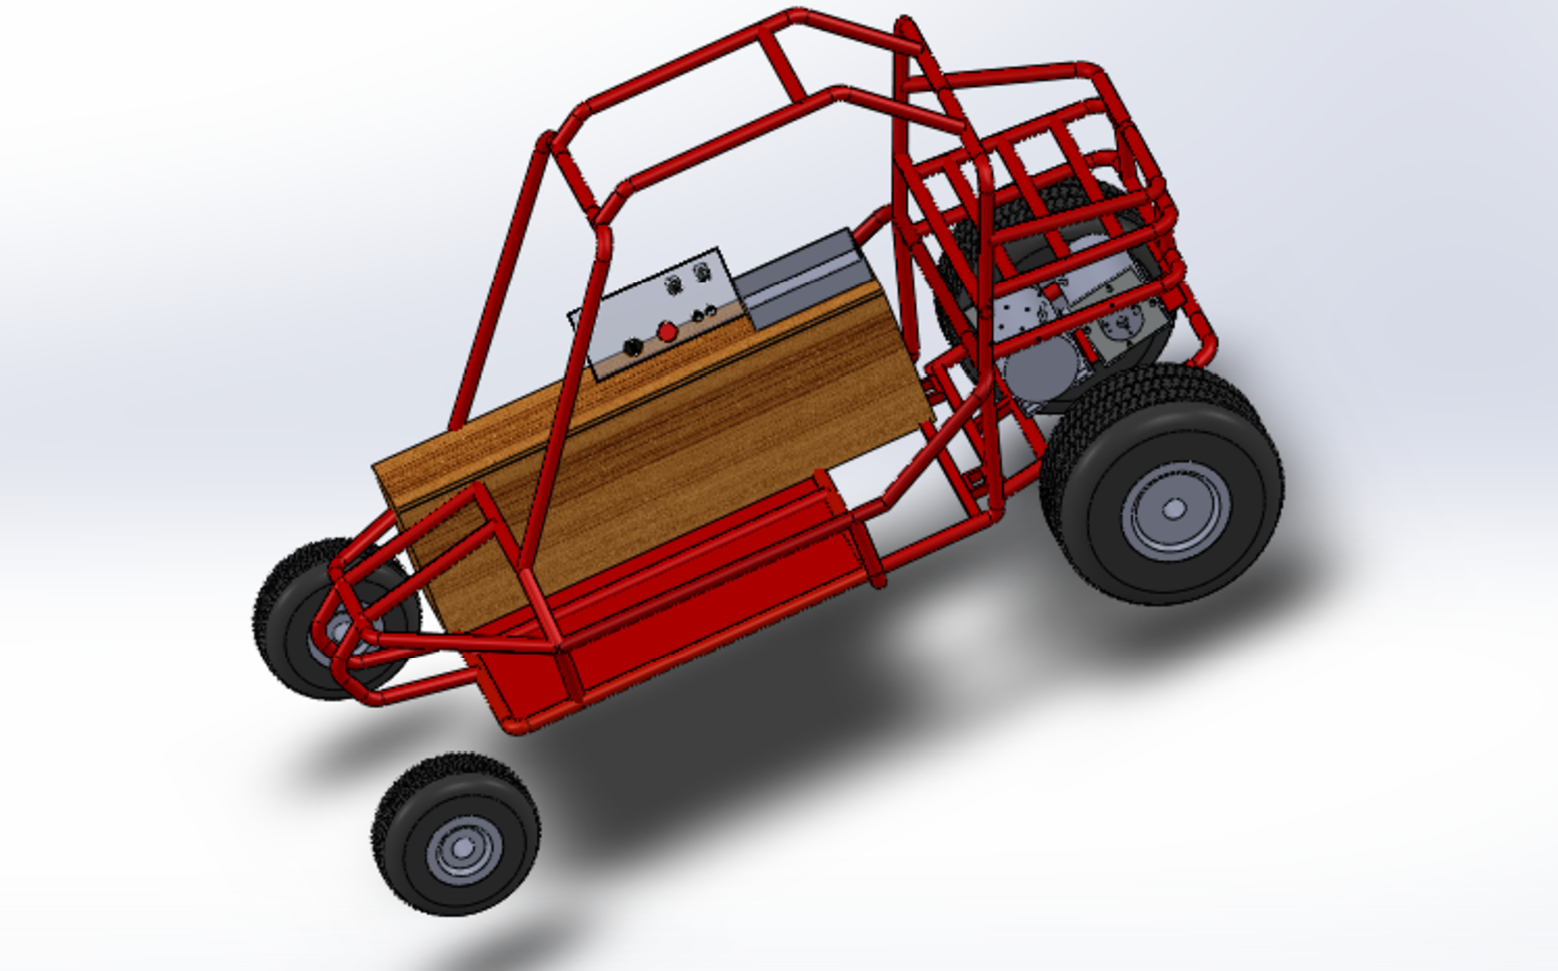
\includegraphics[width=3.5in]{final_solidwork.pdf}
\caption{Final SolidWorks Model}
\label{final_solidwork}
\end{figure}

	
Proving the advantages over the solid axle was easier than anticipated.  It was known that the physics of the situation would favor the split differential, however the severity of the kart�s reaction to the extra stress of the solid axle setup was unexpected.





%////////////////////////////////////////////////////////////////////////////////////////////////////////////////////////////////////////////////////////////////////////////////////////////////////////////////////////////////////////
%APPENDICES
%////////////////////////////////////////////////////////////////////////////////////////////////////////////////////////////////////////////////////////////////////////////////////////////////////////////////////////////////////////

% if have a single appendix:
%\appendix[Proof of the Zonklar Equations]
% or
%\appendix  % for no appendix heading
% do not use \section anymore after \appendix, only \section*
% is possibly needed

% use appendices with more than one appendix
% then use \section to start each appendix
% you must declare a \section before using any
% \subsection or using \label (\appendices by itself
% starts a section numbered zero.)
%

\ifCLASSOPTIONcaptionsoff
  \newpage
\fi
\onecolumn
\appendices

%////////////////////////////////////////////////////////////////////////////////////////////////////////////////////////////////////////////////////////////////////////////////////////////////////////////////////////////////////////
% APPENDIX A
%////////////////////////////////////////////////////////////////////////////////////////////////////////////////////////////////////////////////////////////////////////////////////////////////////////////////////////////////////////
\section{Donated Parts, Remote Kill Switch, Budget, Schedule,  }



\subsection{Donated Parts}\label{donated_parts}
The Mechatronics Senior Design group was able to procure numerous parts for the project through the generosity of various businesses and individuals.  Due to the budget constraints, these donations were necessary in order to stay within the allocated budget.  The parts donated, as well as their donors are listed below.

\begin{table}[ht] 
\caption*{{\Large Donated Parts}} % title of Table 
\centering
\resizebox{17cm}{!}{
\begin{tabular}{l l l} % centered columns (3 columns) 
\hline\hline \\%inserts double horizontal lines 
Donor & Items & Value \\ [0.5ex] % inserts table %heading 
\hline \\ % inserts single horizontal line 


%?????????QUESTION?????????? Check if these are actually  the correct values. The original table was a bit skewed.


Chris Finlayson,			&  		Motorcycle brake cables (2) 				& 		\$100 (\$50 each)\\ 
Existential Motorcycles, 		&											&		\\
Alexander, NC    			&											&		\\
						&											&		\\
Mountaintop Golf Cars      	 	&                36V Advanced Concepts EZ-GO Motors (2)  	&                \$~800(\$~400 ea.)\\
				         		&		Battery connection cables					&		\$~15\\
						&		3 hours time							&		\$~45\\
						&											&		\\
EZ-GO (Textron)              		&                Curtis Programmable Motor Controllers (3)	&		\$~1800 (\$~600 ea.)\\
				 		&		Curtis Handheld Programmer				&		\$~200\\
				  		&		Solenoids (2)							&		\$~50 (\$~25 ea.)\\
				  		&											&		\\
Joe and Ellen Reece  		&               Go-Kart chassis               	        				&                \$~400\\
				   		&											&		\\
ProMatic Automation   		&		Emergency stop button					& 		\$~50\\
				   		&		Key switch \& Interlock switch				& 		\$~75\\
				 		&		Dinrail and Other Material					& 		\$~25\\
				  		&											&		\\
Skyland Automotive  		&		12v golf cart battery						&		\$~215\\[2ex]
			         			&		 \normalsize{\textbf{Total}}				&		\$~3775\\  

				
\hline 
\end{tabular} 
}
\label{donated_parts} % is used to refer this table in the text 
\end{table}
\FloatBarrier


\subsection{Remote Kill Switch}\label{kill_switch}
Although not originally in the scope of the project, it became clear that a remote kill switch was necessary to safely operate the finished vehicle. It allows a bystander to disable the vehicle in an emergency situation if the driver of the kart is unable to do so. This process is implemented using an Arduino to communicate with the vehicle via a bluetooth connection.  The microcontroller on board intercepts the transmitted signal and shuts down the output voltage to the speed controllers.  The range of the bluetooth transmitter is one hundred meters.

	Safety algorithms mainly concern the remote kill-switch.  Other safety devices such as the dash-mounted E-stop switch and brake interlock switch do not require software to implement.   The safety switch is a device that acts as a remote kill switch in case the operator of the vehicle is unable to properly shut down the vehicle in an emergency.  This code happens first in the main loop and searches for a specific bluetooth signal.  If the signal isn't available (meaning the kill switch is left open) the loop carries on to the next task.  If the signal is received, the code immediately shuts down output voltage to the speed controllers.



\subsection{Budget}\label{budget}
\begin{table}[ht] 
\caption*{{\Large Budget}} % title of Table 
\centering
\resizebox{17cm}{!}{
\begin{tabular}{l l l} % centered columns (3 columns) 
\hline\hline \\%inserts double horizontal lines 
Vendor & Items & Cost \\ [0.5ex] % inserts table %heading 
\hline \\ % inserts single horizontal line 

VEX Robotics                &              Vex motor encoders (4)                     &                \$~52.98\\ % inserting body of the table 
BMI Karts                        &              Tie rod, brake drum, brake band   	&                \$~67.82\\
Mouser                           &               Arduino Mega 2560               	         &                \$~52.11\\
Sparkfun                        &               Bluetooth Mate Gold                   	&                \$~64.95\\
Interstate Batteries	    &		  Battery						&		\$~460.10\\
BMI Karts			   &		  Brake drum, brake band			&		\$~76.97\\
Tomtop                           &               Mini digital LCD scale             		&                \$~27.78\\
Nextwarehouse            &               Wireless bluetooth adapter      	&                \$~20.48\\
Digikey                           &               Arduino Du\'e					&                \$~59.40\\
MFG Supply                  &		   4 Hydraulic Shocks			&                \$~158.95\\
Golf Car Discounters   &               Input shaft kit                	 		&                \$~304.00\\
Sparkfun                        &               Breakout Board				&                \$~21.33\\
Mouser                           &               Micro SD Card               			&                \$~20.64\\
Tractor Supply              &                Bushings, coupler, pillow blocks    &                \$~21.84\\
Grainger			   &		   Solenoid (2)					&		\$~131.48\\
Grainger			   &		   400A fuses (2)				&		\$~26.71\\
Newark			   &    	  Voltage converter				& 		\$~13.93 \\ 
Tractor Supply		   &    	  Axle Sprocket					& 		\$~59.66 \\ 
Automation Direct	   &    	  Encoders (2)					& 		\$~270.00 \\ 
Automation Direct	   &    	  Coupling (2)					& 		\$~55.00 \\ 
Automation Direct	   &    	  Mounting bracket (2)			& 		\$~21.00 \\ 
Amazon.com		   &    	  Arduino Du\'e					& 		\$~39.70 \\ 
Sparkfun                        &               Logic Level Converter(4)		&                \$~11.73\\[2ex]
			            &		  \small{\textbf{Total}}		&		\$~2138.60 \\  
\hline 
\end{tabular} 
}
\label{budget_parts} % is used to refer this table in the text 
\end{table}



\subsection{Schedule}\label{schedule}
To budget for the limited time, the team implemented a Gantt Chart to keep track of the progress of the project.  The Gantt Chart provided an effective means to forecast potential bottlenecks in the design.  This allowed the team to compensate and adjust for these problems in order to maintain the necessary pace to complete the project. 

Below are two Gantt charts that illustrate our anticipated timeline and the project�s actual timeline. One of the biggest deviation between the two was due to vehicle repair and part replacement. The section of our timeline was stretched because of part procurement for our modified chassis (this includes significant vehicular weight and increased drive power) and part fitting (items needing to be fabricated or modified).

\begin{figure}[!htb]
\centering
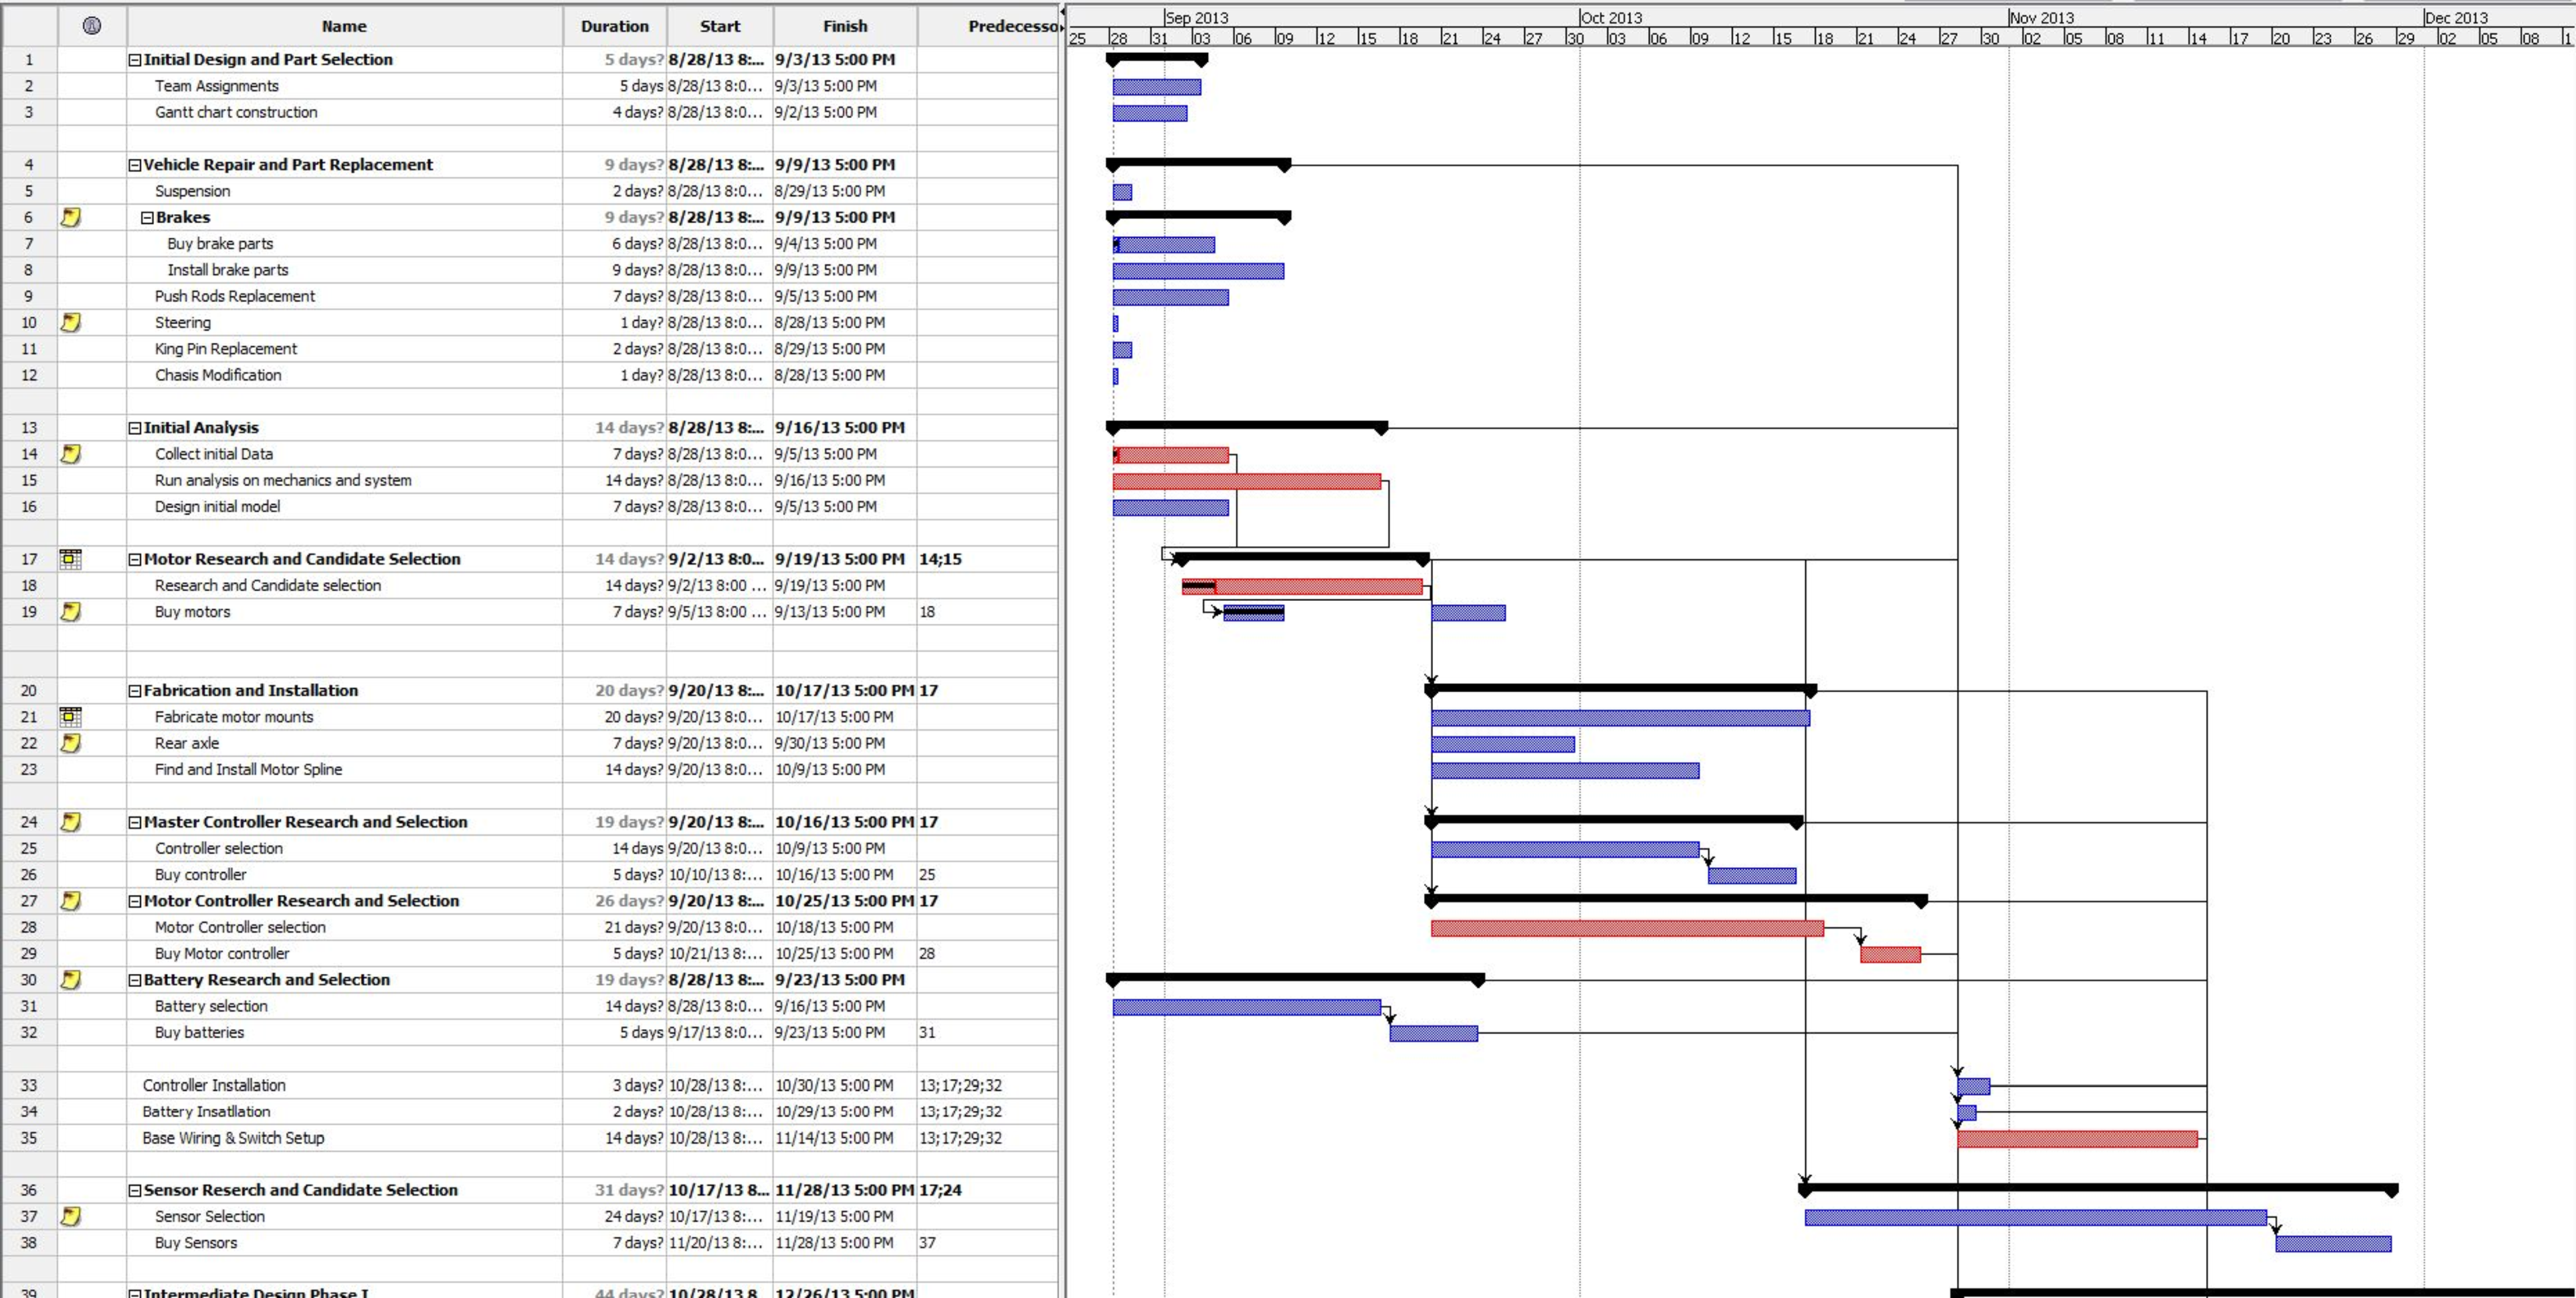
\includegraphics[width=1\textwidth]{anticipated_schedule.pdf}
\caption*{Anticipated Schedule}
\label{anticipated_schedule}
\end{figure}
\FloatBarrier

\begin{figure}[!htb]
\centering
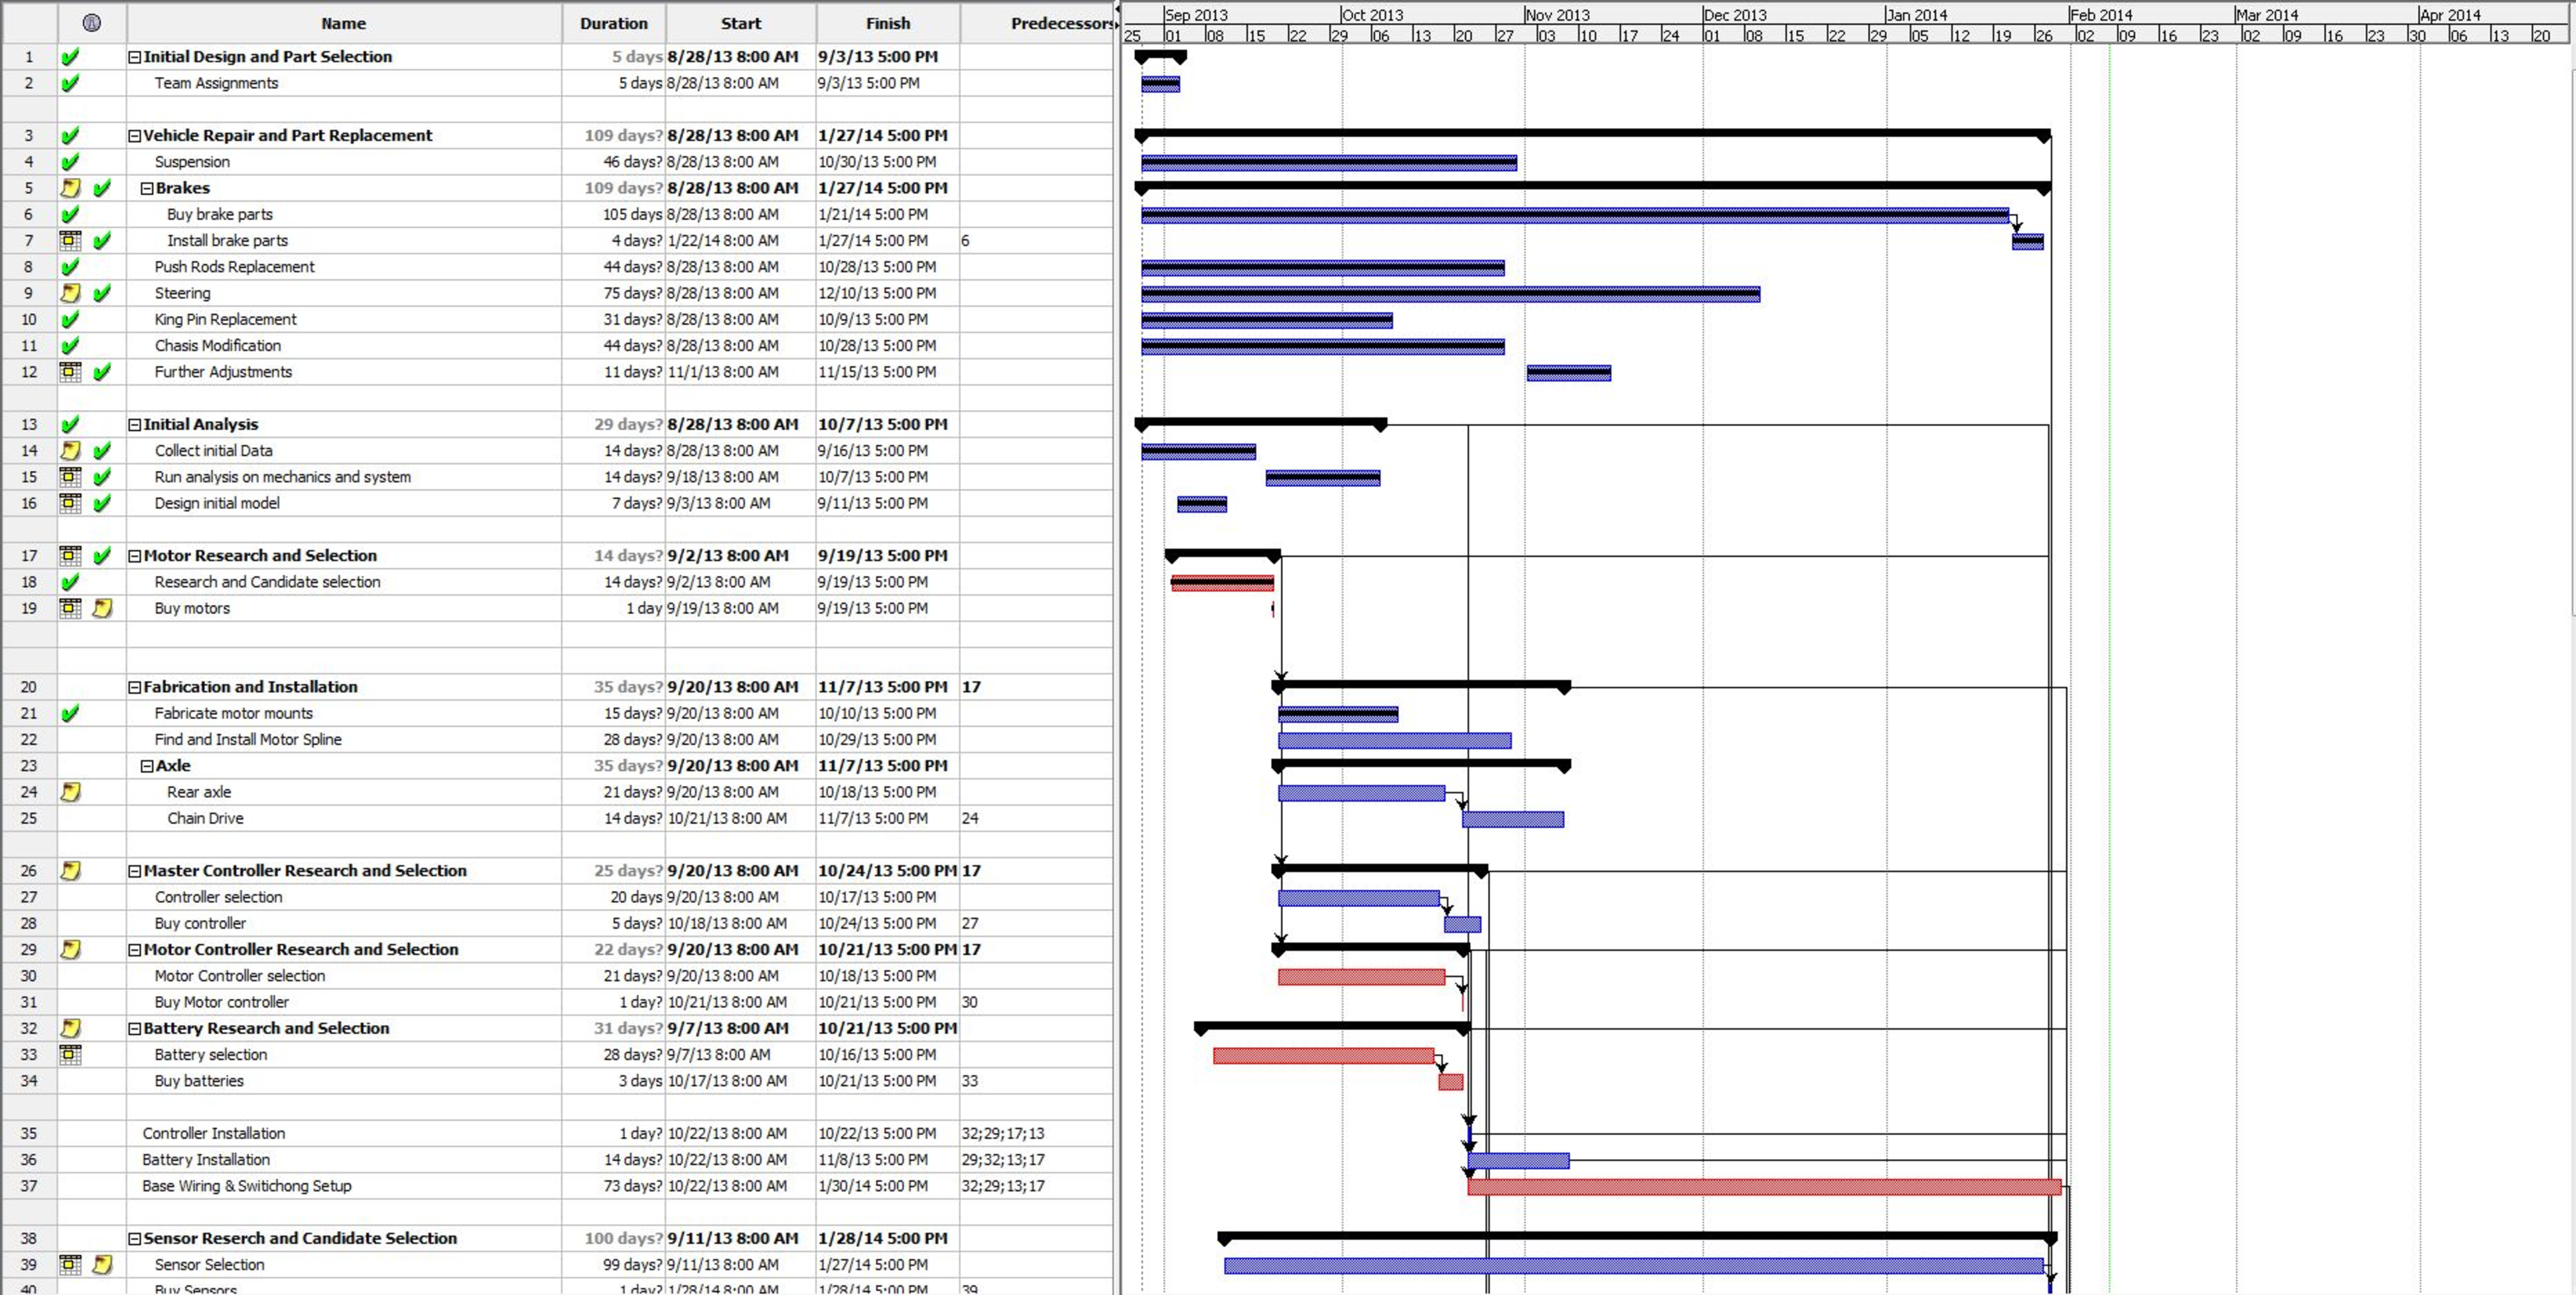
\includegraphics[width=1\textwidth]{actual_schedule.pdf}
\caption*{Actual Schedule}
\label{actual_schedule}
\end{figure}
\FloatBarrier

\newpage
\subsection{Traction Control}
When designing the traction control, the flow chart in Figure~\ref{flow} helped in overall direction in the planning phase. In the diamond decision blocks above, $\omega$ represents wheel speed and $\theta$ represents steering angle. Through the combination of tests points, the control scheme falls to one of $5$ cases. Once the ``state'' of the vehicle has been determined, the controller will calculate the necessary adjustments in power to return the kart to a non-slipping state. As the project moved forward, this control scheme became obsolete.
\begin{figure}[!b]
\centering
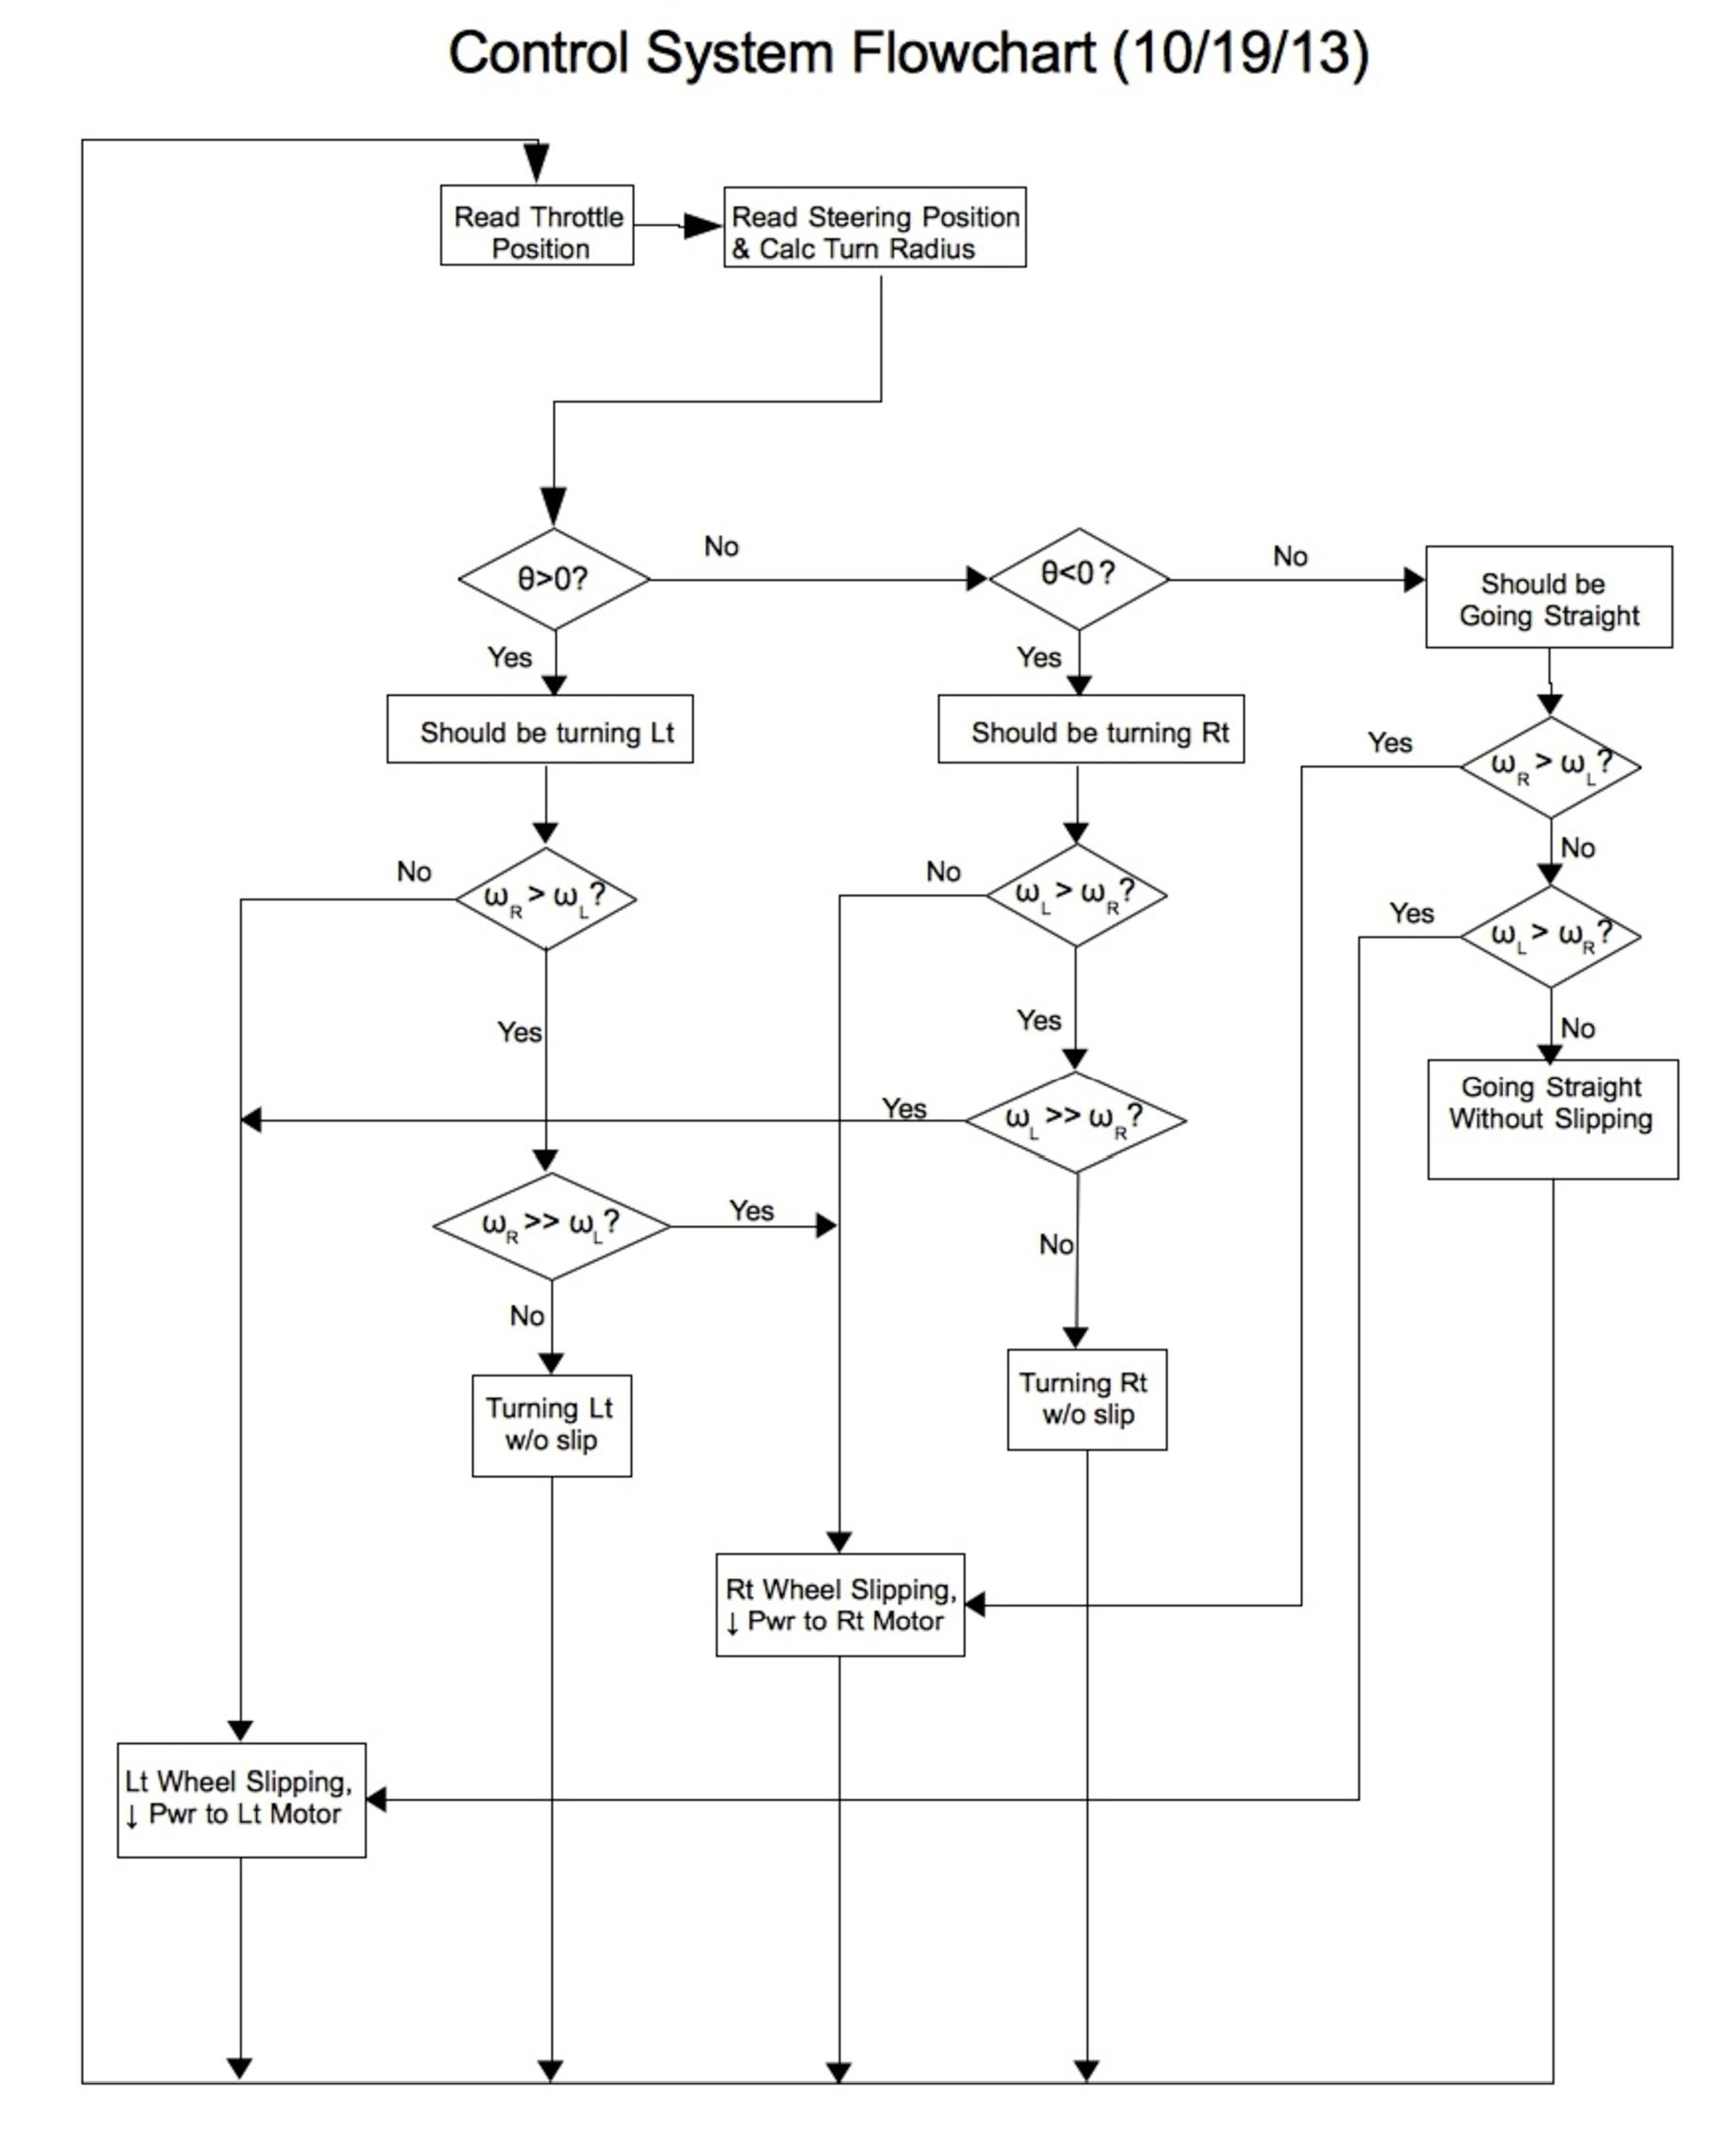
\includegraphics[width=.8\textwidth]{flowchart.pdf}
\caption{Control Flow Chart}
\label{flow}
\end{figure}
\FloatBarrier

	


%////////////////////////////////////////////////////////////////////////////////////////////////////////////////////////////////////////////////////////////////////////////////////////////////////////////////////////////////////////
% APPENDIX B
%////////////////////////////////////////////////////////////////////////////////////////////////////////////////////////////////////////////////////////////////////////////////////////////////////////////////////////////////////////
\newpage
\section{Data Tables and Graphs}
This test reflects the rolling resistance of the kart before any actual components were added.  Three people were riding the cart to simulate the additional weight of said components.  The distance was $40$ feet, enough to reach a steady state.

\subsection{Initial Horse Power Calculation}\label{initial_horse}
\begin{figure}[h!]
\centering
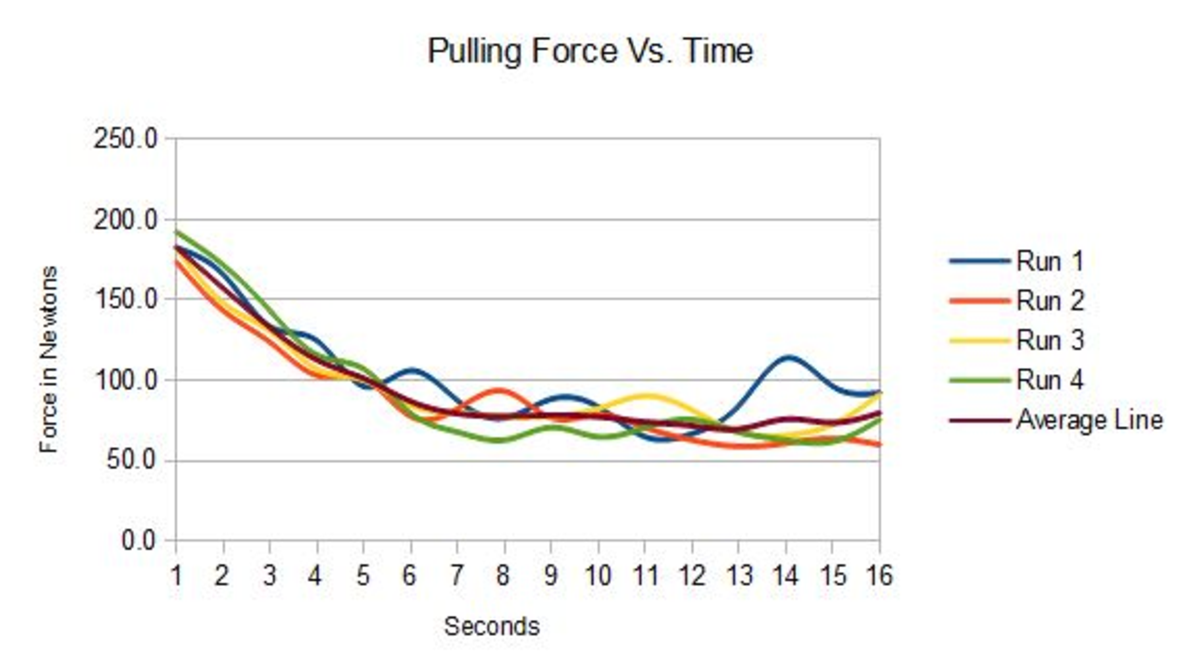
\includegraphics[width=1\textwidth]{appendix_b1.pdf}
\caption*{}
\label{pulling_force}
\end{figure} 
\FloatBarrier

% you can choose not to have a title for an appendix
% if you want by leaving the argument blank
\newpage
\subsection{Power Requirements for Rolling Resistance} \label{power_req}                       %??????QUESTION??????
\begin{figure}[h!]
\centering
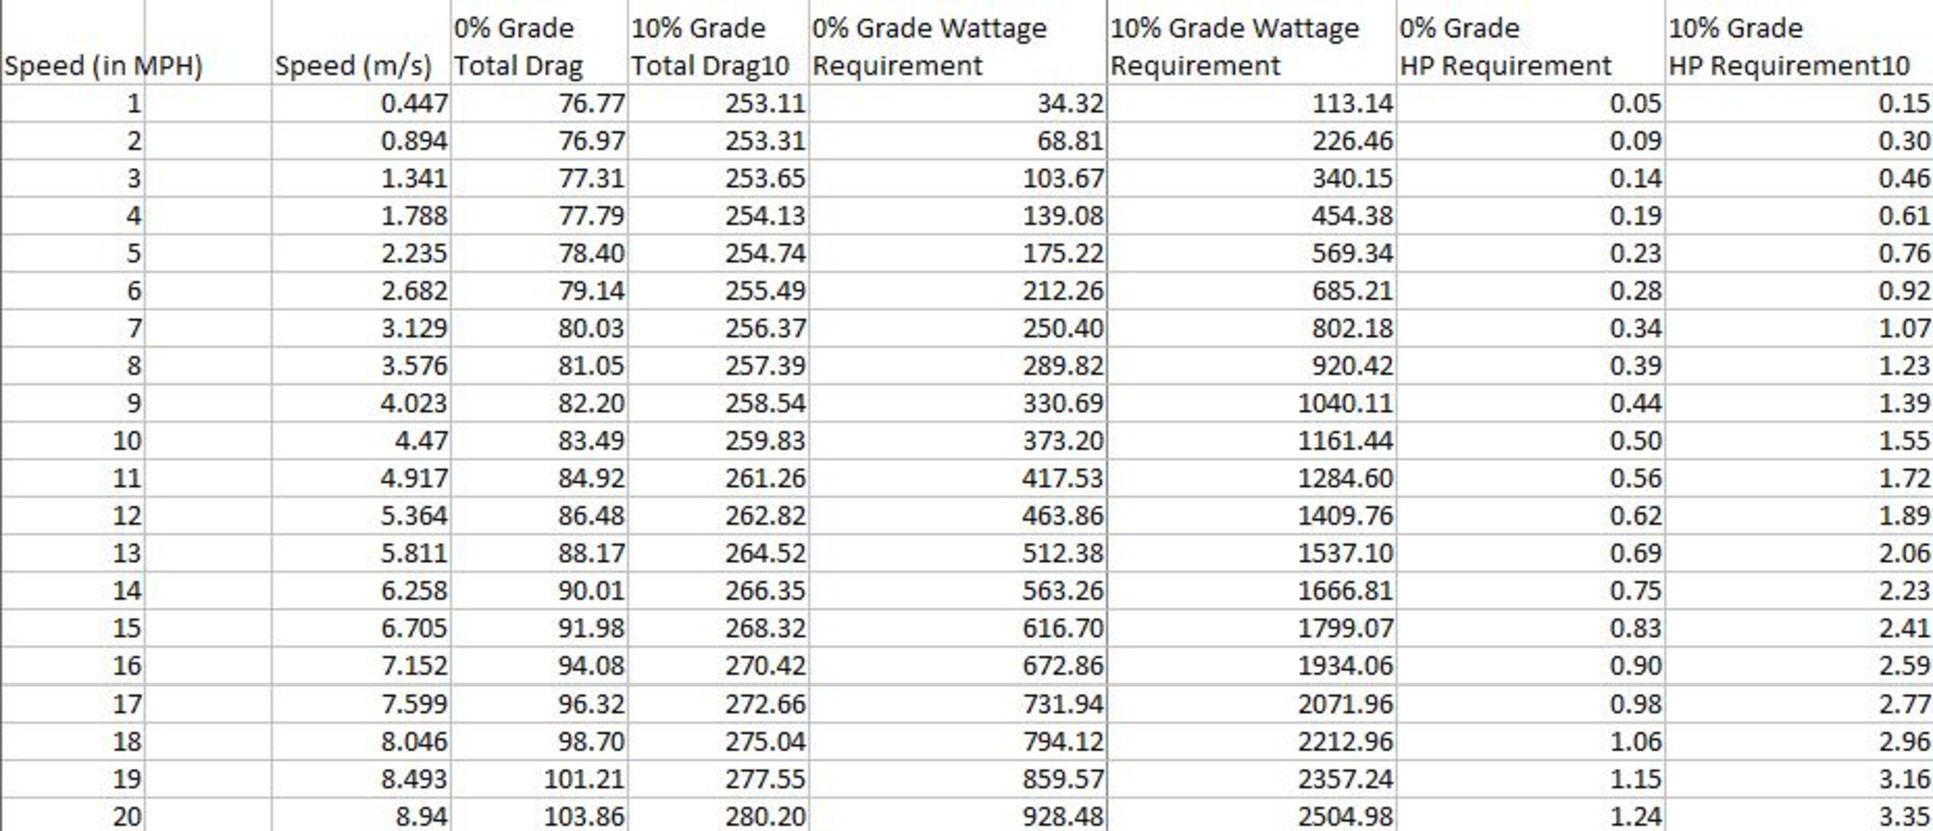
\includegraphics[width=1\textwidth]{rolling_resistance.pdf}
\caption*{}
\label{rolling_resistance}
\end{figure} 
\FloatBarrier

\subsection{Throttle Response Graph}\label{throttle}
 In order to determine if the accelerator input was linear and verify the output voltage going to the Curtis speed controllers, an SD card was purchased and code written to acquire data including accelerator position, input to the Arduino, and measured output voltage to the controllers.  The information was saved to the SD card and converted to a spreadsheet.  The graph below indicates the response is close to linear.

\begin{figure}[!htb]
\centering
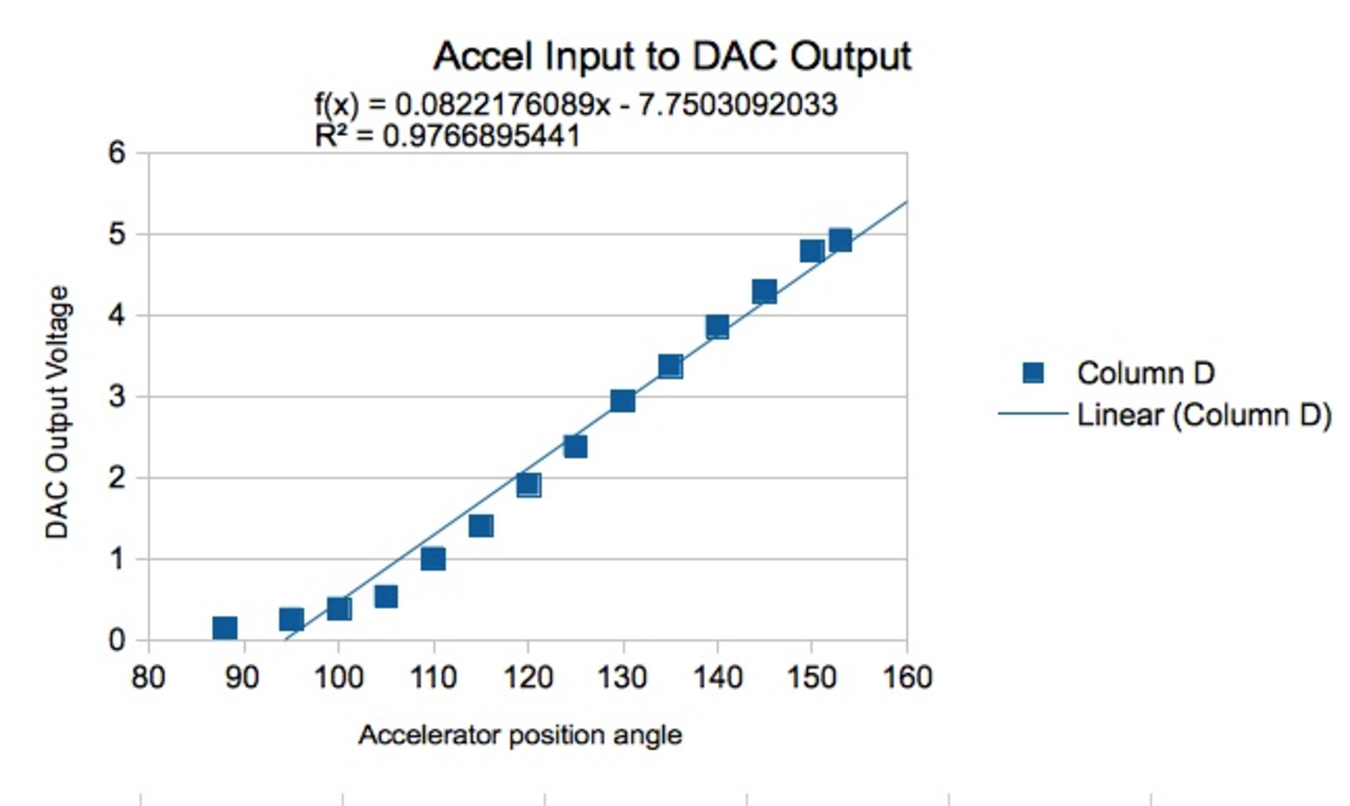
\includegraphics[width=.87\textwidth]{accel_input_data.pdf}
\caption*{}
\label{accel_inout_data}
\end{figure}

\begin{figure}[!htb]
\centering
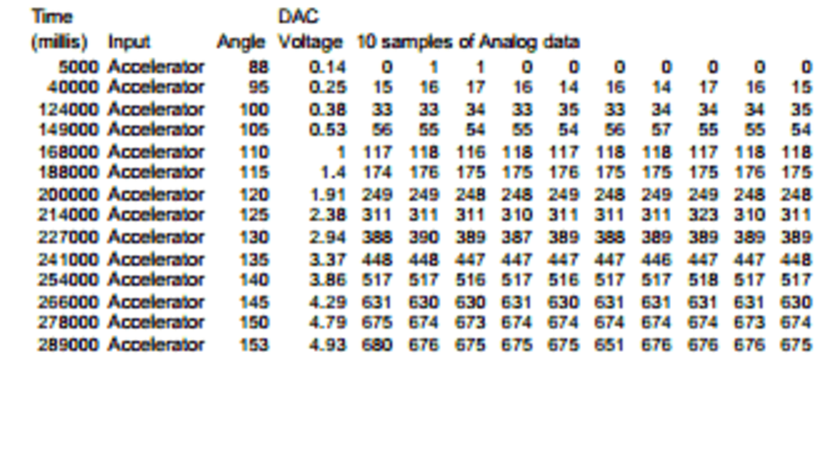
\includegraphics[width=.87\textwidth]{accel_data_chart.pdf}
\caption*{}
\label{accel_data_chart}
\end{figure}

\newpage
\subsection{Center of Mass Calculations}\label{B4}
\begin{figure}[!htb]
\centering
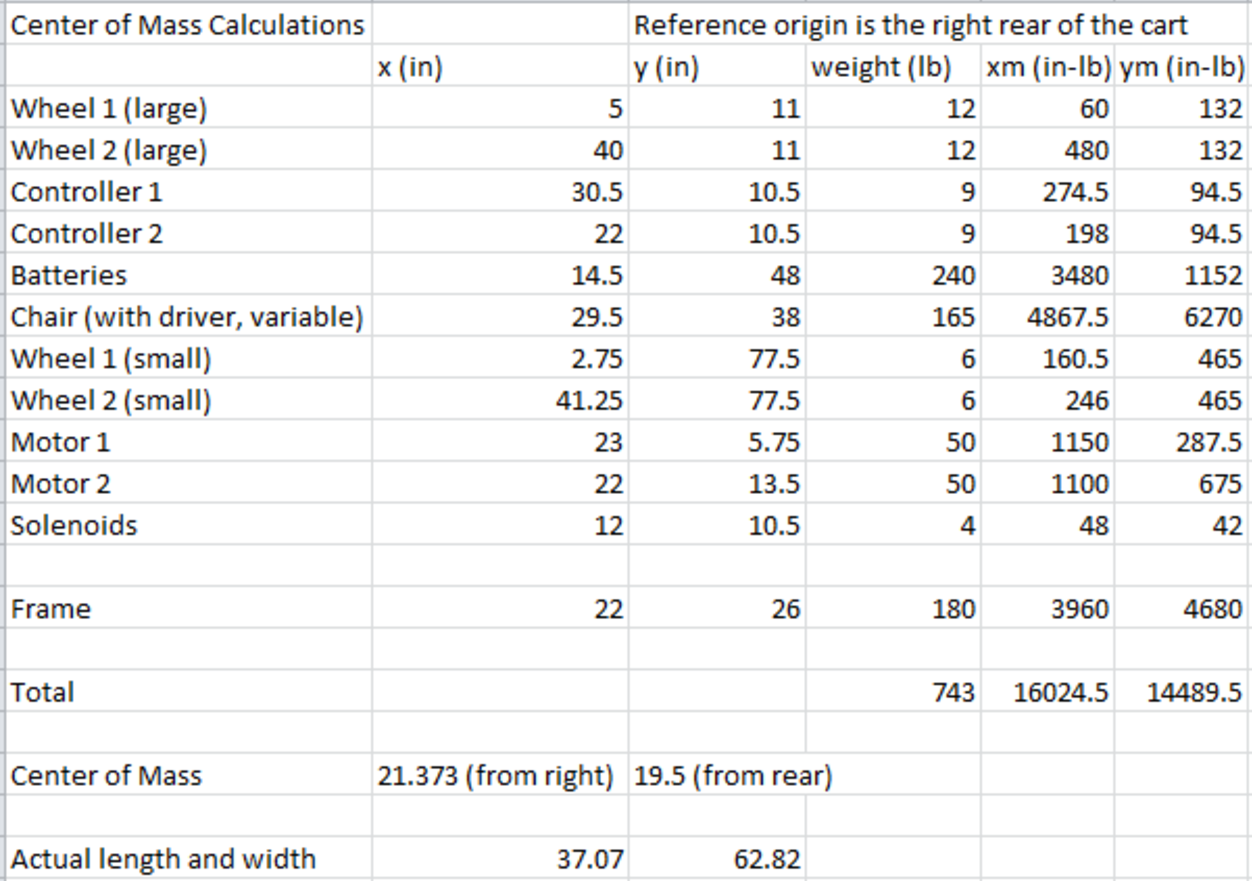
\includegraphics[width=1\textwidth]{center_of_mass.pdf}
\caption*{}
\label{centerofmass}
\end{figure}





%////////////////////////////////////////////////////////////////////////////////////////////////////////////////////////////////////////////////////////////////////////////////////////////////////////////////////////////////////////
% APPENDIX C
%////////////////////////////////////////////////////////////////////////////////////////////////////////////////////////////////////////////////////////////////////////////////////////////////////////////////////////////////////////
\newpage
\section{Data Sheets}
\subsection{Advanced D.C. Motors AY4-4001 Motors}\label{motor_torque}
\begin{figure}[!htb]
\centering
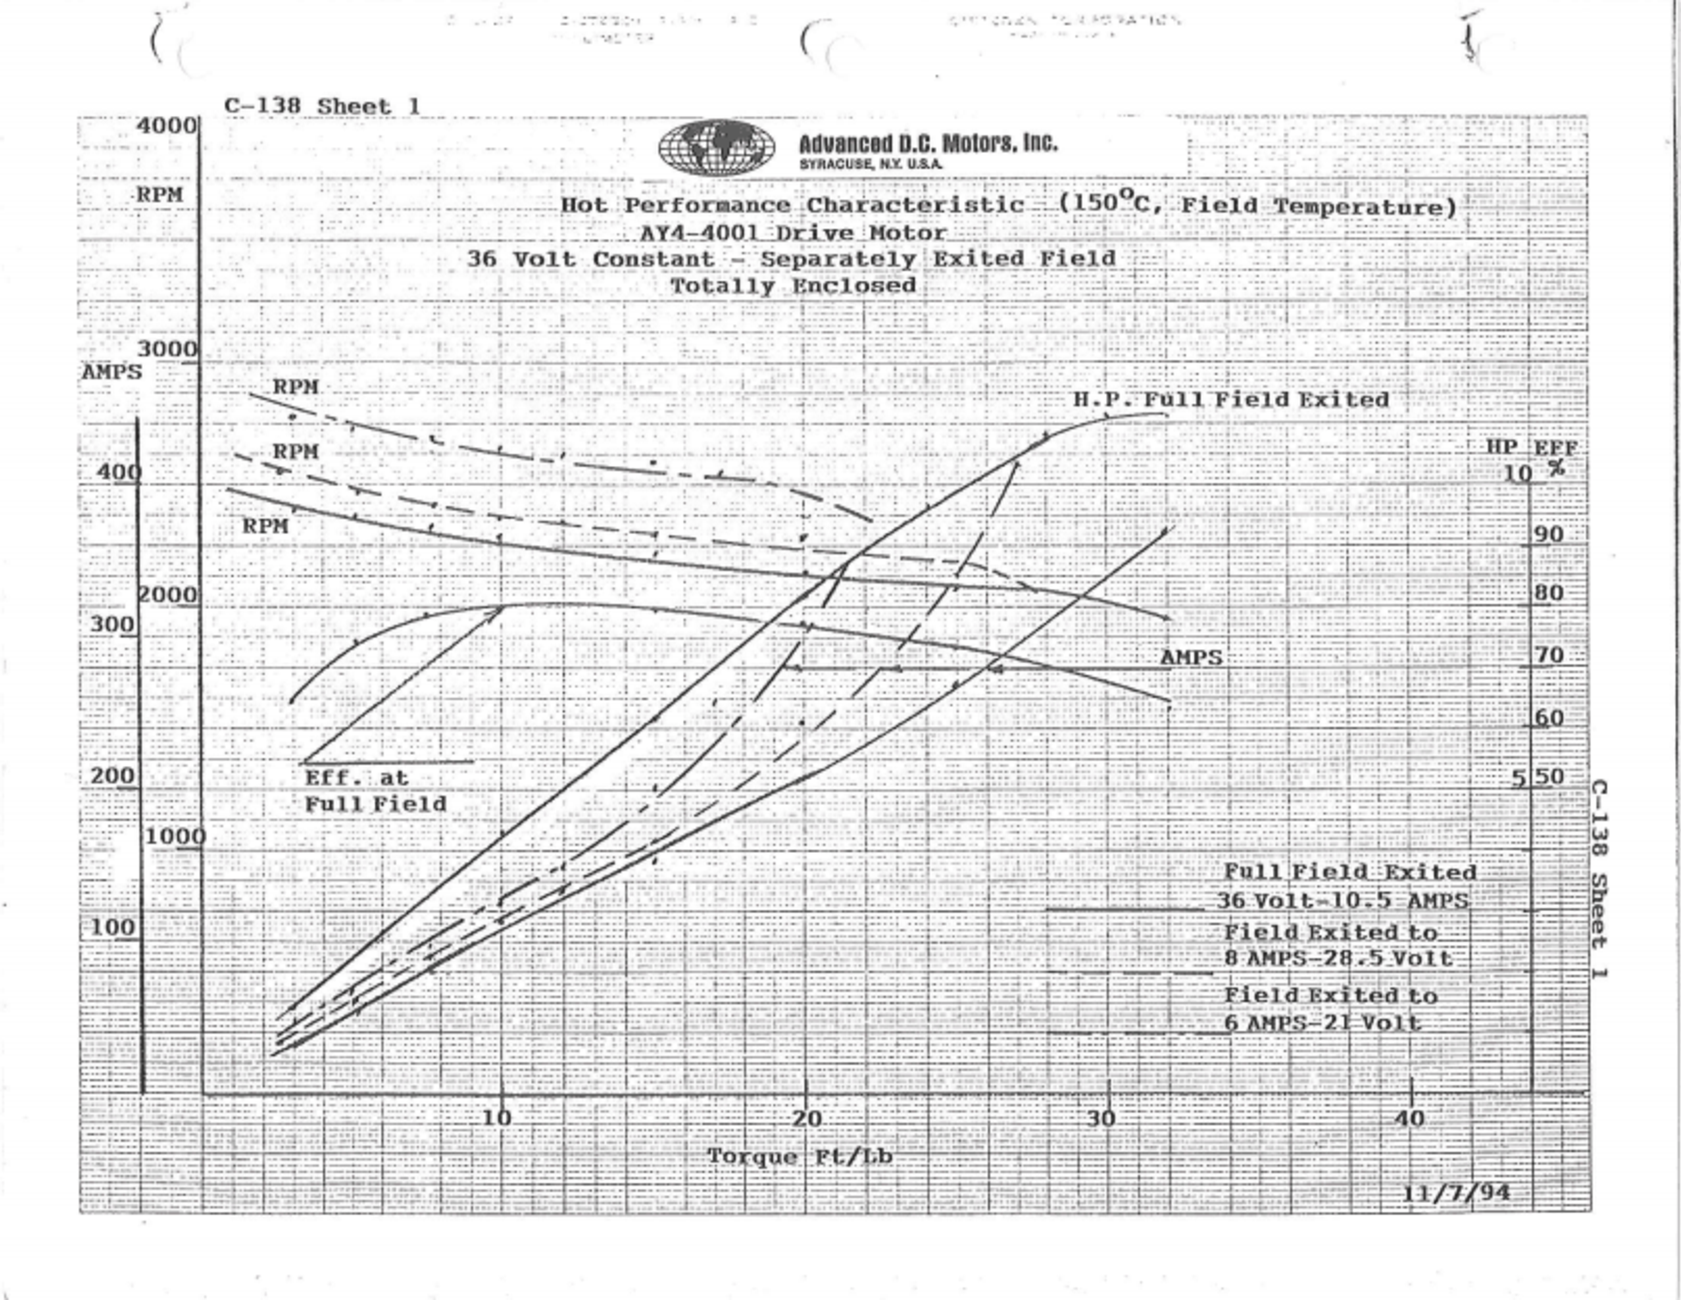
\includegraphics[width=1\textwidth]{torque_curve.pdf}
\caption*{}
\label{torquecurve}
\end{figure}
\FloatBarrier

\newpage
\subsection{Arduino Pin Layout }\label{arduino_pin}
\begin{figure}[!htb]
\centering
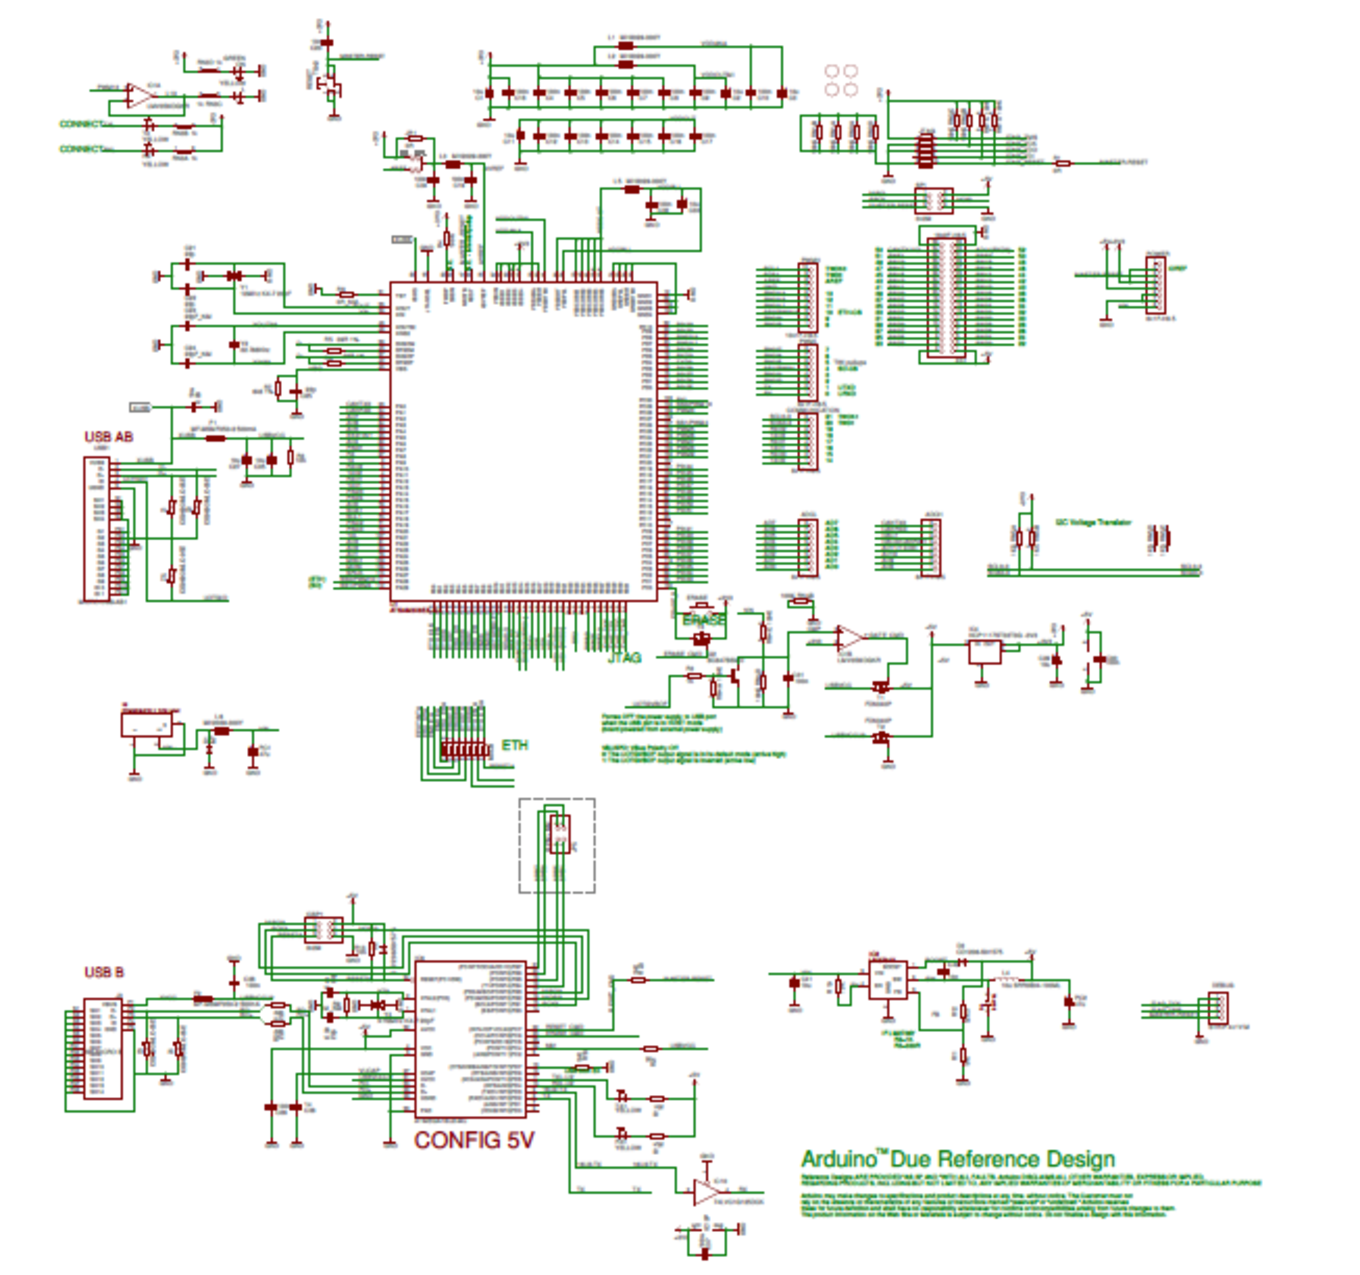
\includegraphics[width=1\textwidth]{arduino_pinout.pdf}
\caption*{}
\label{arduino_pinout}
\end{figure}
\FloatBarrier

\newpage
\subsection{Broken Field Windings}\label{broken_windings}
\begin{figure}[!htb]
\centering
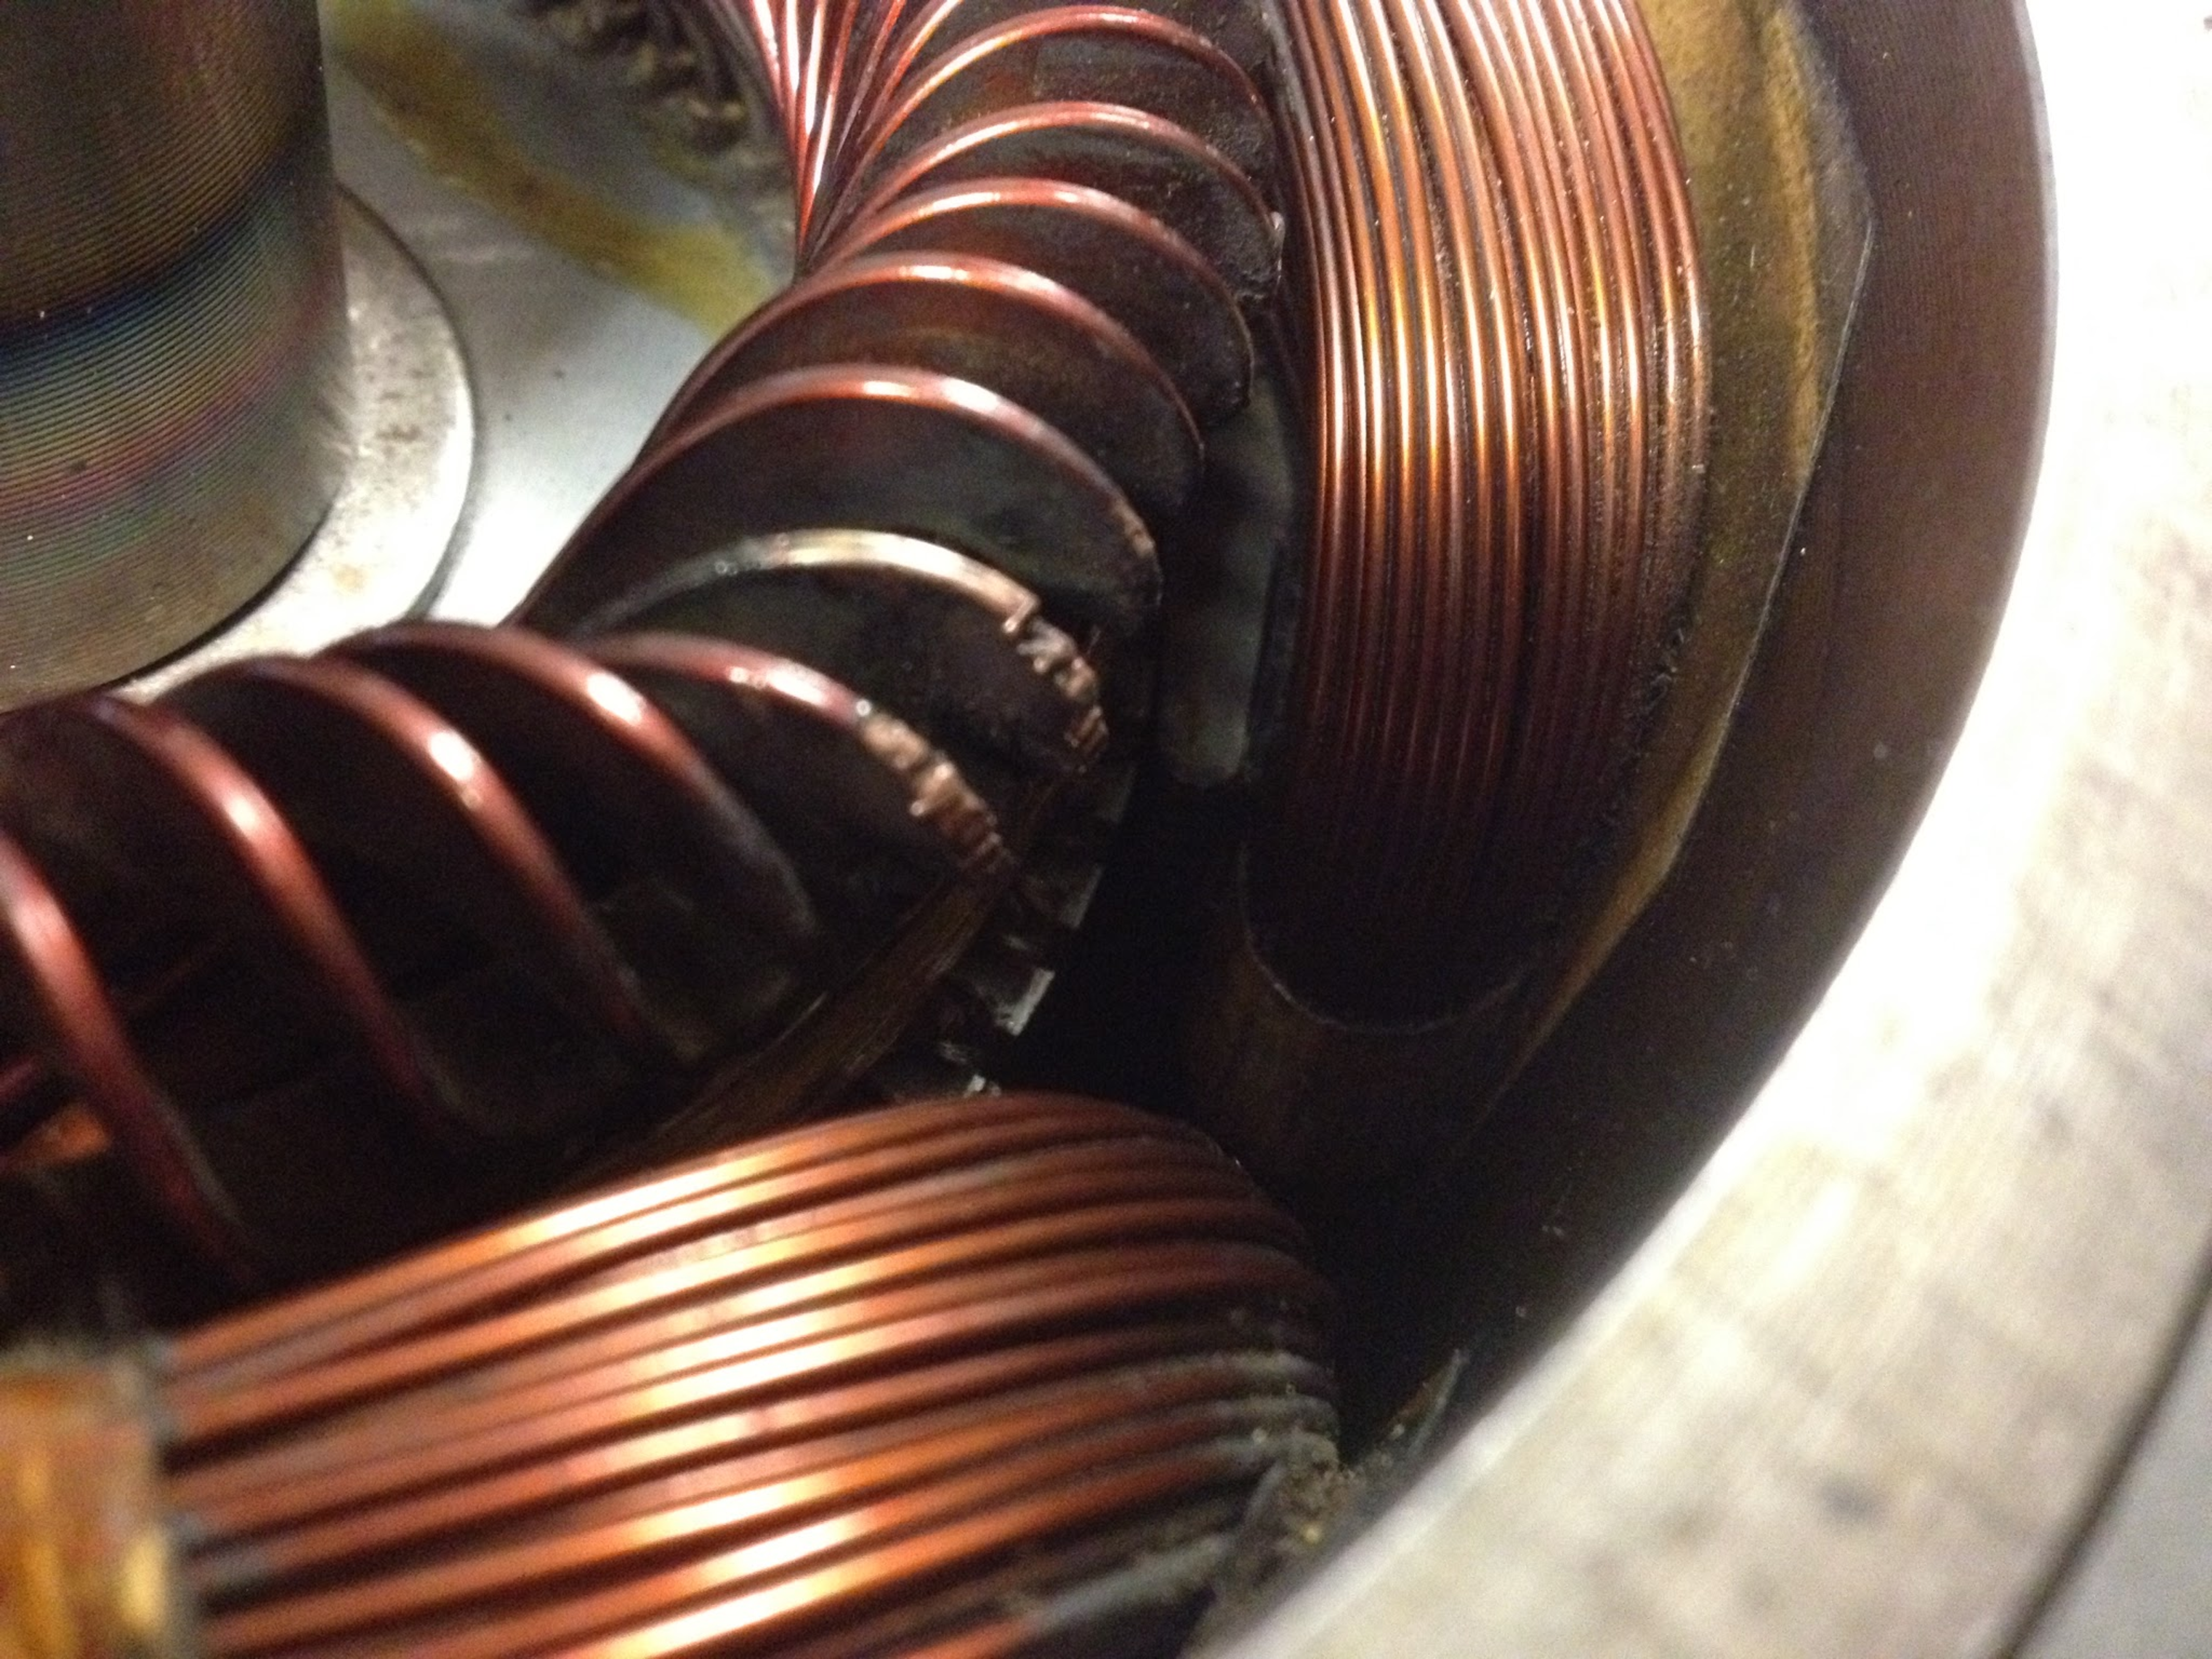
\includegraphics[width=1\textwidth]{broken_winding_1.pdf}
\caption*{}
\label{broken_1}
\end{figure}
\FloatBarrier

\begin{figure}[!htb]
\centering
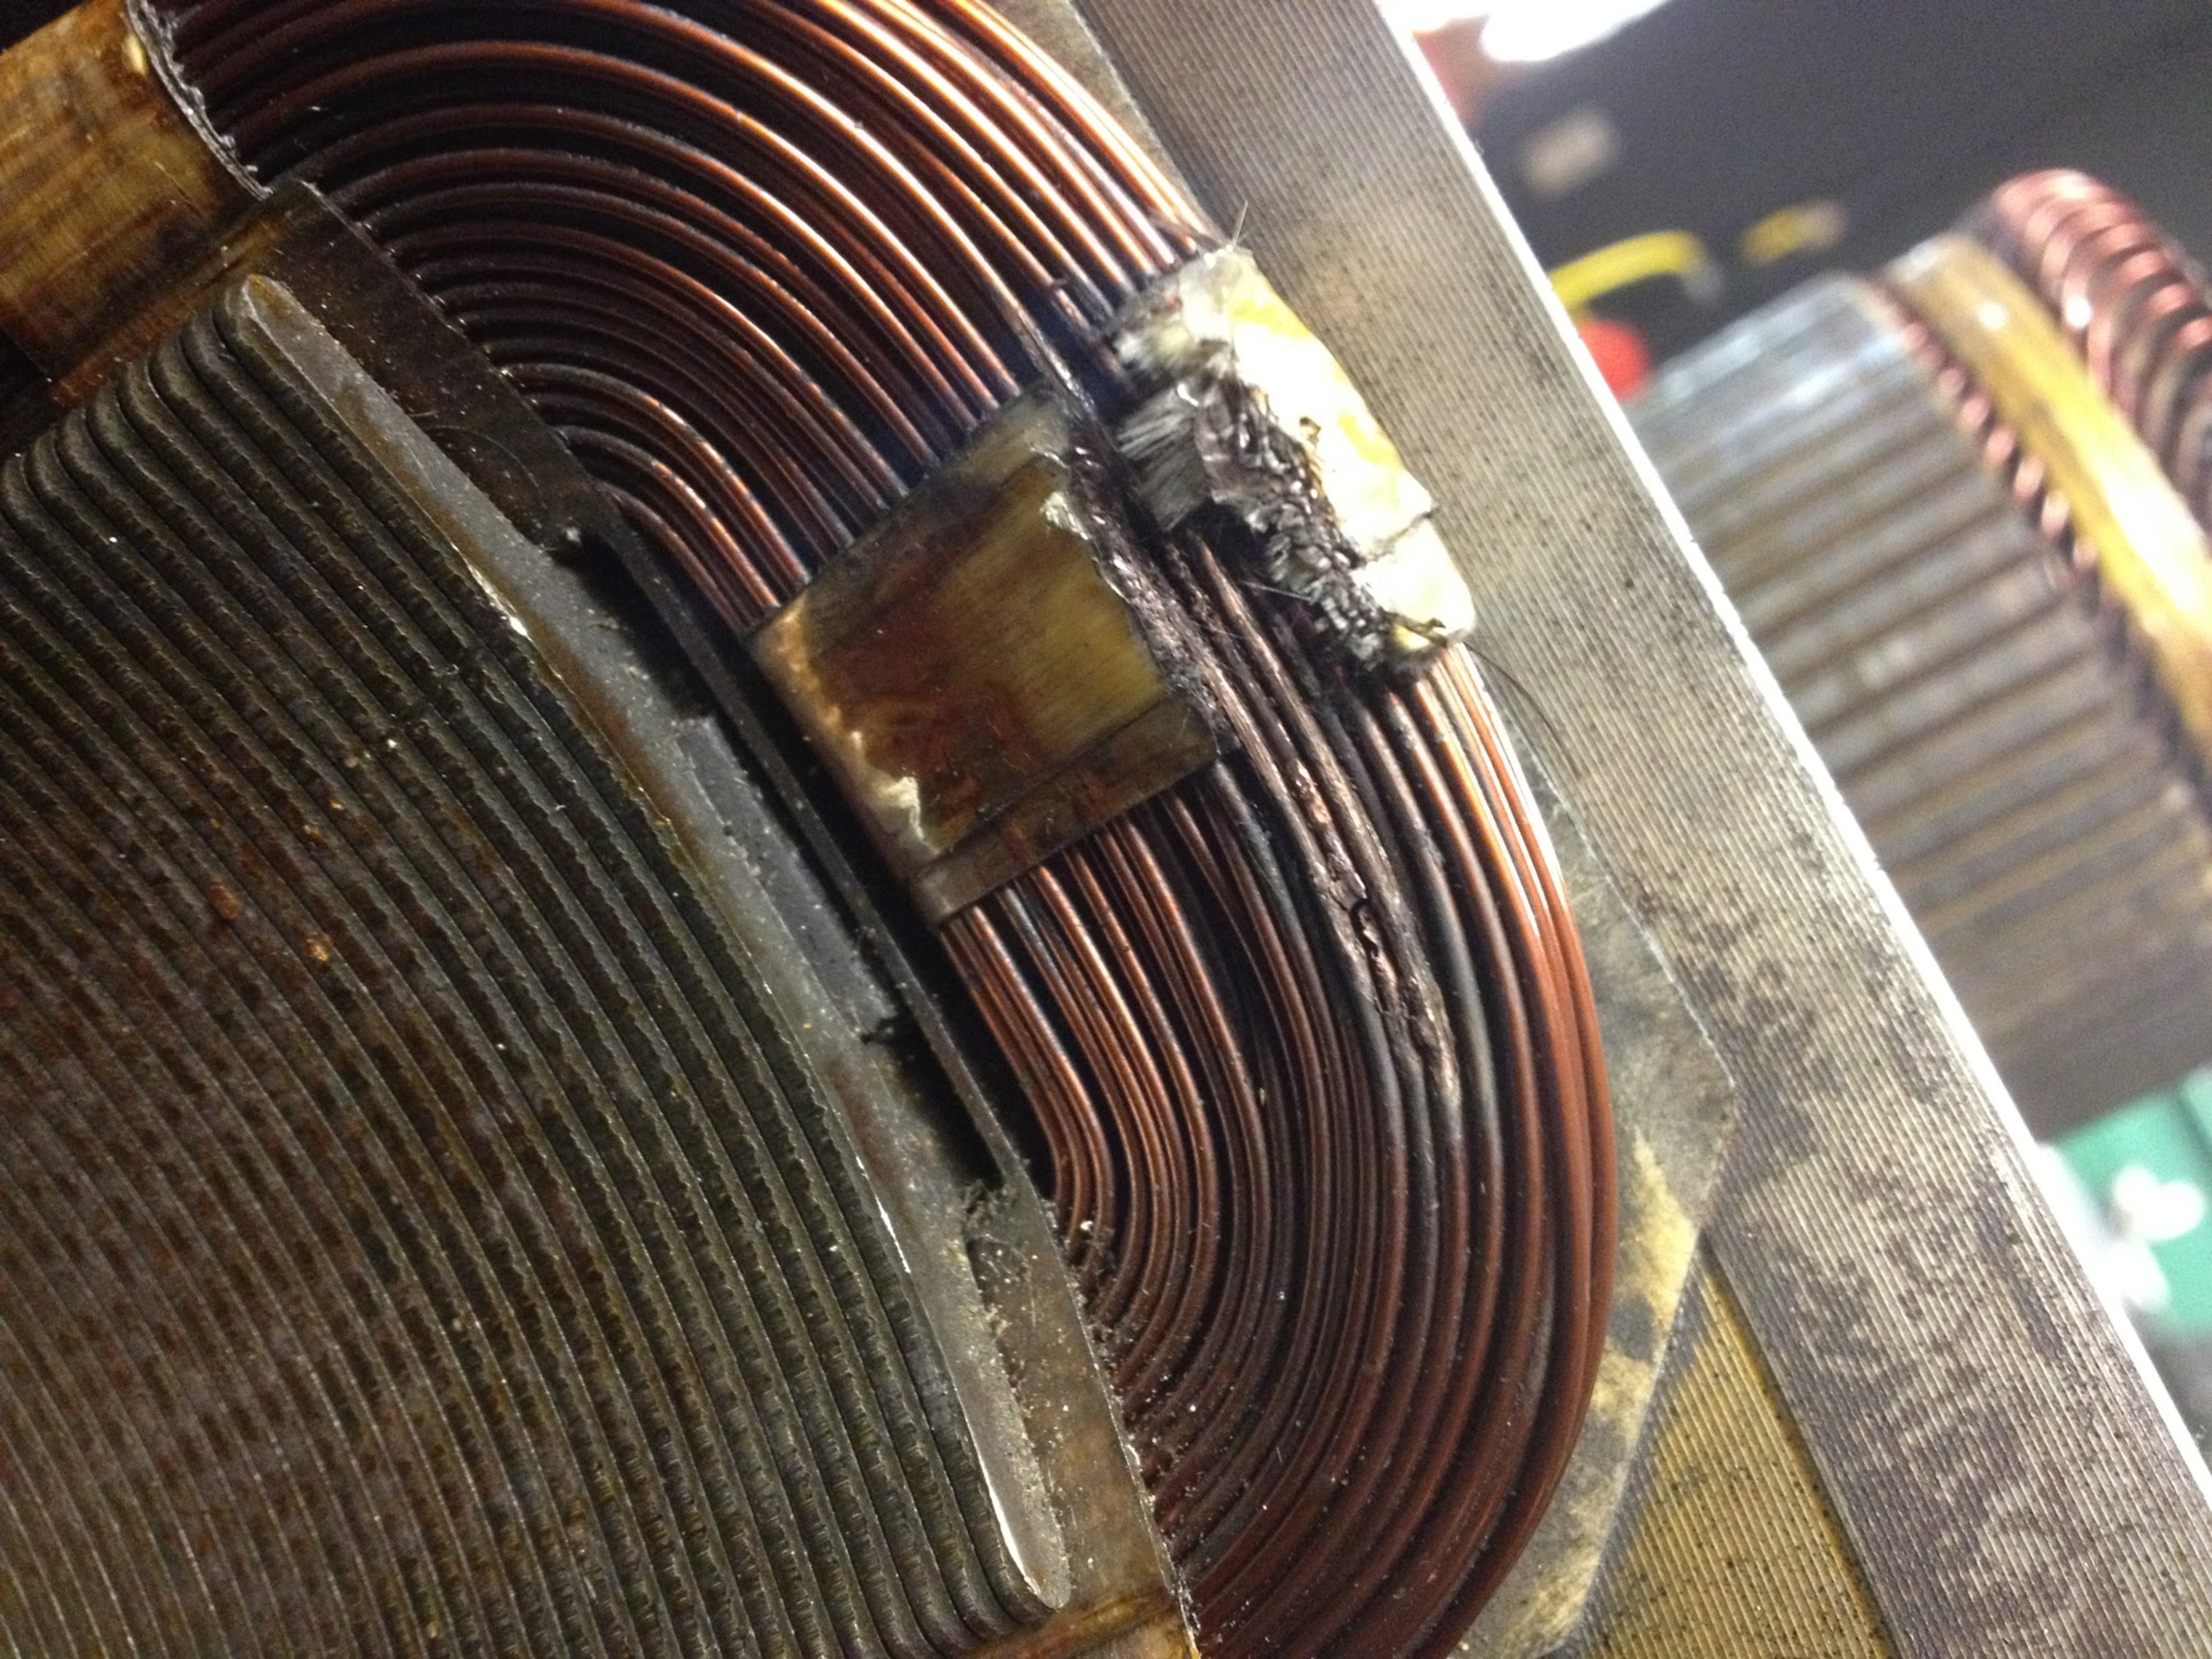
\includegraphics[width=1\textwidth]{broken_winding_2.pdf}
\caption*{}
\label{broken_2}
\end{figure}
\FloatBarrier


%////////////////////////////////////////////////////////////////////////////////////////////////////////////////////////////////////////////////////////////////////////////////////////////////////////////////////////////////////////
% APPENDIX D
%////////////////////////////////////////////////////////////////////////////////////////////////////////////////////////////////////////////////////////////////////////////////////////////////////////////////////////////////////////
\newpage
\section{Code Reference}

\begin{figure}[!htb]
\centering
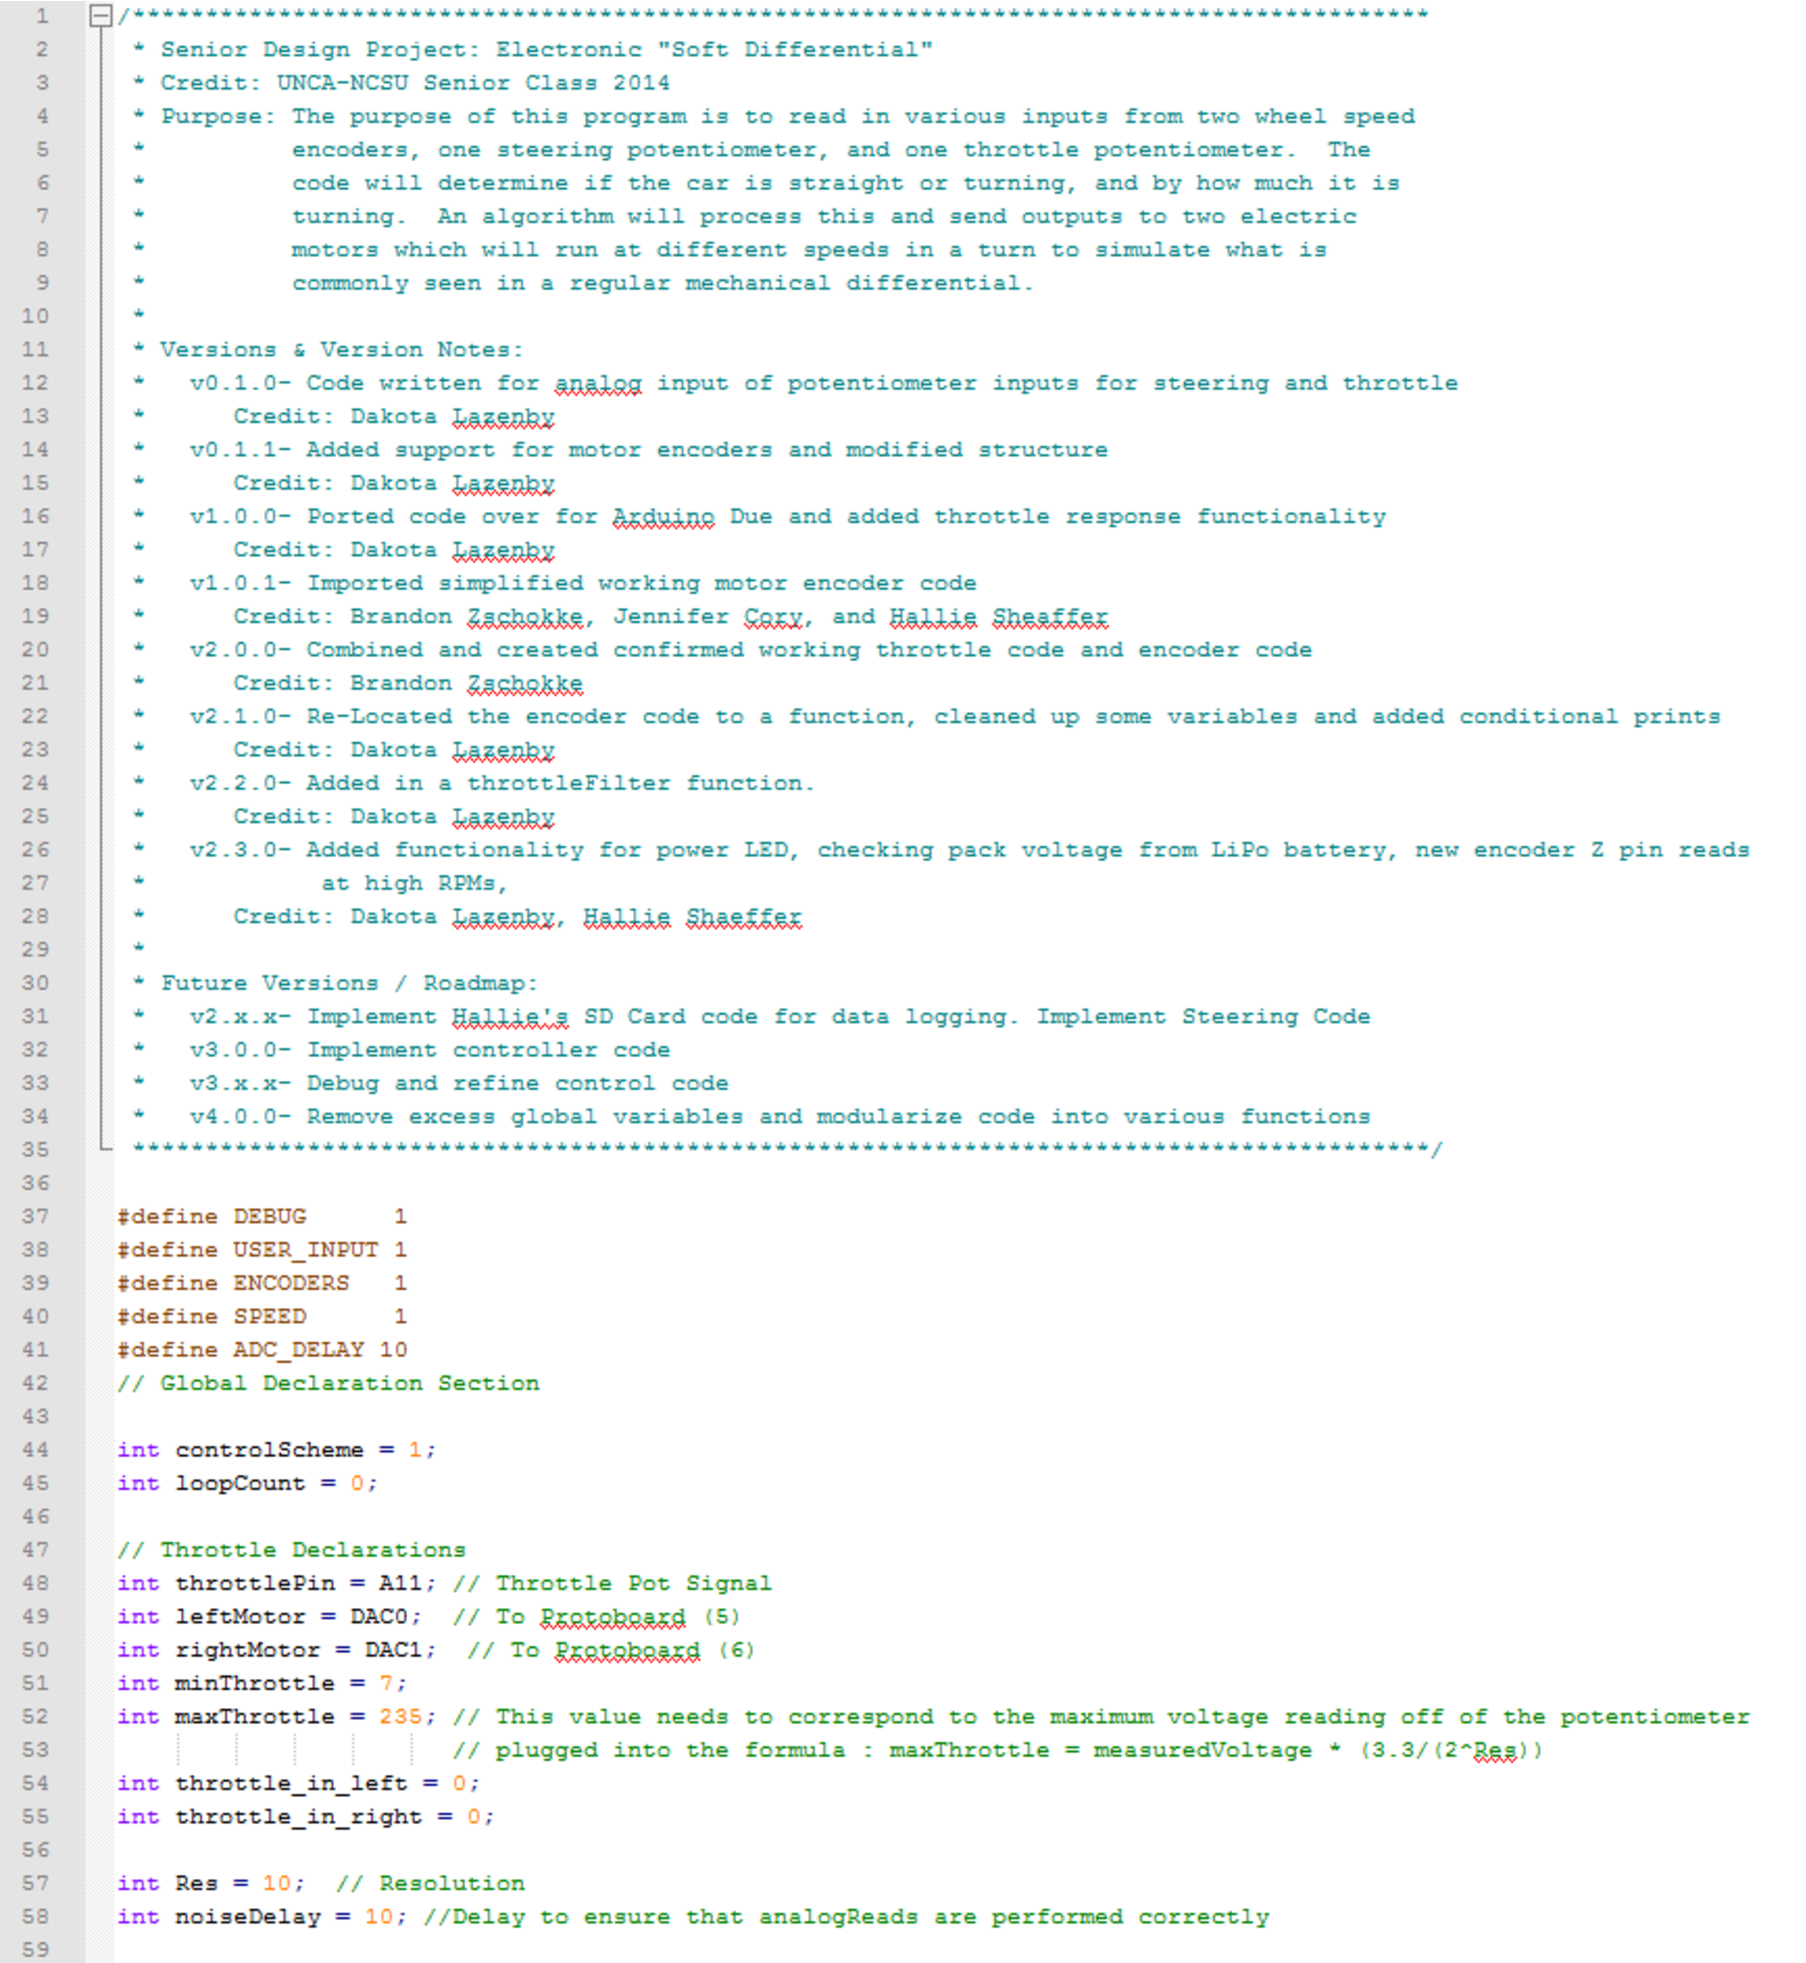
\includegraphics[width=1\textwidth]{code_1.pdf}
\caption*{}
\label{code_1}
\end{figure}
\FloatBarrier

\begin{figure}[!htb]
\centering
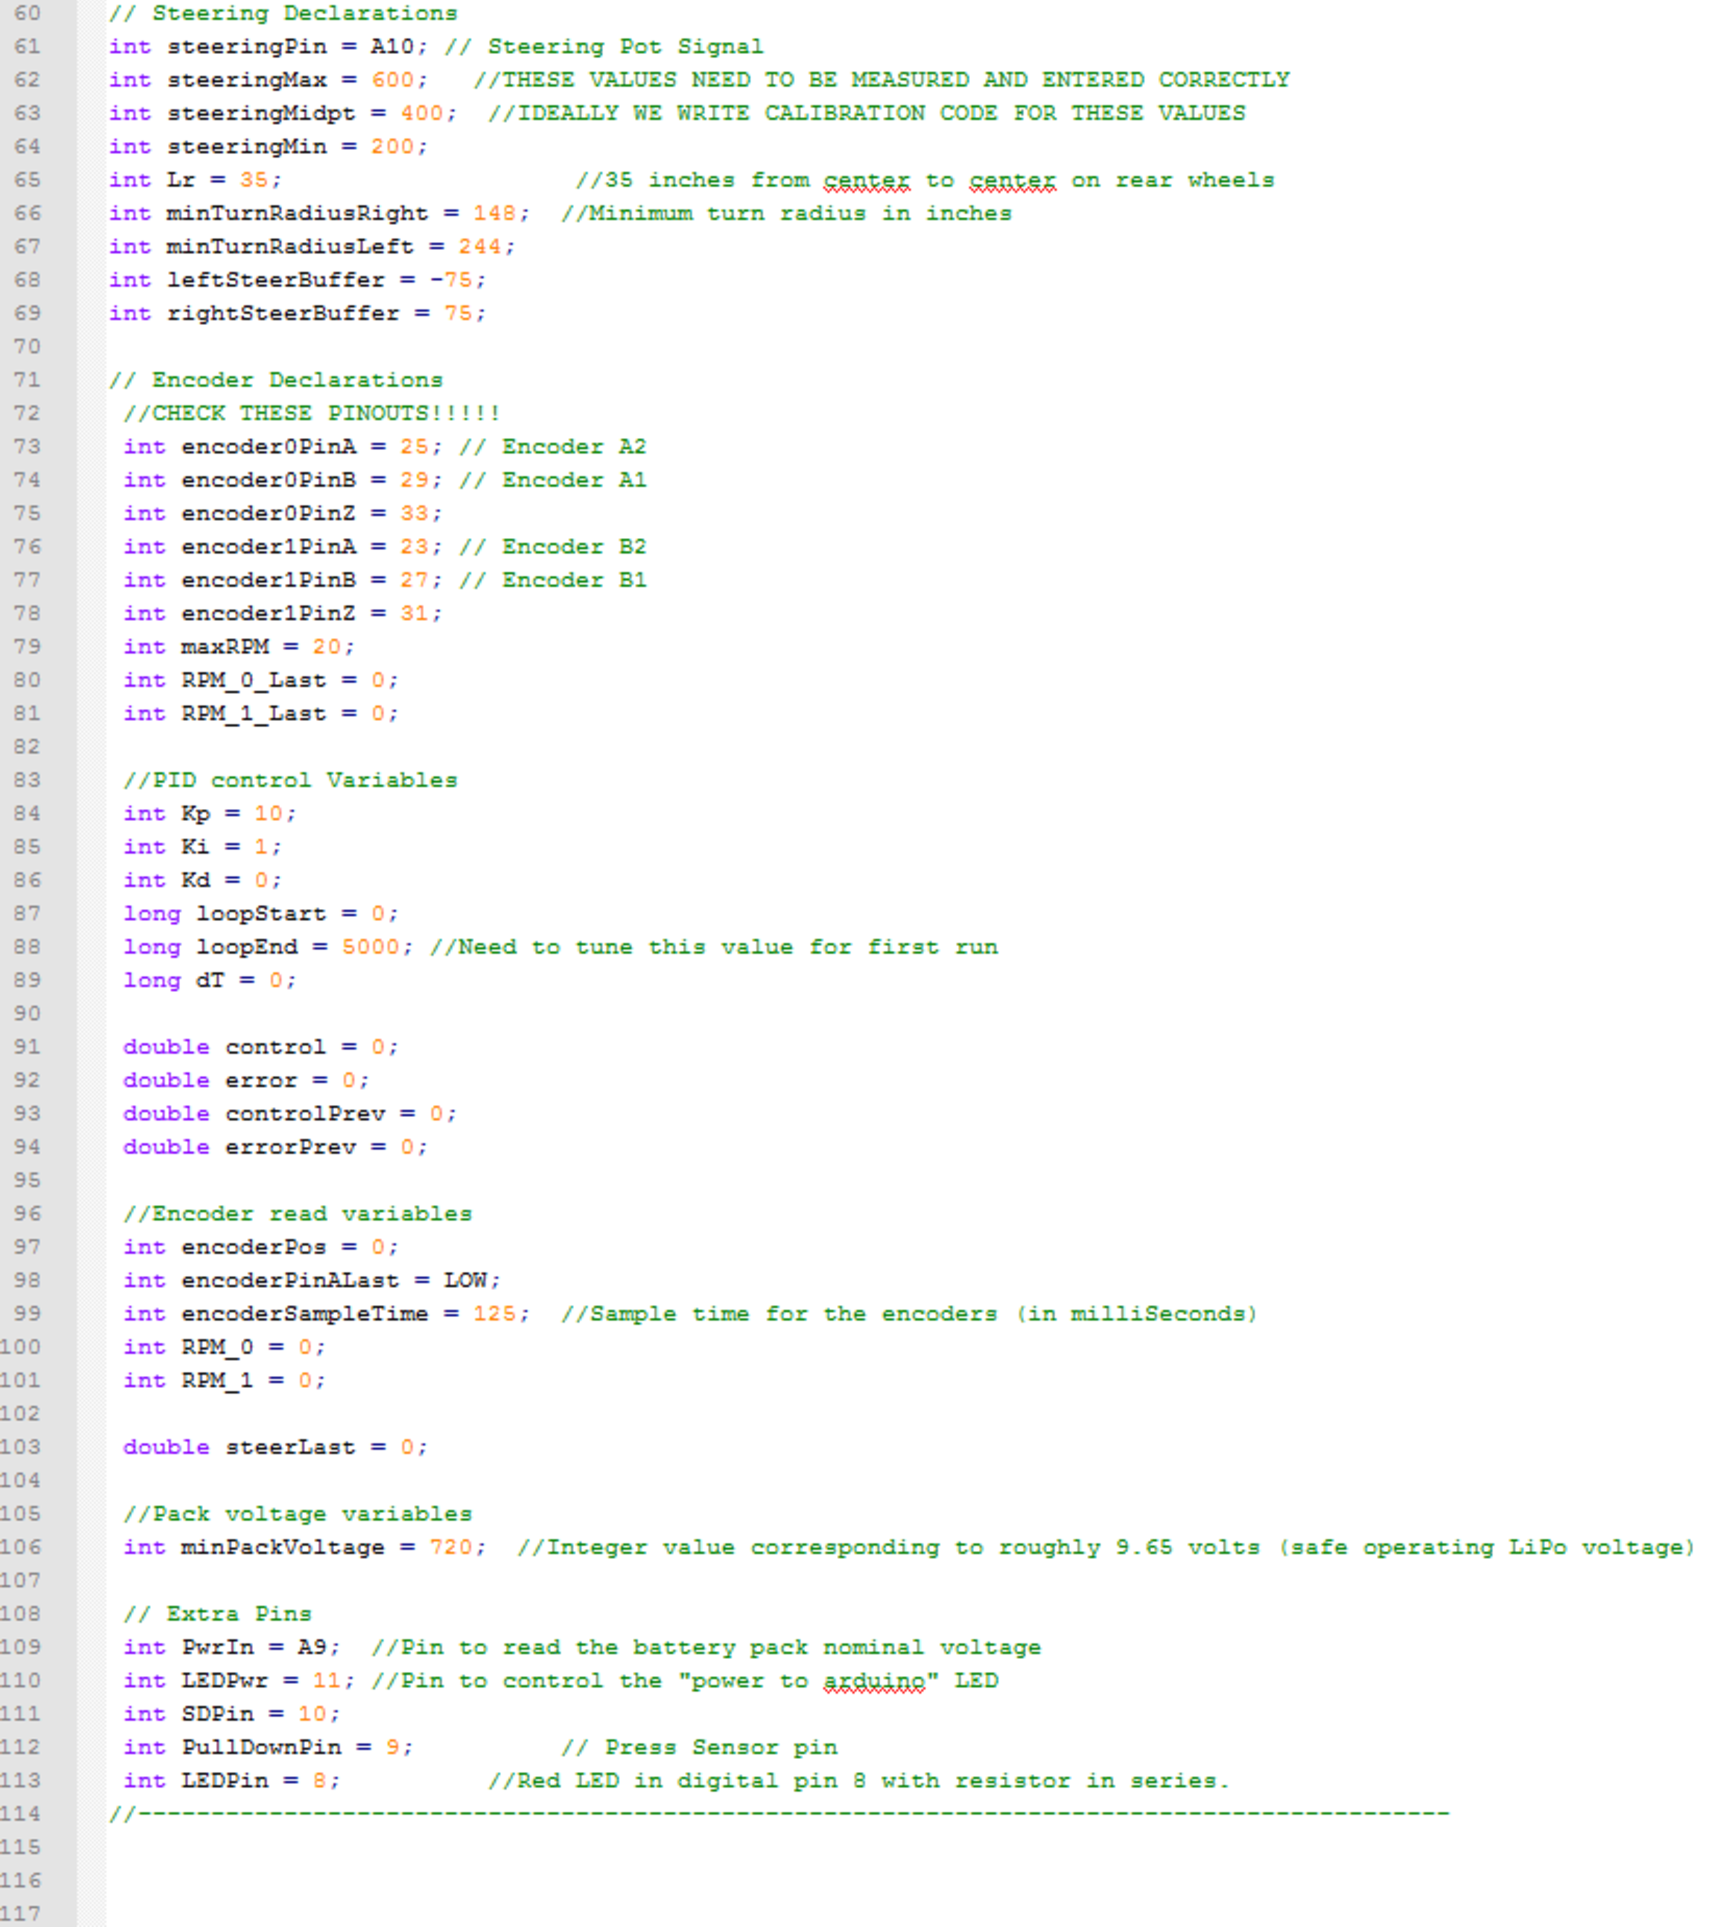
\includegraphics[width=1\textwidth]{code_2.pdf}
\caption*{}
\label{code_2}
\end{figure}
\FloatBarrier

\begin{figure}[!htb]
\centering
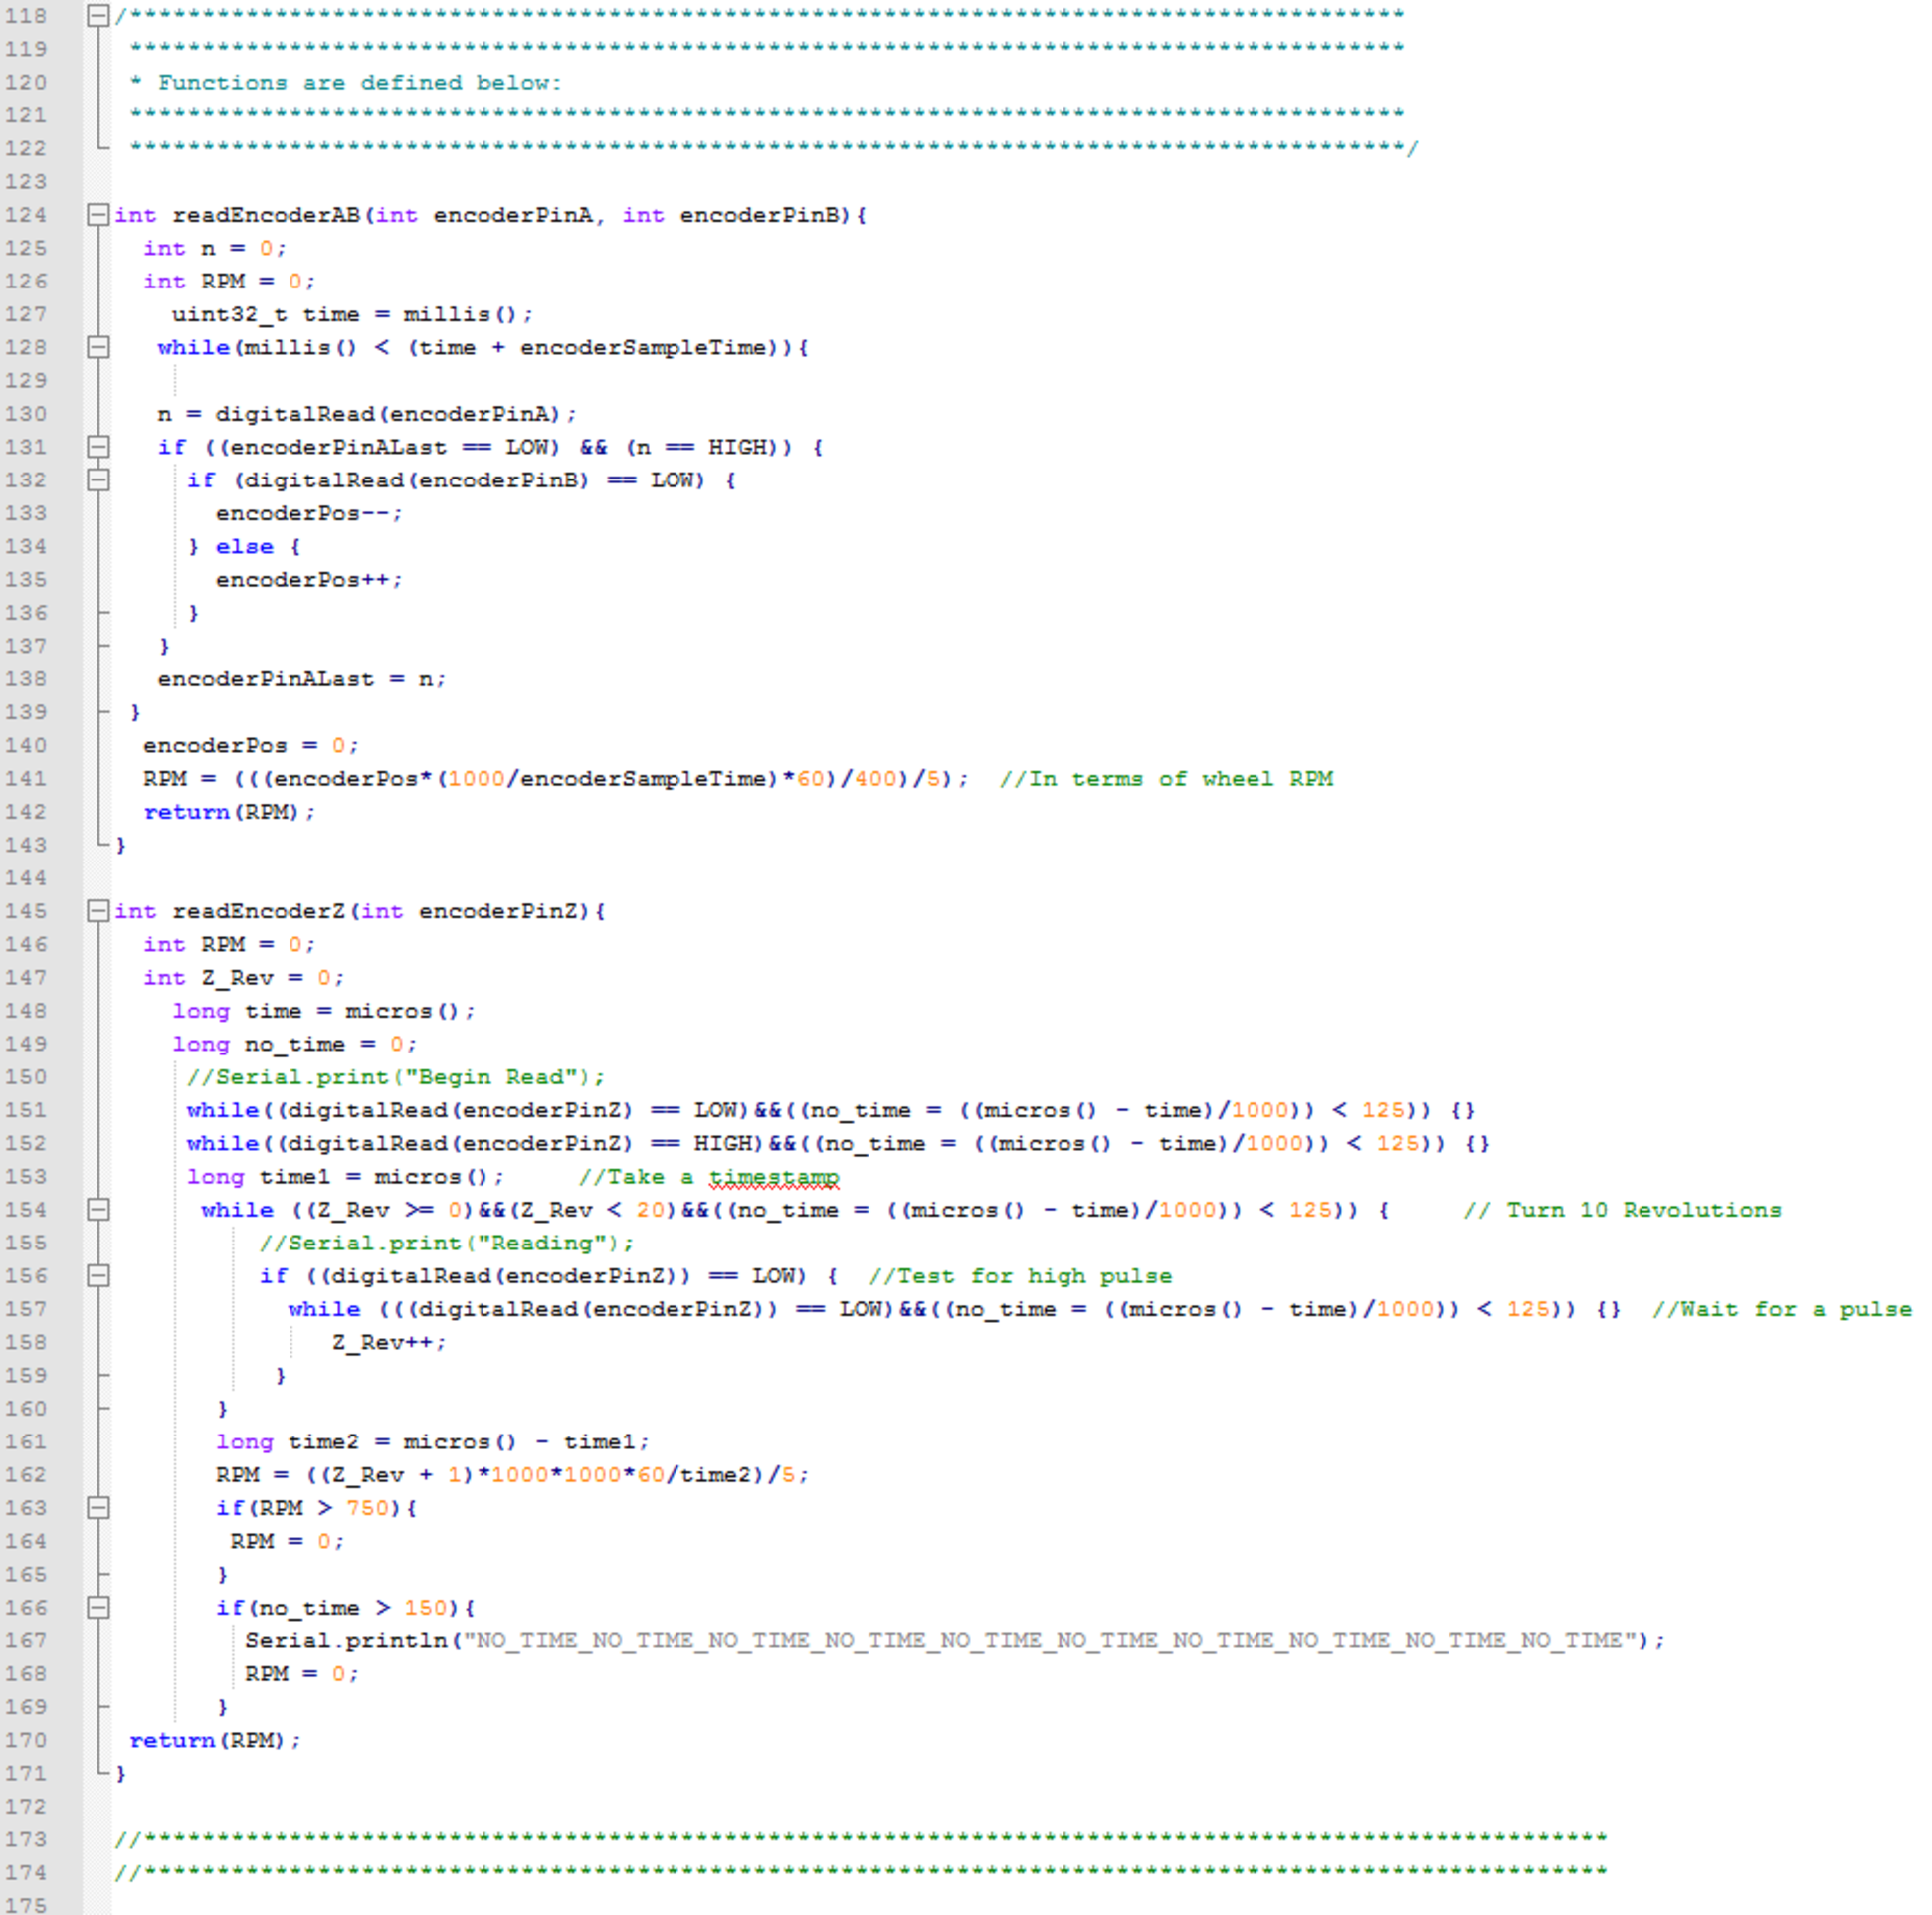
\includegraphics[width=1\textwidth]{code_3.pdf}
\caption*{}
\label{code_3}
\end{figure}
\FloatBarrier

\begin{figure}[!htb]
\centering
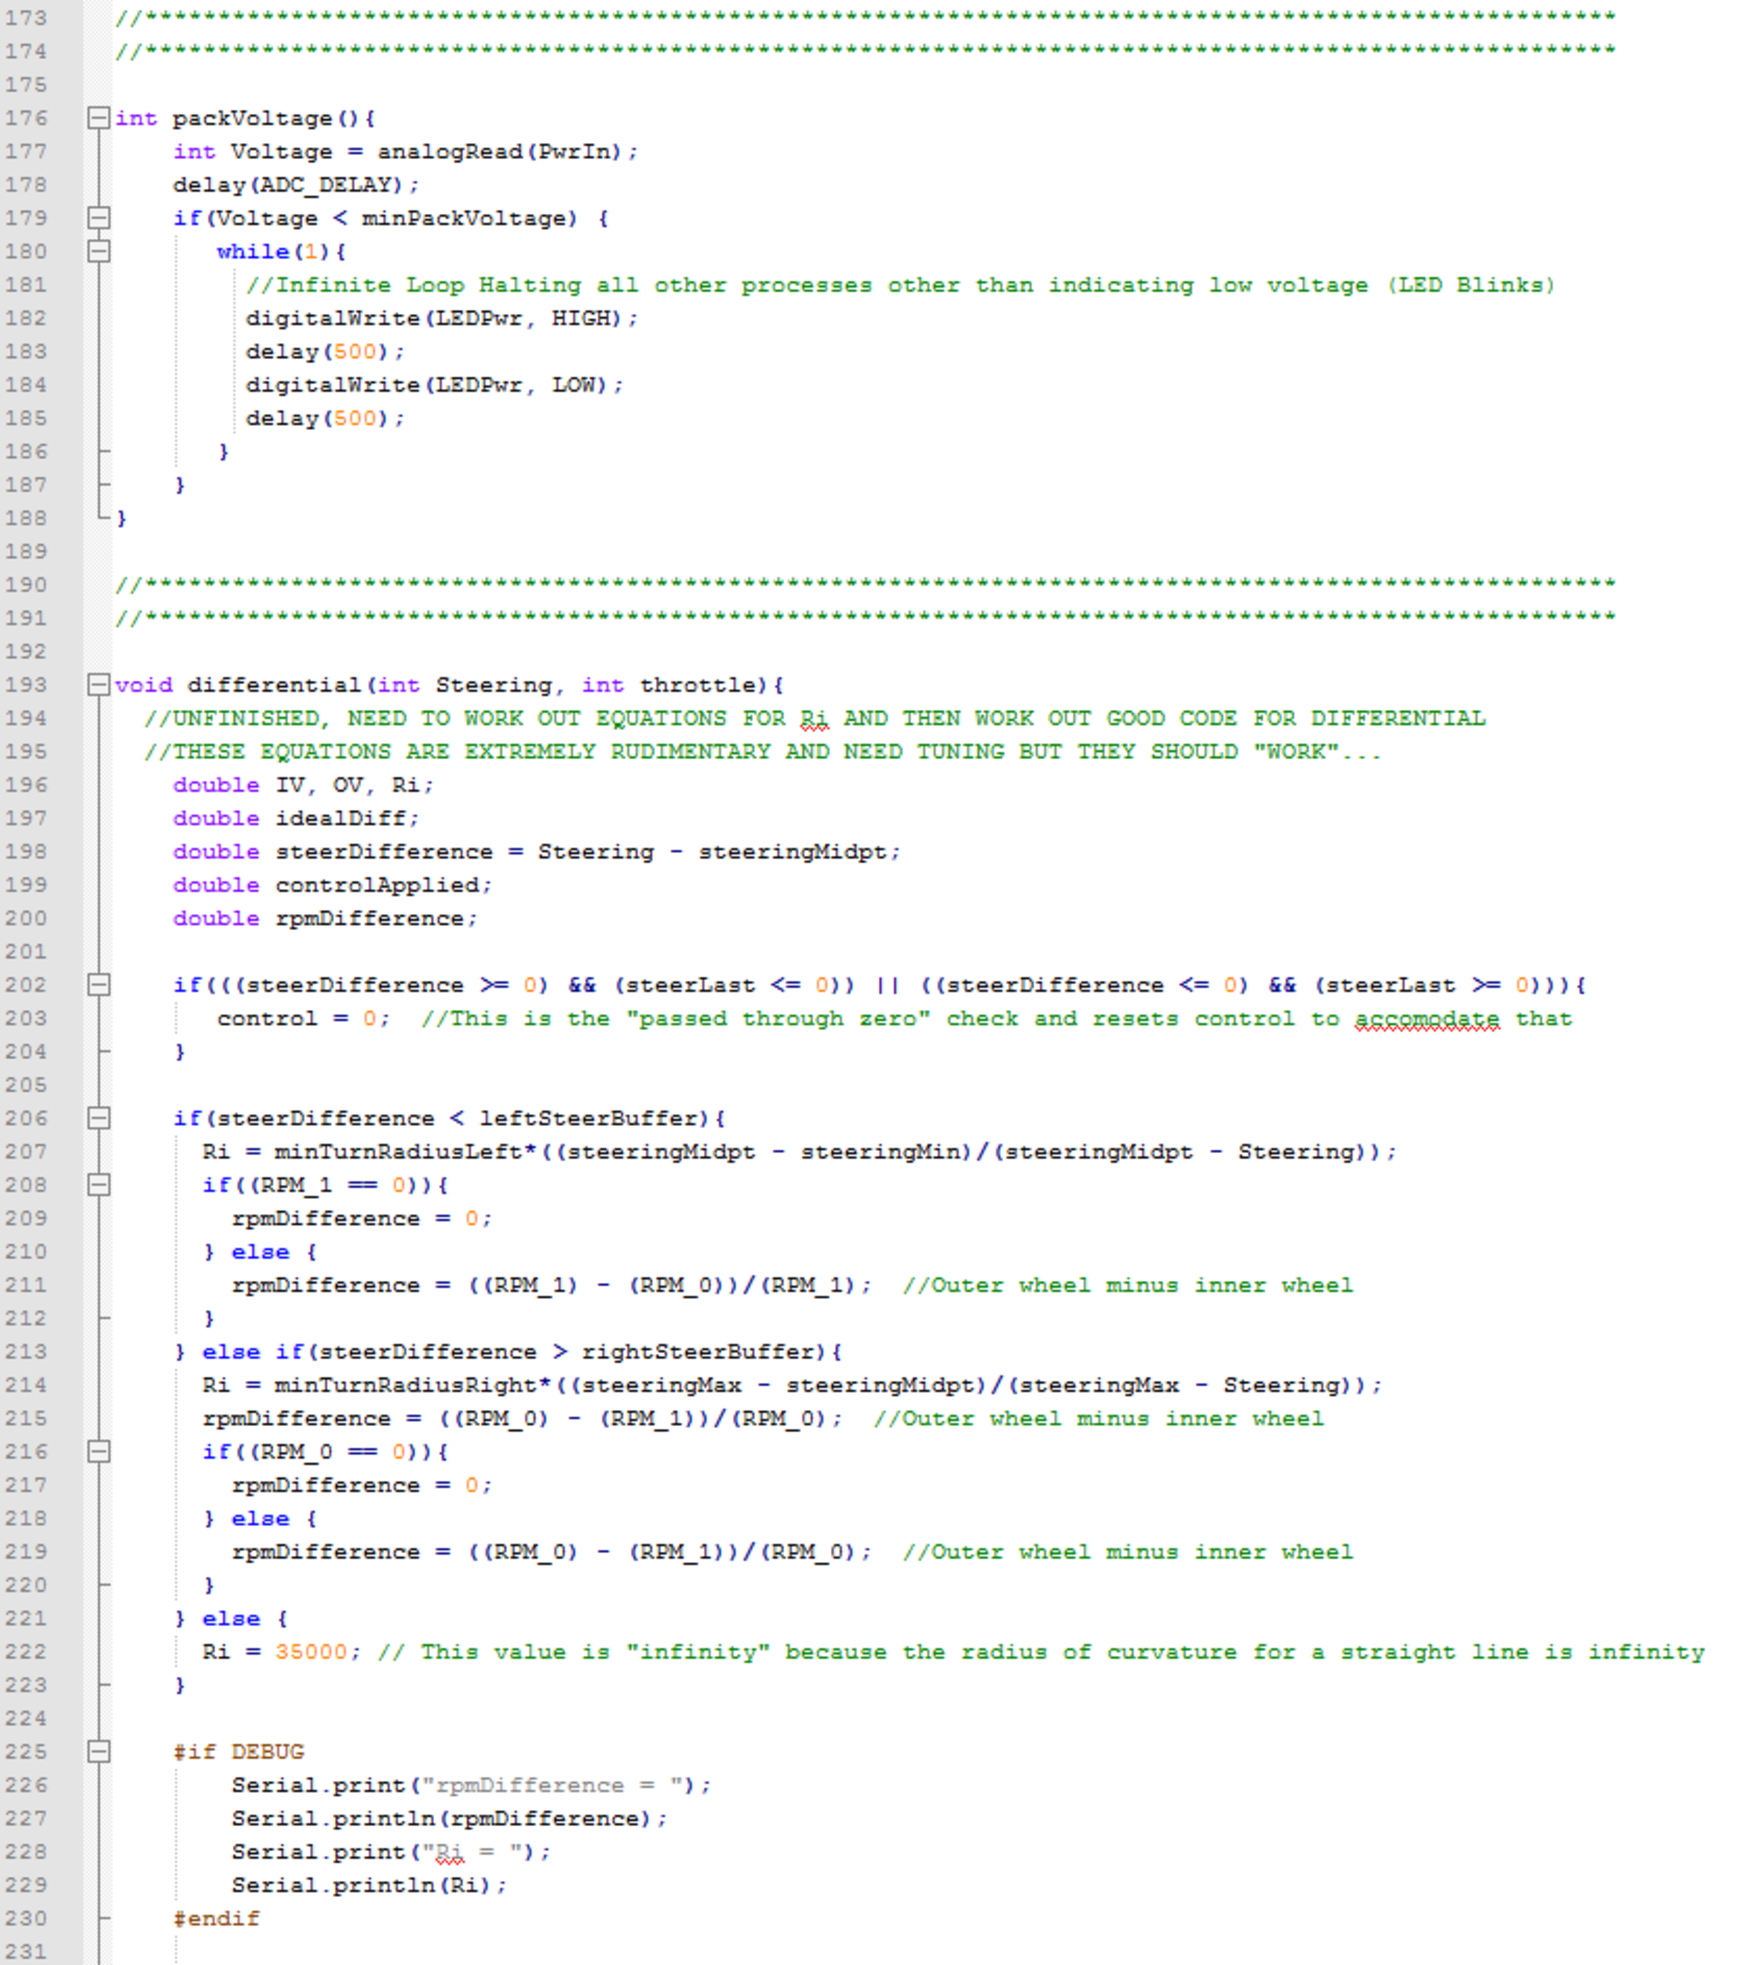
\includegraphics[width=1\textwidth]{code_4.pdf}
\caption*{}
\label{code_4}
\end{figure}
\FloatBarrier

\begin{figure}[!htb]
\centering
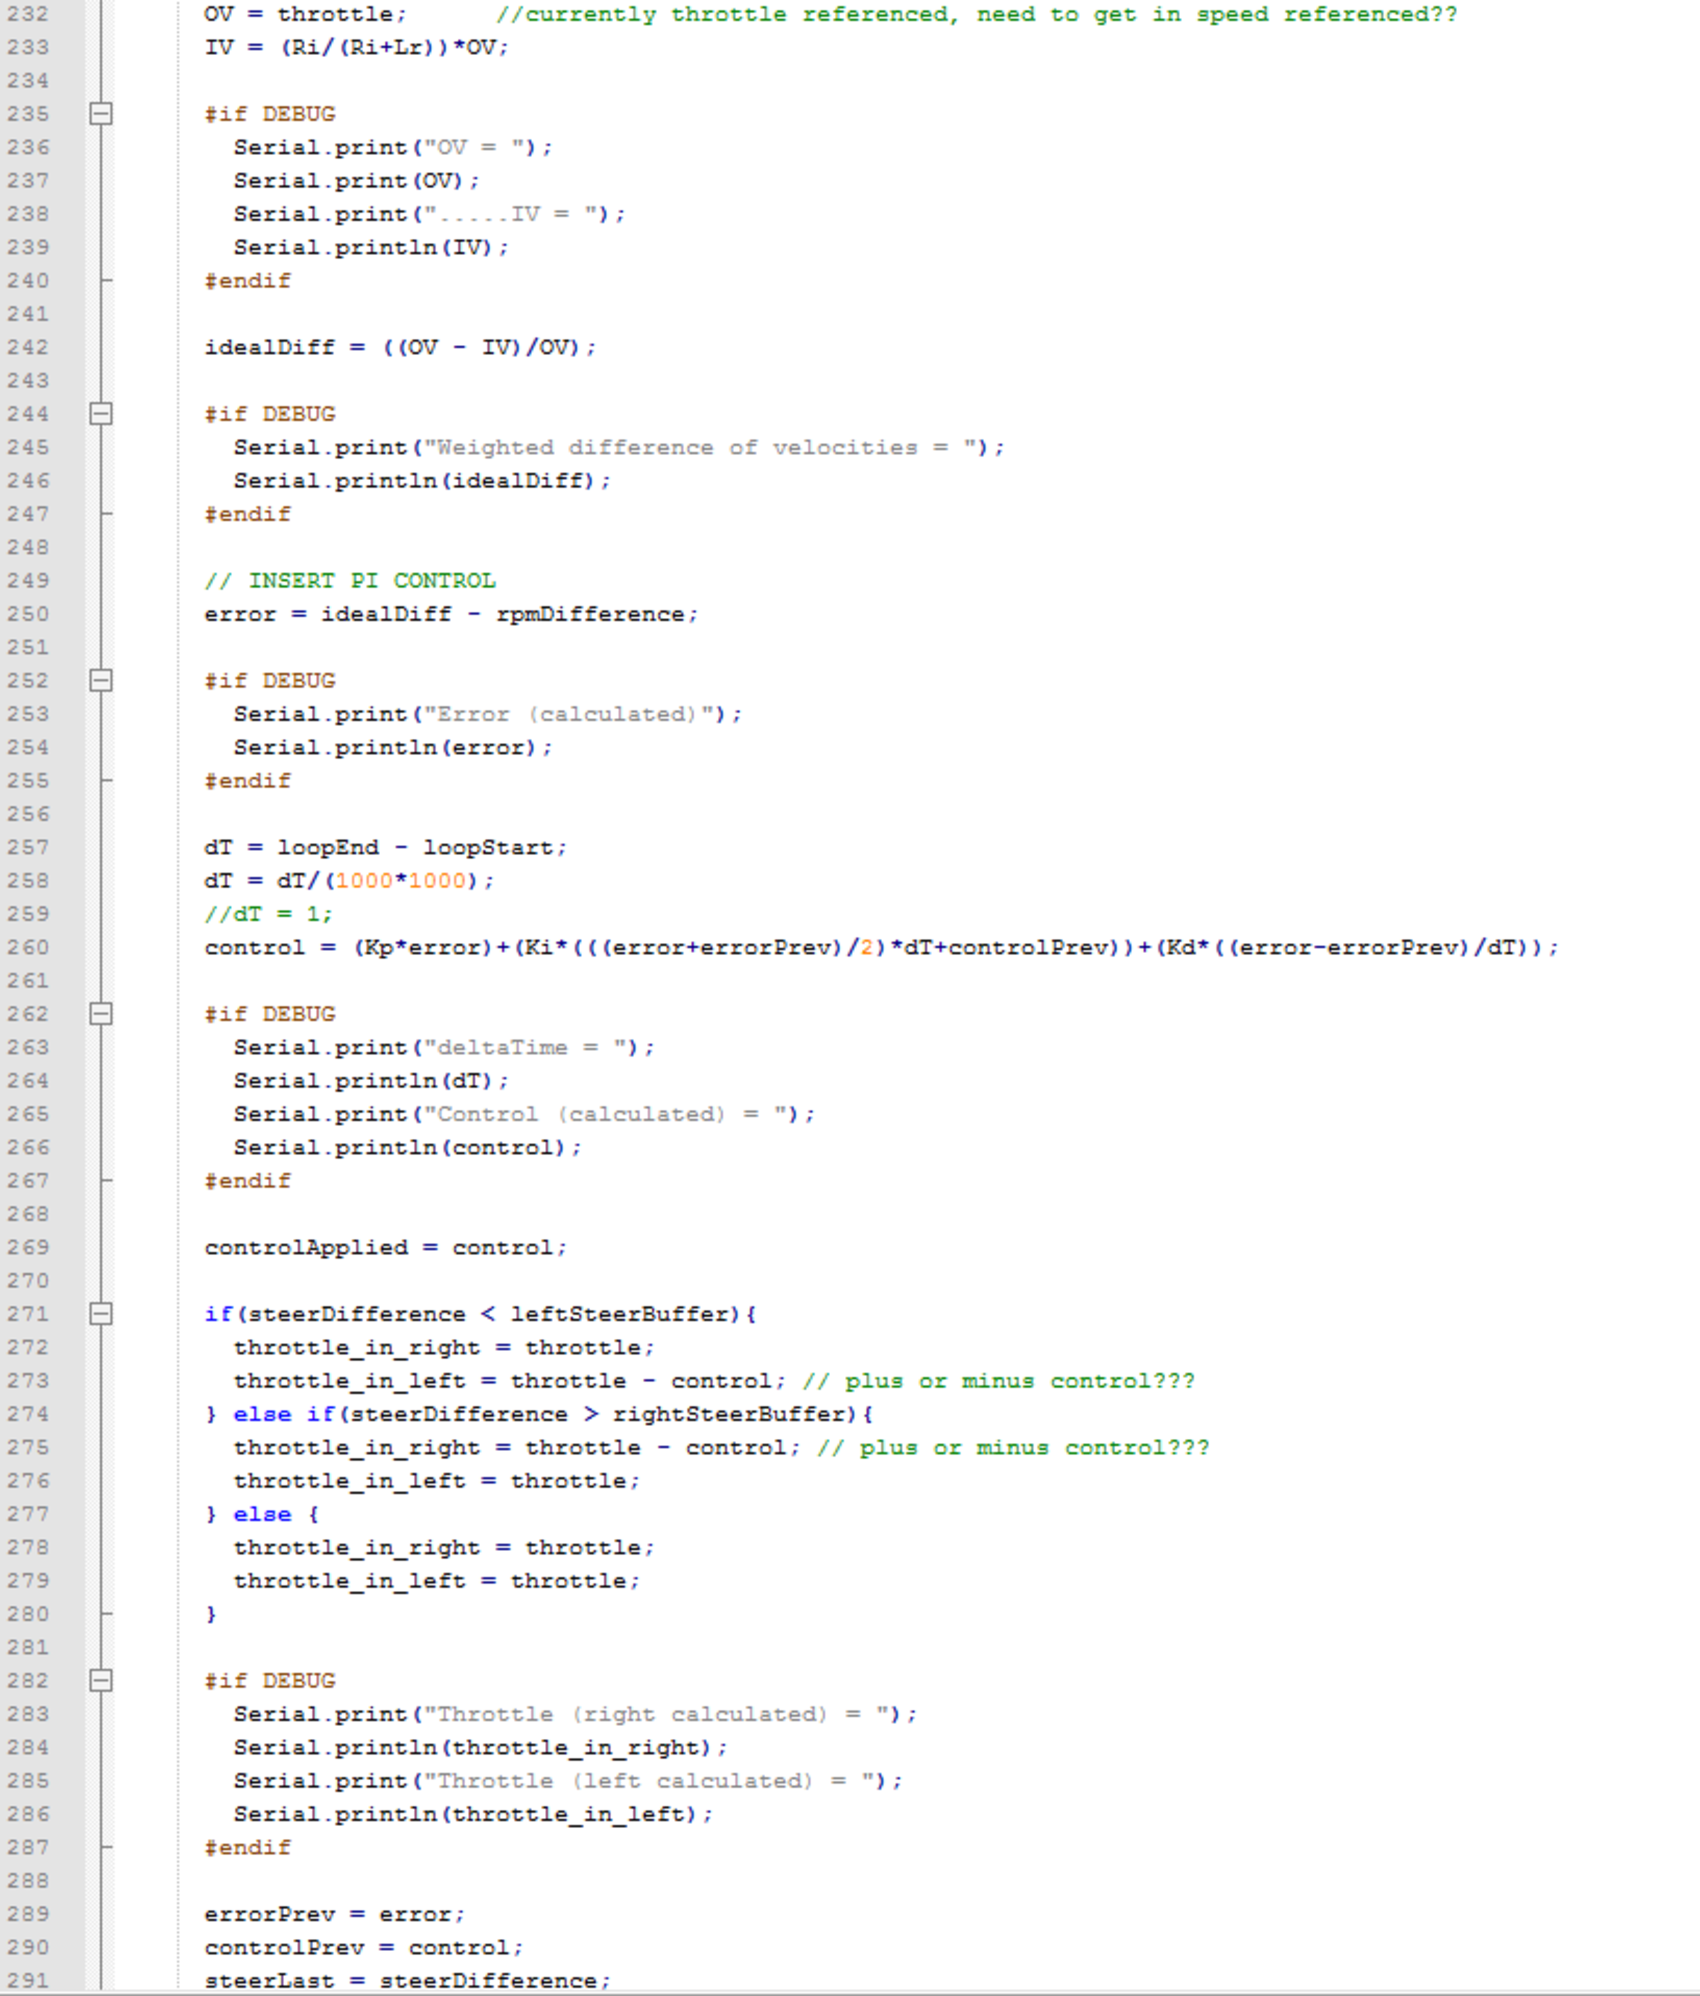
\includegraphics[width=1\textwidth]{code_5.pdf}
\caption*{}
\label{code_5}
\end{figure}
\FloatBarrier

\begin{figure}[!htb]
\centering
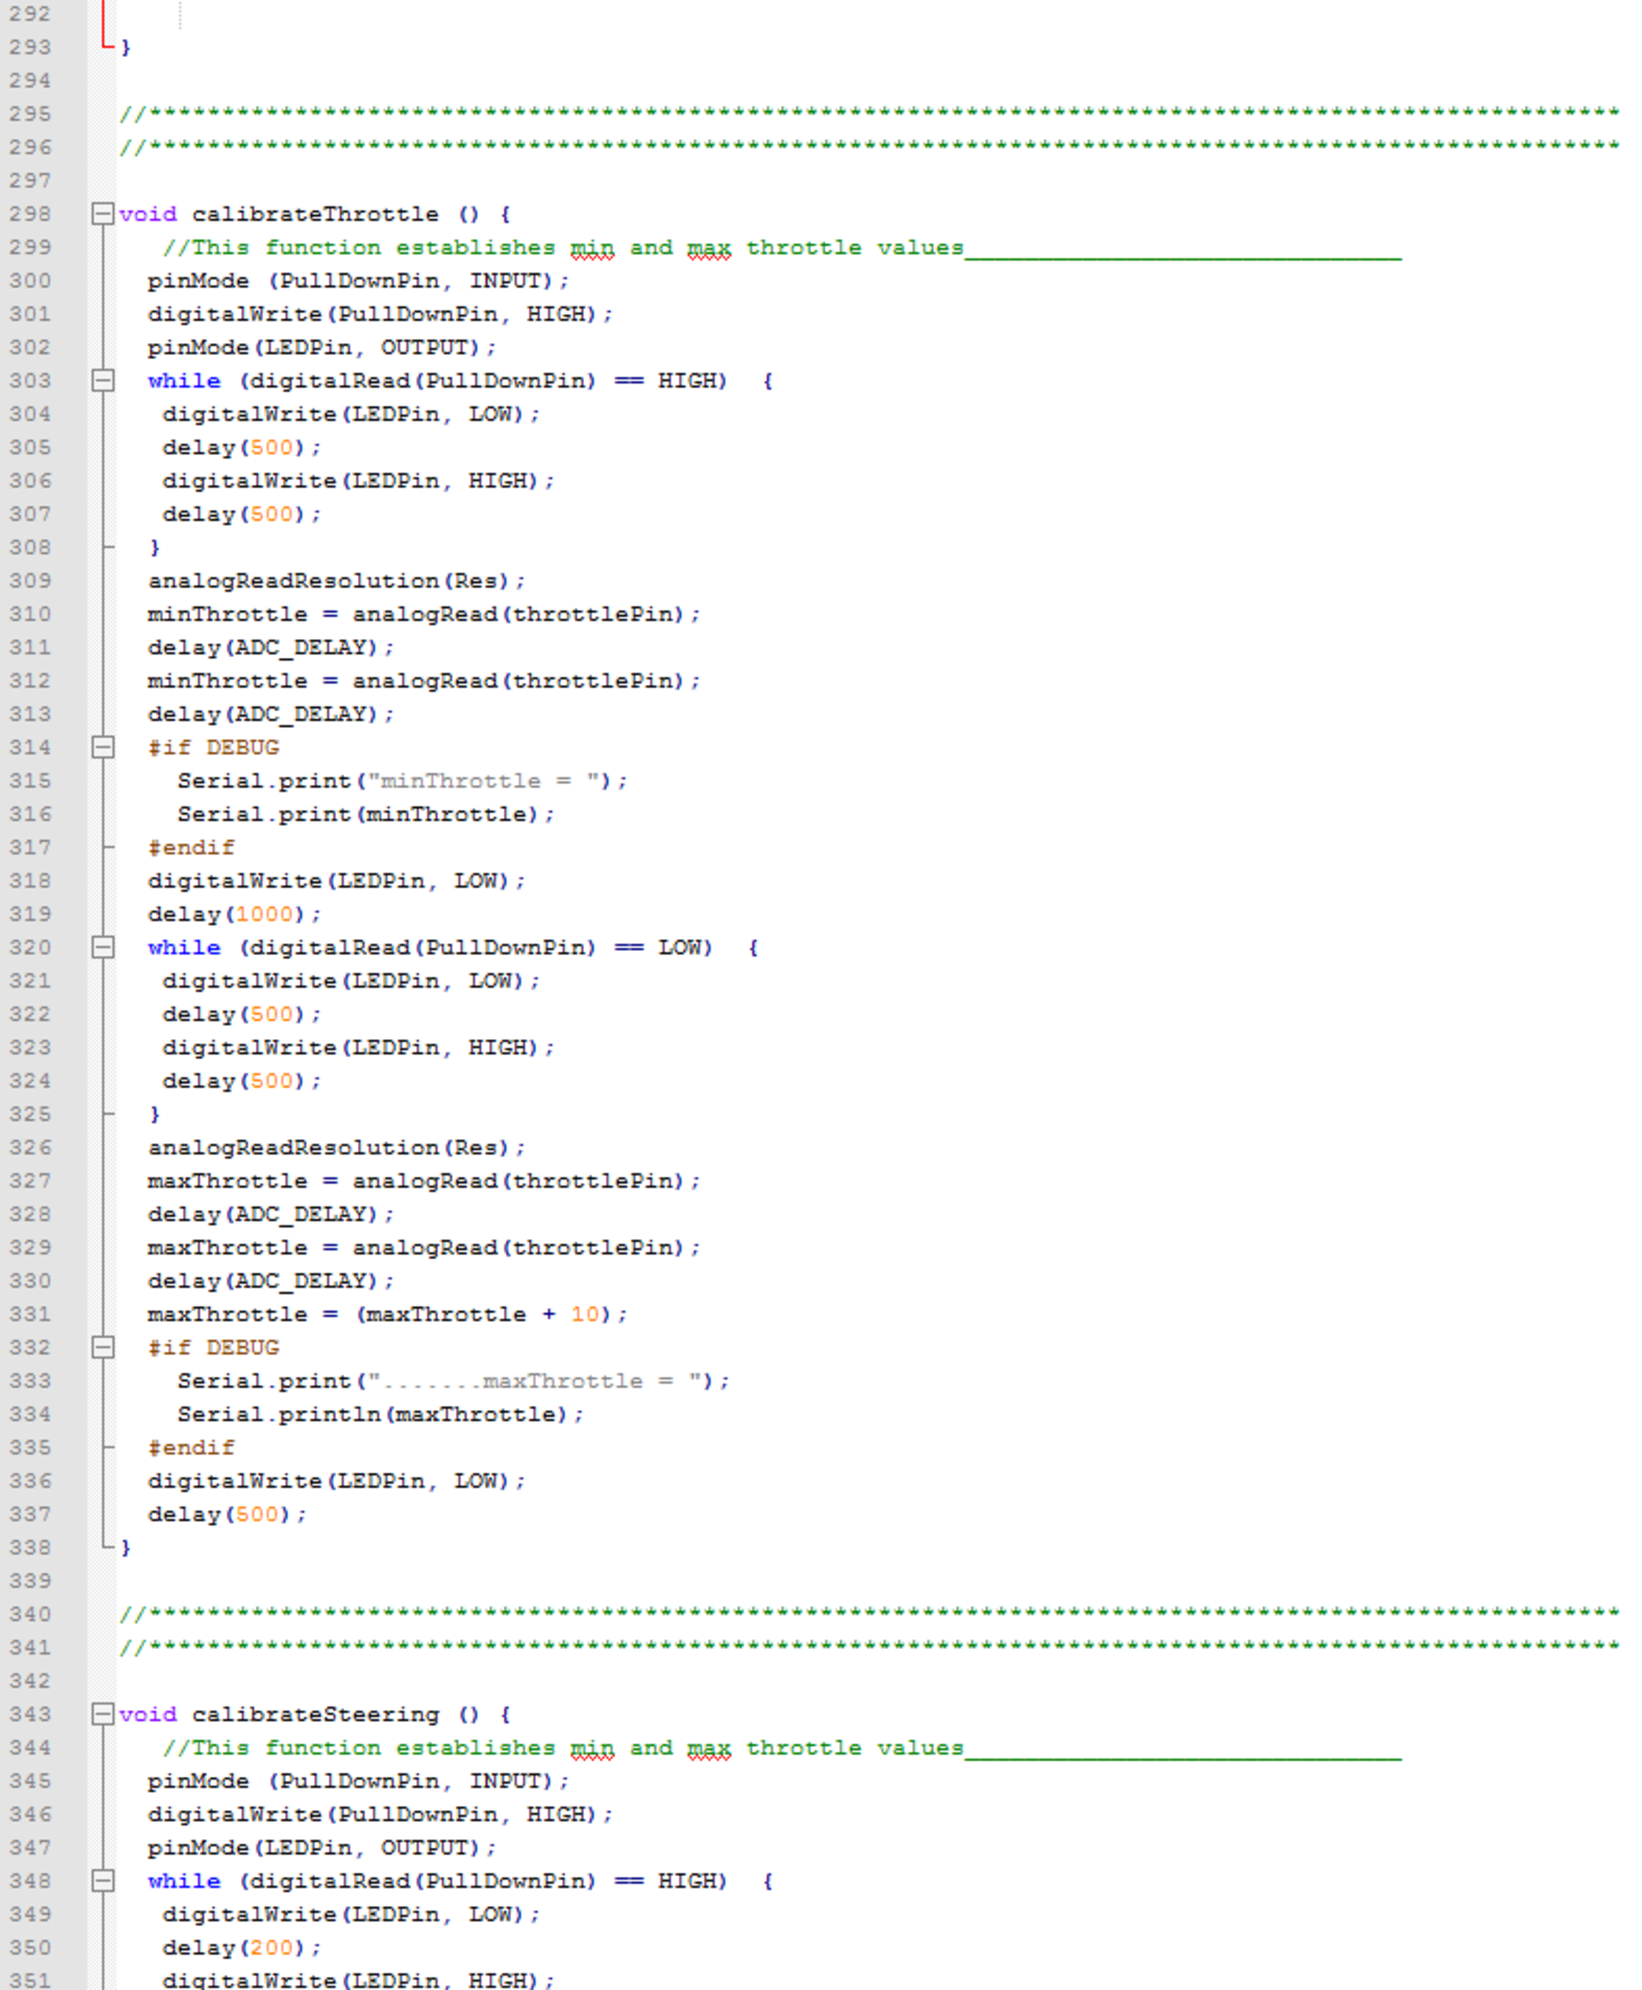
\includegraphics[width=1\textwidth]{code_6.pdf}
\caption*{}
\label{code_6}
\end{figure}
\FloatBarrier

\begin{figure}[!htb]
\centering
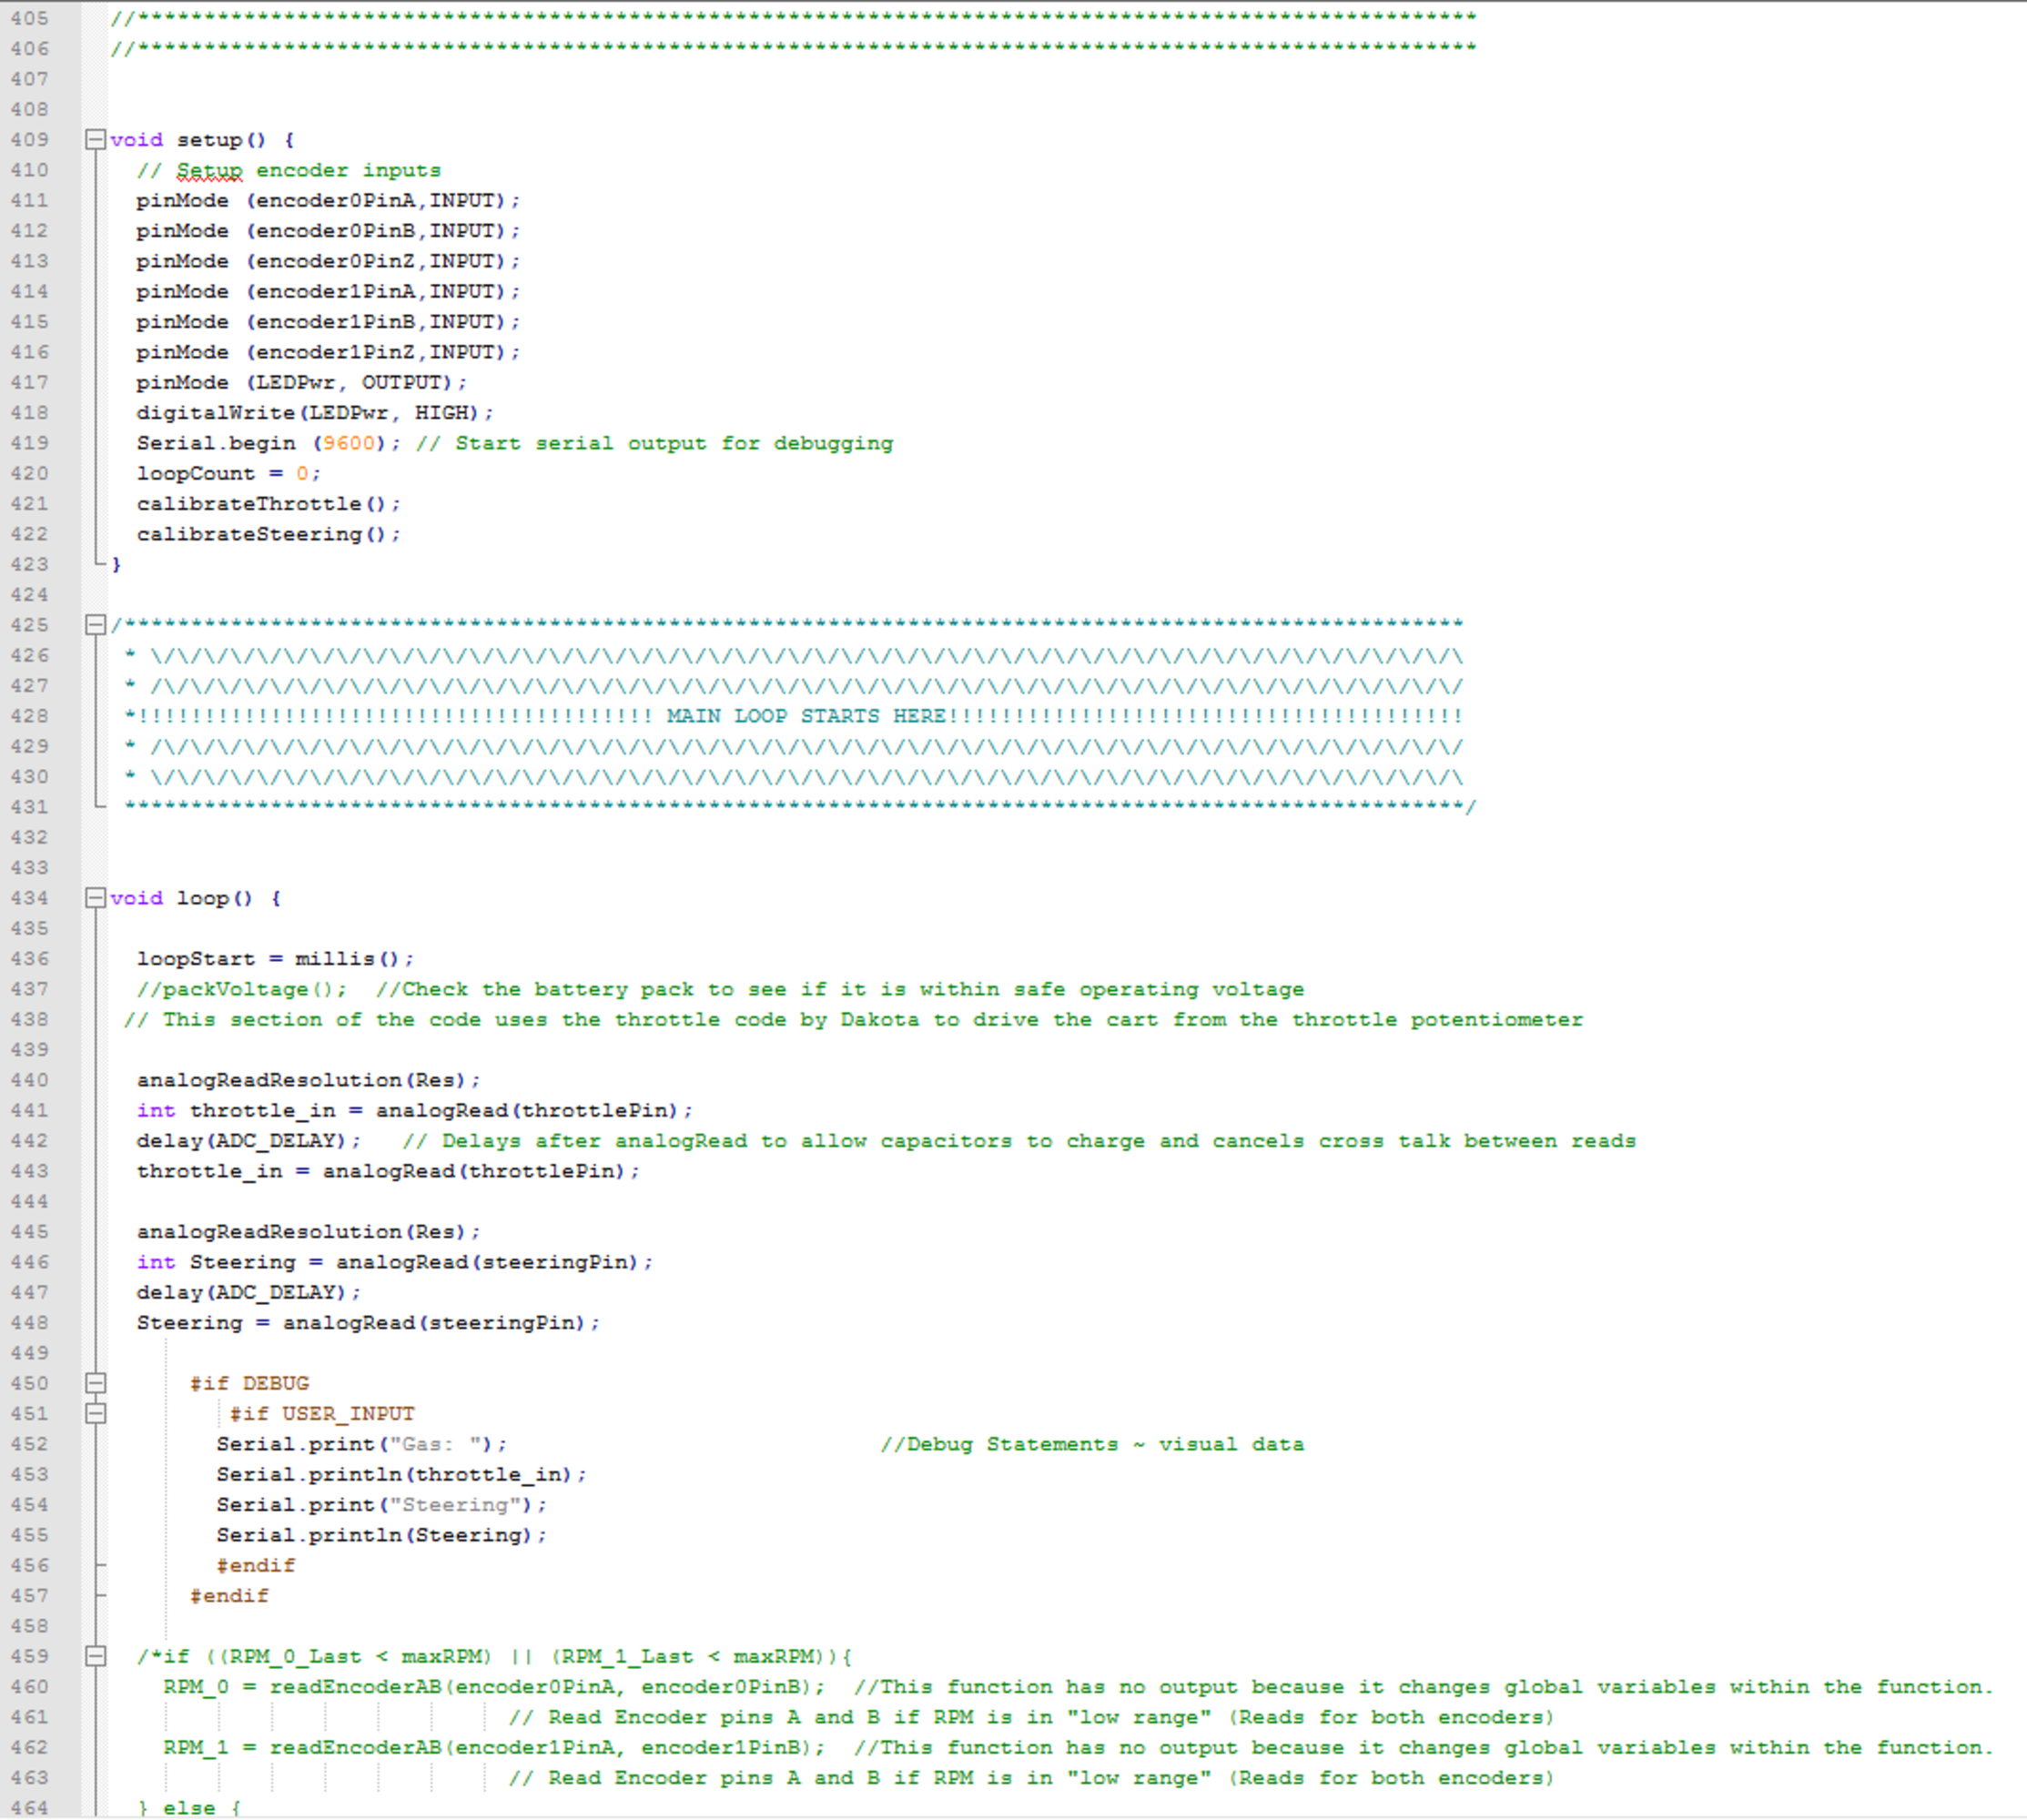
\includegraphics[width=1\textwidth]{code_7.pdf}
\caption*{}
\label{code_7}
\end{figure}
\FloatBarrier

\begin{figure}[!htb]
\centering
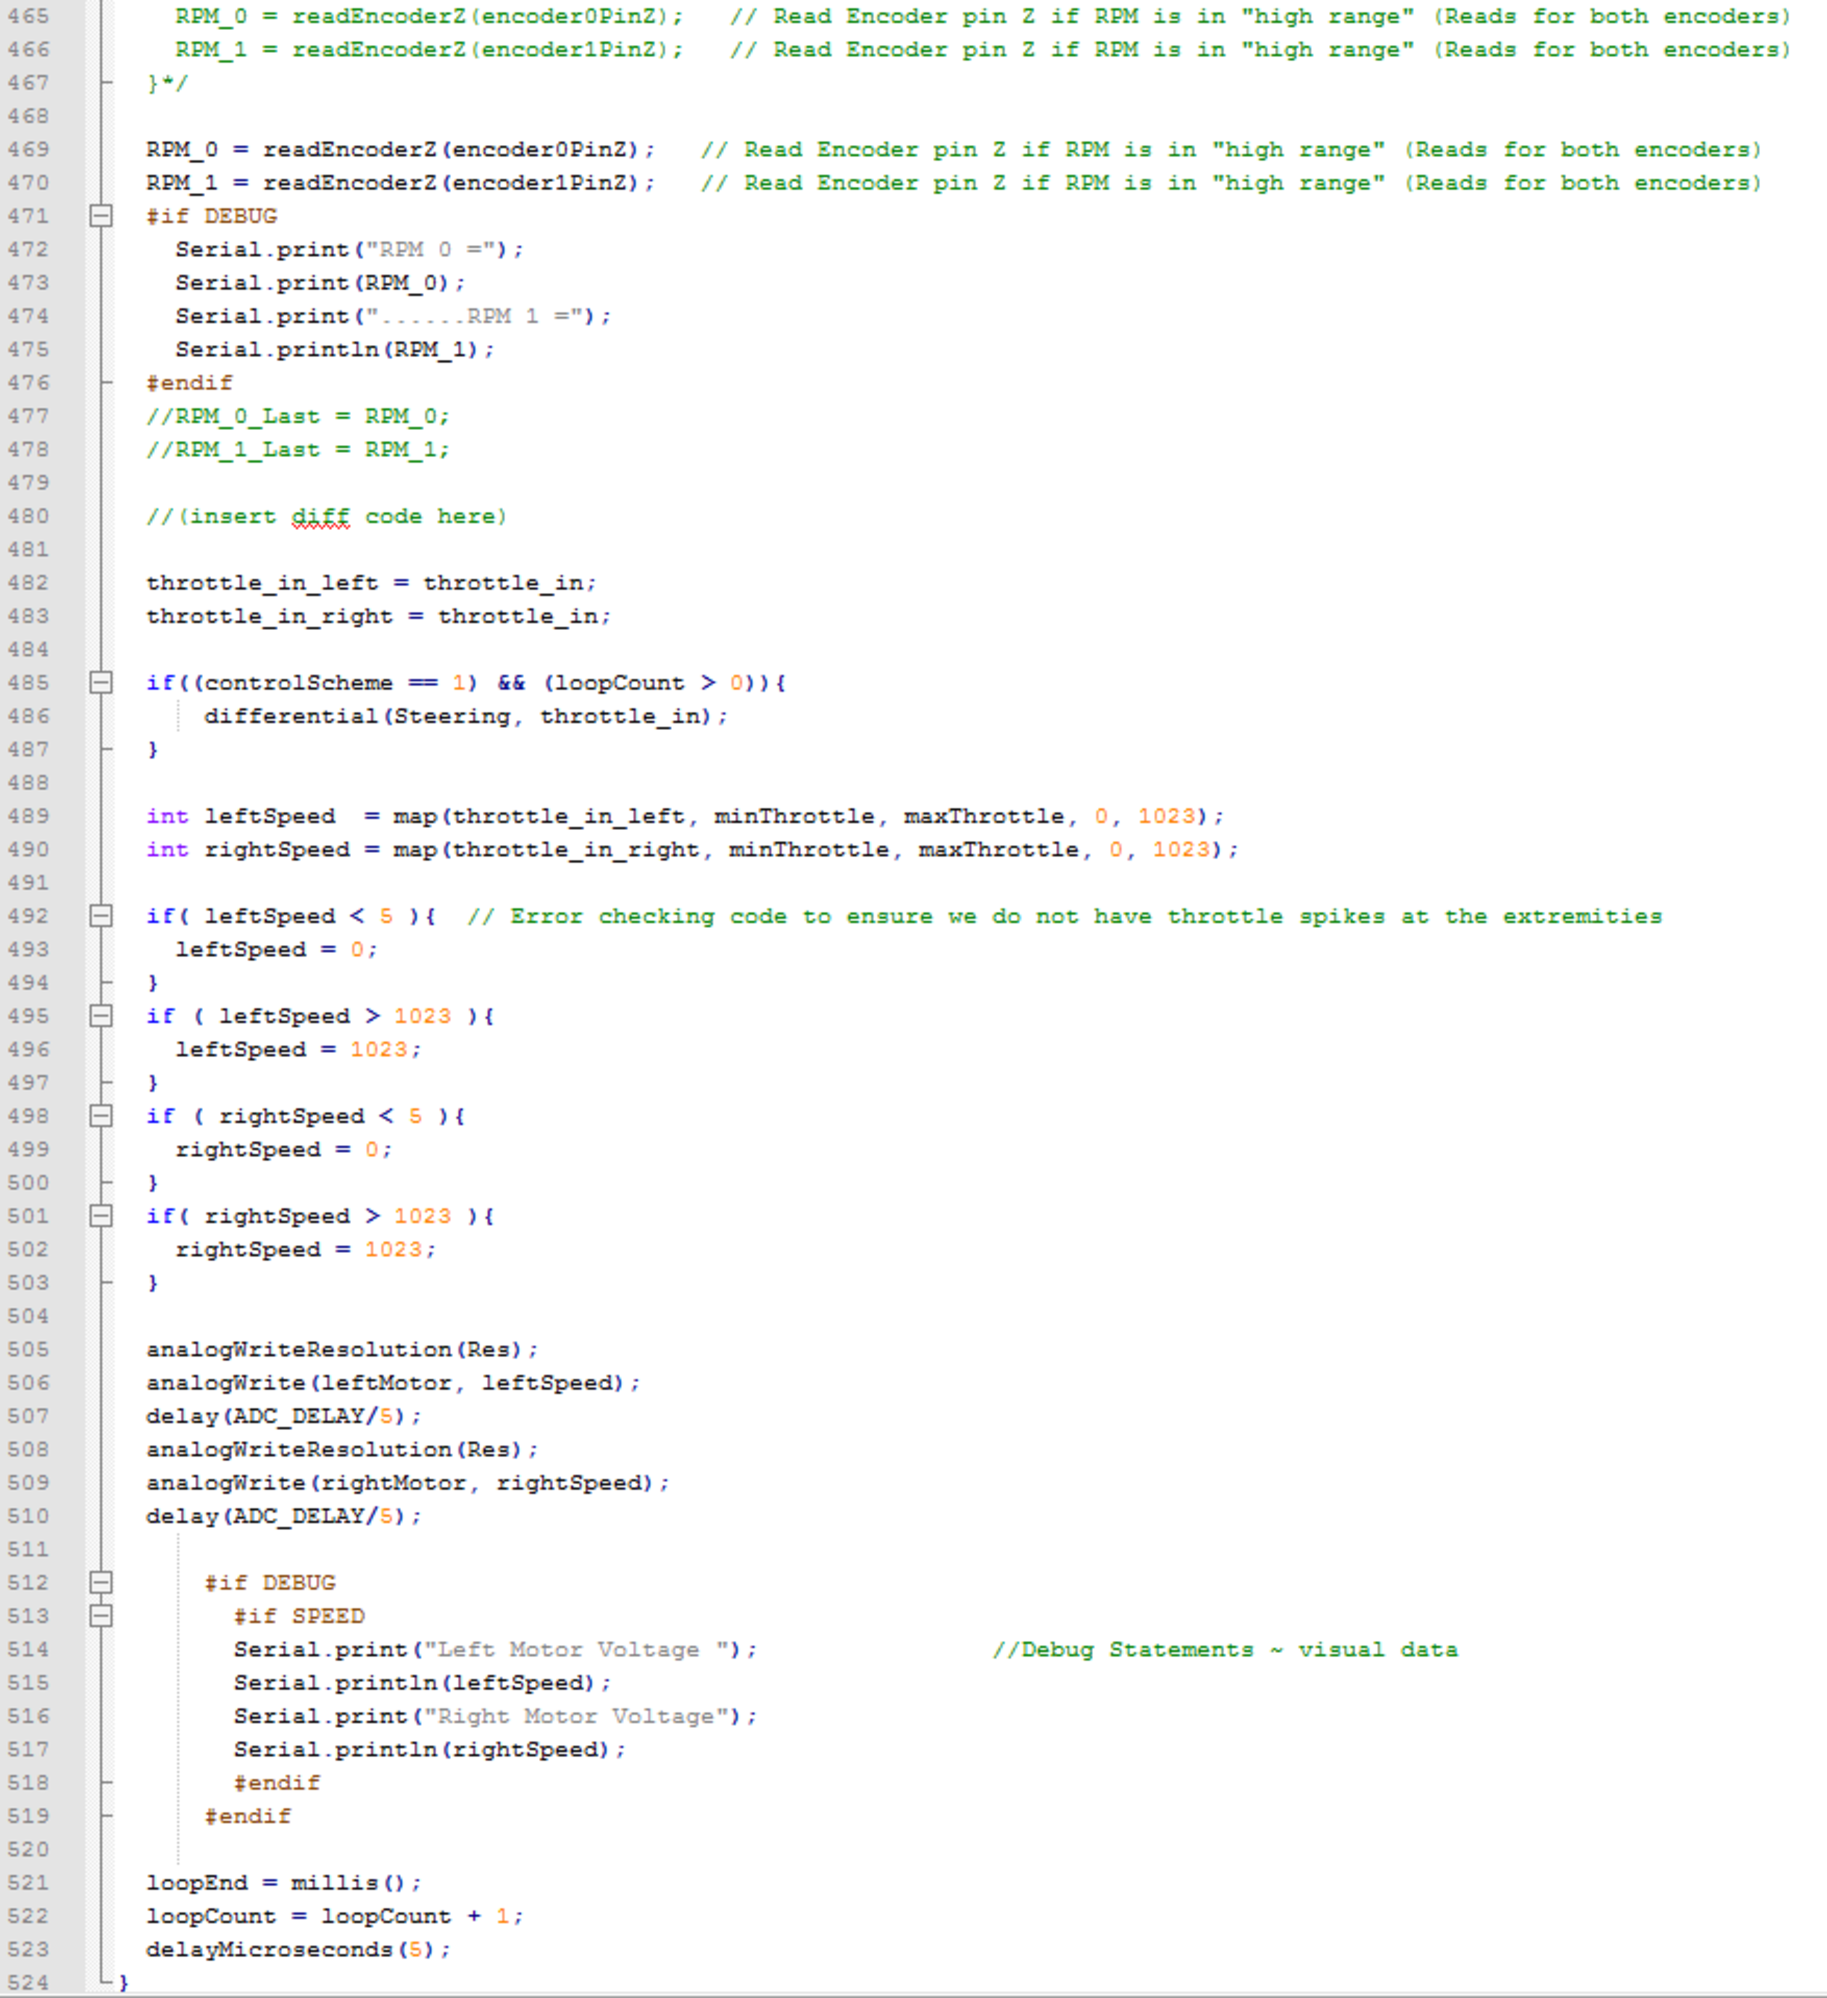
\includegraphics[width=1\textwidth]{code_8.pdf}
\caption*{}
\label{code_8}
\end{figure}
\FloatBarrier


%////////////////////////////////////////////////////////////////////////////////////////////////////////////////////////////////////////////////////////////////////////////////////////////////////////////////////////////////////////
% APPENDIX E
%////////////////////////////////////////////////////////////////////////////////////////////////////////////////////////////////////////////////////////////////////////////////////////////////////////////////////////////////////////
\section{Alternate Ideas}

\subsection{PWM Circuitry}\label{pwm_circuit}

Pulse Width Modulation is a way to map an analog signal to a digital signal. The digital signal is a collection of a square waves. The control of the duty cycle of these waves, will produce an average voltage. The average voltage for the signal is viewed as analog signal for the other devices such as the controllers and  motors.

 In the case of using two different voltages, an auxiliary device needed to control this difference. This case required amplification of the signal from the microprocessor to the motor controllers.  PWM can work greatly to control a solid state relay or to control a transistor. Based on the duty cycle, ON/OFF duration, the transistor is opened and closed to control the voltage seen across the controlled device. The Arduino contain a PWM I/O. Using the analogWrite() function in the microprocessor this functionality is implemented with help of small circuitry. Figure~\ref{pwm_circ} shows the inputs and output of this simple device. The VCC voltage is the maximum voltage needed. The transistor is controlled through one of the Arduino pins. A \SI{1}{\micro\farad} capacitor was added to eliminate noise and chatter in the signal.  

 
 \begin{figure}[!htb]
\centering
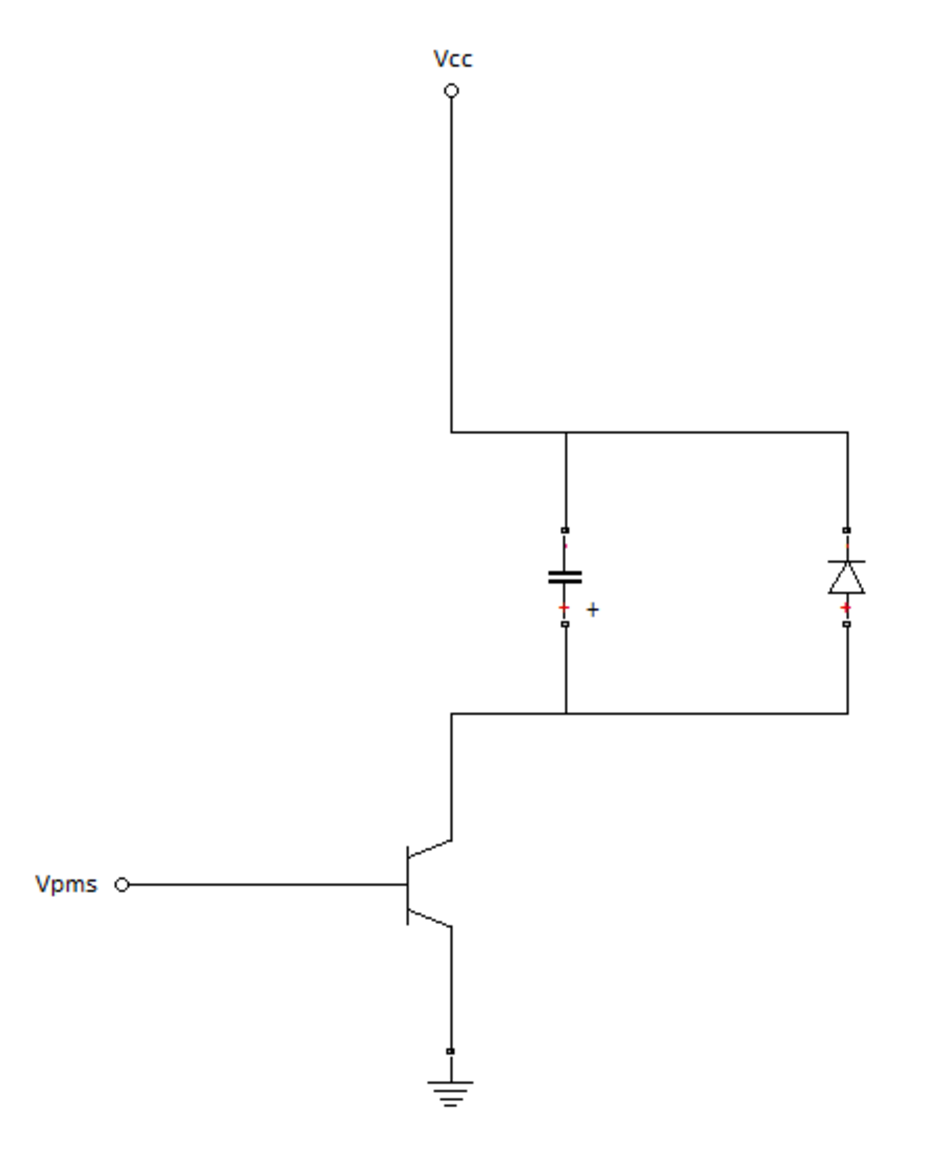
\includegraphics[width=.5\textwidth]{pwm_circuit.pdf}
\caption{PWM Circuit}
\label{pwm_circ}
\end{figure}
\FloatBarrier
 
 

%////////////////////////////////////////////////////////////////////////////////////////////////////////////////////////////////////////////////////////////////////////////////////////////////////////////////////////////////////////
% APPENDIX F
%////////////////////////////////////////////////////////////////////////////////////////////////////////////////////////////////////////////////////////////////////////////////////////////////////////////////////////////////////////
\newpage
\section{Parts \& Data Sheets}

 \begin{figure}[!htb]
\centering
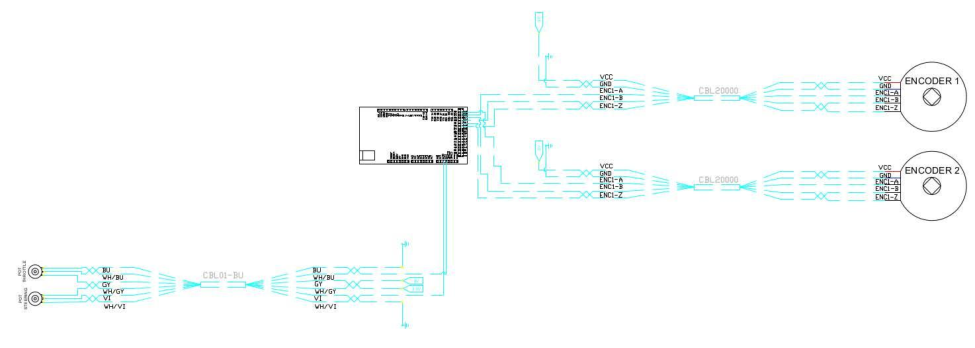
\includegraphics[width=1\textwidth]{sensor_connection.pdf}
\caption{Sensor Connections to Arduino}
\label{sensor_connection}
\end{figure}
\FloatBarrier

 \begin{figure}[!htb]
\centering
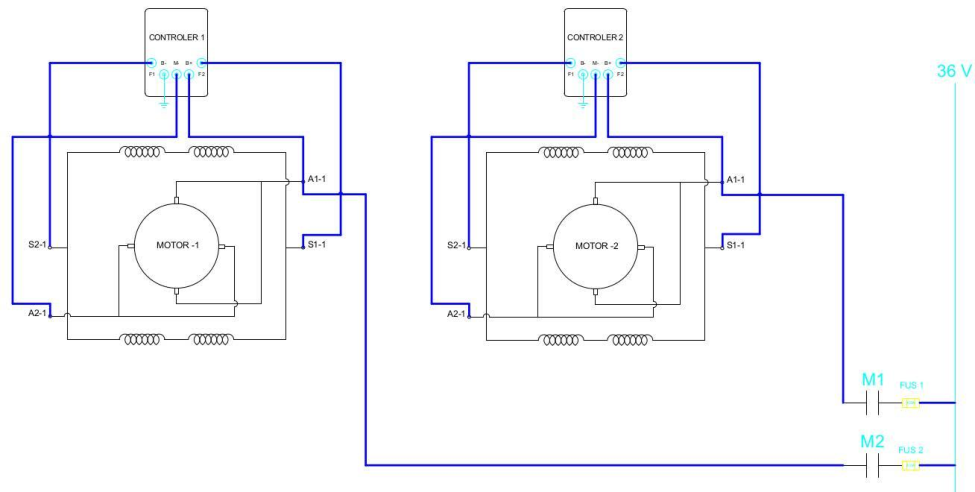
\includegraphics[width=1\textwidth]{battery_connection.pdf}
\caption{Battery Connection to Controllers and Motors}
\label{battery_connection}
\end{figure}
\FloatBarrier

 \begin{figure}[!htb]
\centering
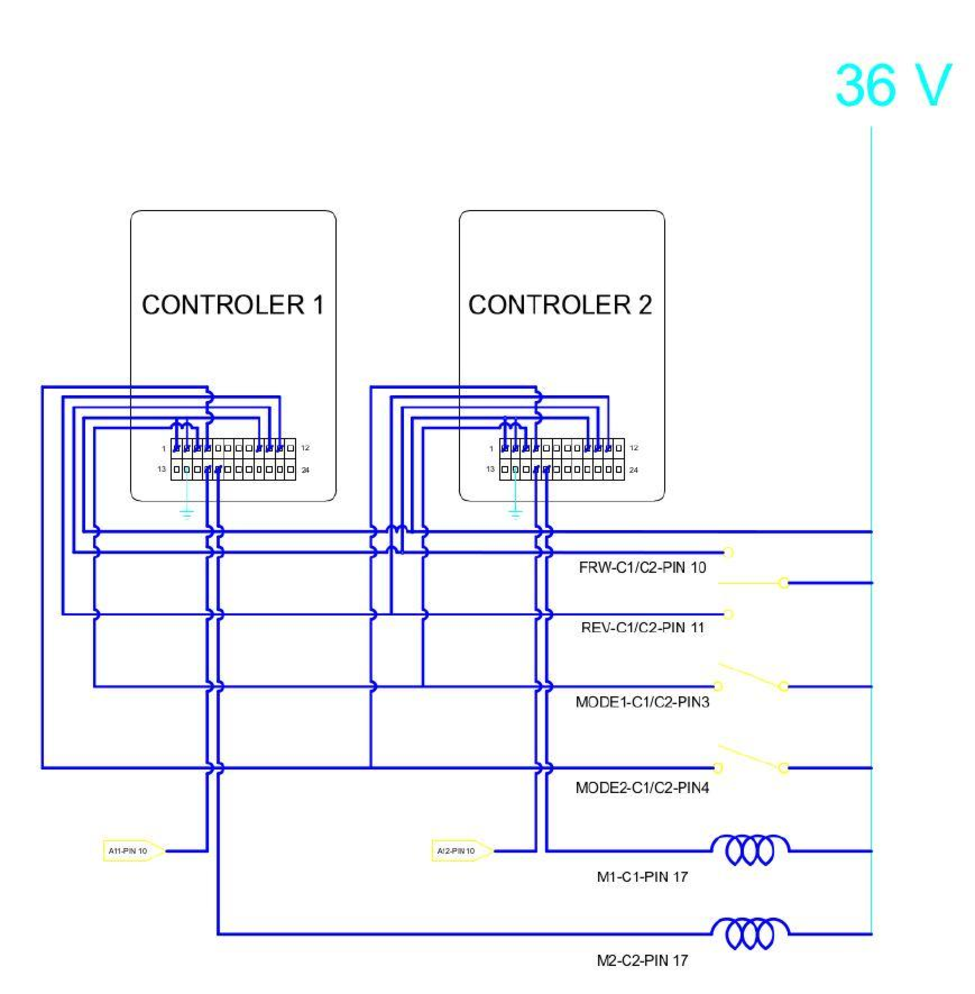
\includegraphics[width=1\textwidth]{control_panel_connections.pdf}
\caption{Control Panel Connections}
\label{control_panel_connections}
\end{figure}
\FloatBarrier

 \begin{figure}[!htb]
\centering
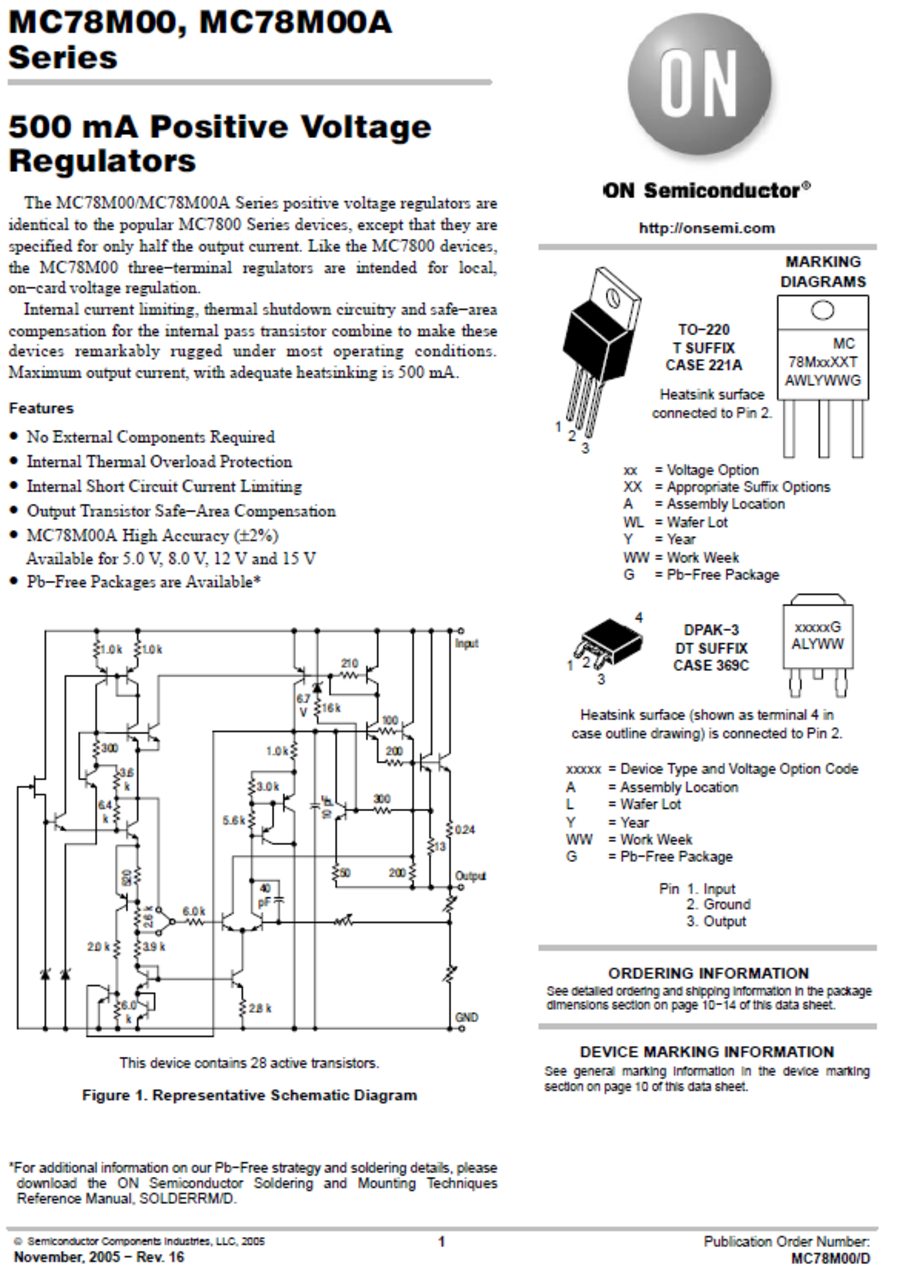
\includegraphics[width=.87\textwidth]{LM7808.pdf}
\caption{LM7808 Voltage Regulator}
\label{LM7808}
\end{figure}
\FloatBarrier


 \begin{figure}[!htb]
\centering
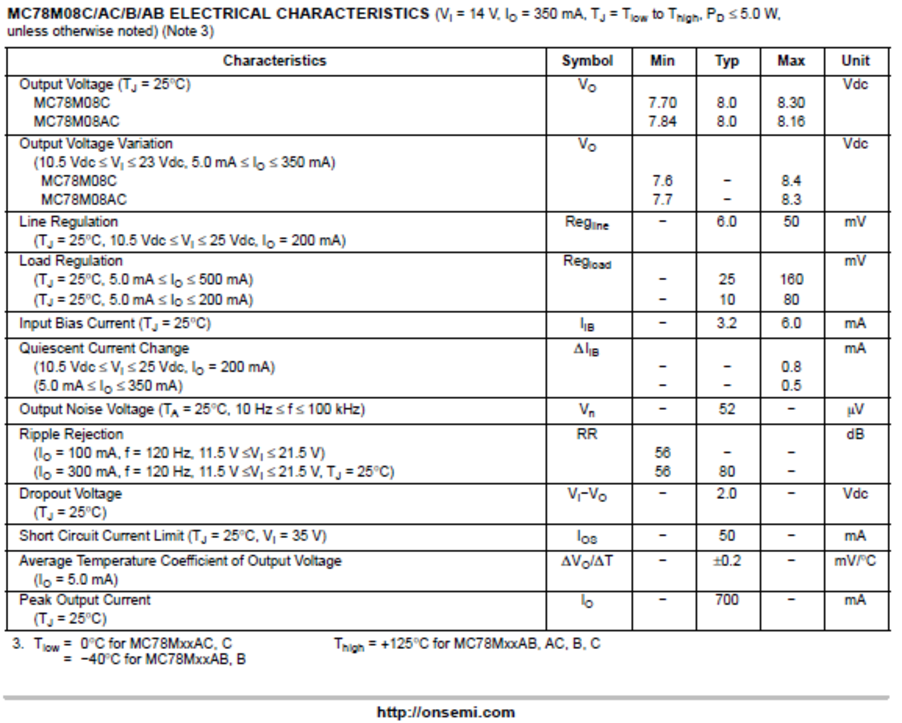
\includegraphics[width=1\textwidth]{MC78.pdf}
\caption{LM7808 Voltage Regulator}
\label{MC78}
\end{figure}
\FloatBarrier


\begin{figure}[!htb]
\centering
\includegraphics[width=.87\textwidth]{LM7660_data.pdf}
\caption{LMC7660 Chip}
\label{LM7660_data}
\end{figure}
\FloatBarrier

 \begin{figure}[!htb]
\centering
\includegraphics[width=.87\textwidth]{LM7660_data_2.pdf}
\caption*{}
\label{LM7660_data_2}
\end{figure}
\FloatBarrier

 \begin{figure}[!htb]
\centering
\includegraphics[width=.87\textwidth]{LM7660_data_3.pdf}
\caption*{}
\label{LM7660_data_3}
\end{figure}
\FloatBarrier

\begin{figure}[!htb]
\centering
\includegraphics[width=.87\textwidth]{LM324_data.pdf}
\caption{LM324 Op Amp}
\label{LM324_data}
\end{figure}
\FloatBarrier

\begin{figure}[!htb]
\centering
\includegraphics[width=1\textwidth]{LM324_data_2.pdf}
\caption*{}
\label{LM324_data_2}
\end{figure}
\FloatBarrier

\begin{figure}[!htb]
\centering
\includegraphics[width=.87\textwidth]{LM324_data_3.pdf}
\caption*{}
\label{LM324_data_3}
\end{figure}
\FloatBarrier

\begin{figure}[!htb]
\centering
\includegraphics[width=.87\textwidth]{LM324_data_4.pdf}
\caption*{}
\label{LM324_data_4}
\end{figure}
\FloatBarrier


\subsection{Curtis Controllers}

\begin{figure}[!htb]
\centering
\includegraphics[width=.87\textwidth]{curtis_1.pdf}
\caption{}
\label{curtis_1}
\end{figure}
\FloatBarrier

\begin{figure}[!htb]
\centering
\includegraphics[width=.87\textwidth]{curtis_2.pdf}
\caption{}
\label{curtis_2}
\end{figure}
\FloatBarrier


\subsection{Batteries}
\begin{figure}[!htb]
\centering
\includegraphics[width=.5\textwidth]{battery_data.pdf}
\caption{Battery Specifications}
\label{battery_data}
\end{figure}
\FloatBarrier


\newpage
\subsection{Solenoids 114-3611-020}
\begin{figure}[!htb]
\centering
\includegraphics[width=.93\textwidth]{solenoid_data.pdf}
\caption{Solenoid Specifications}
\label{solenoid_data}
\end{figure}
\FloatBarrier


\subsection{Upgraded Shocks}
Hydraulic shock with 3'' compression. 730 lbs total load compression. 12'' eye to eye. 10mm (.39'') Hole ID.

\newpage
\subsection{Koyo Optical Encoders}
\begin{figure}[!htb]
\centering
\includegraphics[width=.80\textwidth]{encoders_data.pdf}
\caption{Koyo Optical Encoders Specifications}
\label{koyo_encoders}
\end{figure}
\FloatBarrier


\subsection{VEX Motor Encoders}

The optical shaft encoder is used to measure both relative position of and rotational distance traveled by a shaft. It works by shining light onto the edge of a disk outfitted with evenly spaced slits around the circumference. As the disk spins, light passes through the slits and is blocked by the opaque spaces between the slits. The encoder then detects how many slits have had light shine through, and in which direction the disk is spinning. 

\begin{figure}[!htb]
\centering
\includegraphics[width=.77\textwidth]{vex_encoders_data.pdf}
\caption{VEX Motor Encoders Operation}
\label{vex_encoders}
\end{figure}
\FloatBarrier


Technical Information:
\begin{itemize}
\item Sensor Type: Infrared light sensor and infrared LED
\item Resolution: 90 pulses per revolution
\item Range: No limit, full $360\,^{\circ}$ continuous rotation
\item Size: 2~$\frac{5}{8}$in x 2in
\item Weight: 0.08lb per sensor
\item Shaft Size: $\frac{1}{8}$in square
\item Wiring: Black - ground; Red - (+) power; White - control signal
\end{itemize}


%////////////////////////////////////////////////////////////////////////////////////////////////////////////////////////////////////////////////////////////////////////////////////////////////////////////////////////////////////////
% APPENDIX G
%////////////////////////////////////////////////////////////////////////////////////////////////////////////////////////////////////////////////////////////////////////////////////////////////////////////////////////////////////////

%////////////////////////////////////////////////////////////////////////////////////////////////////////////////////////////////////////////////////////////////////////////////////////////////////////////////////////////////////////
% APPENDIX H
%////////////////////////////////////////////////////////////////////////////////////////////////////////////////////////////////////////////////////////////////////////////////////////////////////////////////////////////////////////

%////////////////////////////////////////////////////////////////////////////////////////////////////////////////////////////////////////////////////////////////////////////////////////////////////////////////////////////////////////
% ACKNOWLEDGEMENTS AND SPECIAL THANKS
%////////////////////////////////////////////////////////////////////////////////////////////////////////////////////////////////////////////////////////////////////////////////////////////////////////////////////////////////////////
\newpage
% use section* for acknowledgement
\ifCLASSOPTIONcompsoc
  % The Computer Society usually uses the plural form
  \section*{Acknowledgments}
\else
  % regular IEEE prefers the singular form
  \section*{Acknowledgment}
\fi

The authors would like to thank...\\

\centering
\begin{tabular}{c c c} 
Carolina Cars and Clubs   & 	Advanced Concepts    & 	Chris Finlayson of\\
					&					   &	 Existential Motorcycles\\
 					&					 &		\\
Mountaintop Golf Cars	 &	EZ-GO (Textron)	   &	Joe and Ellen Reece\\
					&					&		\\
ProMatic Automation	 & 		Dave Erb			 &	Skyland Automotive	\\
					&					&		\\
				& All University of North Carolina Asheville and &\\
				&North Carolina State University Faculty and Staff &\\

\end{tabular} 


% Can use something like this to put references on a page
% by themselves when using endfloat and the captionsoff option.
\ifCLASSOPTIONcaptionsoff
  \newpage
\fi



% trigger a \newpage just before the given reference
% number - used to balance the columns on the last page
% adjust value as needed - may need to be readjusted if
% the document is modified later
%\IEEEtriggeratref{8}
% The "triggered" command can be changed if desired:
%\IEEEtriggercmd{\enlargethispage{-5in}}


%////////////////////////////////////////////////////////////////////////////////////////////////////////////////////////////////////////////////////////////////////////////////////////////////////////////////////////////////////////
% REFERENCES
%////////////////////////////////////////////////////////////////////////////////////////////////////////////////////////////////////////////////////////////////////////////////////////////////////////////////////////////////////////

% can use a bibliography generated by BibTeX as a .bbl file
% BibTeX documentation can be easily obtained at:
% http://www.ctan.org/tex-archive/biblio/bibtex/contrib/doc/
% The IEEEtran BibTeX style support page is at:
% http://www.michaelshell.org/tex/ieeetran/bibtex/
%\bibliographystyle{IEEEtran}
% argument is your BibTeX string definitions and bibliography database(s)
%\bibliography{IEEEabrv,../bib/paper}
%
% <OR> manually copy in the resultant .bbl file
% set second argument of \begin to the number of references
% (used to reserve space for the reference number labels box)
\newpage
\begin{thebibliography}{1}
  
\bibitem{IEEEhowto:kopka}
L.~Brown, \emph{Improving Performance Through Torque Vectoring on an Electric All-Wheel Drive Formula SAE Race Car}. Diss. The University of Western Australia, 2013. Web.
  
\bibitem{IEEEhowto:kopka}
A.~EmranHasan, M. M., M.~Motamed Ektesabi, and A.~Kapoor. \emph{An Investigation into Differential Torque Based Strategies for Electronic Stability Control in an In-Wheel Electric Vehicle}.

\bibitem{IEEEhowto:kopka}
J.~Reza N. \emph{Vehicle Dynamics - Theory and Application}. Springer New York, 2014. 387-495. eBook. \textless http://link.springer.com/book/10.1007/978-1-4614-8544-5\textgreater.

\bibitem{IEEEhowto:kopka}
Z.~Salam. \emph{DC Motor Drive}. \emph{Power Electronics and Drives}. Version 3. (2003): 1-34. Web. 9 Feb. 2014. \textless http://www.docstoc.com/docs/21935976/DC-Motor-Drive\textgreater.

\bibitem{IEEEhowto:kopka}
2014 UNCA/NCSU Senior Design Team. \emph{2wd Electronic Differential}. (2014). GitHub Repository. \textless https://github.com/Ultrashock/EGM484\textgreater.

\bibitem{IEEEhowto:kopka}
J.~Reynold.  \emph{ANSI Standard Roller Chain}.  Web. \\\textless http://www.renoldjeffrey.com/nmsruntime/saveasdialog.asp?lID=1006\&sID=2750\textgreater.

\bibitem{IEEEhowto:kopka}
\emph{Drive with PID Control on an Arduino Mega 2560}. MakerZone. 13 Sept. 2013. \emph{Mathworks, Inc}. 16 Sept. 2013. Web. \textless http://makerzone.mathworks.com/uncategorized/drive-with-pid-control-on-an-arduino-mega-2560/\textgreater.


\end{thebibliography}




%////////////////////////////////////////////////////////////////////////////////////////////////////////////////////////////////////////////////////////////////////////////////////////////////////////////////////////////////////////
% BIOGRAPHY SECTION
%////////////////////////////////////////////////////////////////////////////////////////////////////////////////////////////////////////////////////////////////////////////////////////////////////////////////////////////////////////
% If you have an EPS/PDF photo (graphicx package needed) extra braces are
% needed around the contents of the optional argument to biography to prevent
% the LaTeX parser from getting confused when it sees the complicated
% \includegraphics command within an optional argument. (You could create
% your own custom macro containing the \includegraphics command to make things
% simpler here.)
%\begin{IEEEbiography}[{\includegraphics[width=1in,height=1.25in,clip,keepaspectratio]{mshell}}]{Michael Shell}
% or if you just want to reserve a space for a photo:

%\begin{IEEEbiography}{Michael Shell}
%Biography text here.
%\end{IEEEbiography}
%
%% if you will not have a photo at all:
%\begin{IEEEbiographynophoto}{John Doe}
%Biography text here.
%\end{IEEEbiographynophoto}
%
%% insert where needed to balance the two columns on the last page with
%% biographies
%%\newpage
%
%\begin{IEEEbiographynophoto}{Jane Doe}
%Biography text here.
%\end{IEEEbiographynophoto}

% You can push biographies down or up by placing
% a \vfill before or after them. The appropriate
% use of \vfill depends on what kind of text is
% on the last page and whether or not the columns
% are being equalized.

%\vfill

% Can be used to pull up biographies so that the bottom of the last one
% is flush with the other column.
%\enlargethispage{-5in}



% that's all folks
\end{document}


